% Saberes básicos (LOMLOE) asociados a esta unidad
%----------------------------------------------------------------------------------------
% A. Las destrezas científicas básicas
%   - Metodologías de la investigación científica: se introduce el método científico
%     (observación, hipótesis, experimentación, análisis de resultados y conclusiones) como
%     forma de trabajo propia de la física y la química, con ejemplos y un ejercicio de
%     identificación de sus fases en una investigación sencilla.
%   - El lenguaje científico: unidades del Sistema Internacional y sus símbolos: toda la unidad
%     gira en torno al SI (magnitud, unidad, medida), sus múltiplos y submúltiplos, y las reglas
%     de escritura correcta de los símbolos.
%   - Herramientas matemáticas básicas en diferentes escenarios científicos: uso de factores de
%     conversión, reglas de tres y ecuaciones sencillas (d = m/V) para resolver problemas
%     cuantitativos de conversión de unidades y de cálculo de magnitudes.
%   - Diversos entornos y recursos de aprendizaje científico como el laboratorio: manejo de
%     balanzas, probetas, buretas y pipetas; lectura correcta de instrumentos (menisco,
%     sensibilidad, precisión y exactitud de una medida).
%   - Normas de uso de cada espacio, asegurando y protegiendo así la salud propia y comunitaria
%     (identificación del material de laboratorio, normas generales de seguridad y pictogramas
%     de peligrosidad de los productos químicos, SGA/GHS) y el respeto hacia el medio ambiente.
%
% B. La materia
%   - Experimentos relacionados con los sistemas materiales: conocimiento y descripción de sus
%     propiedades (generales/características, cuantitativas/cualitativas, extensivas/intensivas),
%     su clasificación en cuerpos y sistemas materiales, y el uso de la densidad relativa para
%     predecir si un cuerpo flota o se hunde en un líquido.
%
% (Esta unidad no desarrolla contenidos de los bloques C -la energía-, D -la interacción- ni
% E -el cambio-, que se trabajan en unidades posteriores del curso.)
%----------------------------------------------------------------------------------------

\spacing{1.3}
\raggedbottom % pages with large figures end where the text ends (no stretched gaps between boxes)

%\section{Science and the scientific method}
%
%\begin{definition}[Science]
%    A human activity that explains how nature works, in an organised way that can be tested.
%\end{definition}
%
%Scientists answer their questions by following a set of steps called the \negsubro{scientific method}.
%
%\begin{figure}[H]
%    \centering
%    \includegraphics[width=\textwidth]{Unit_1/scientific_method}
%    \caption{The five steps of the scientific method.}
%    \label{fig:u1_scientific_method}
%\end{figure}
%
%\begin{example}
%
%    \begin{enumerate}[label=\numberballmDarkTeal]
%        \item \textbf{Observation}: the plants in a dark corner of the classroom look pale.
%        \item \textbf{Hypothesis}: ``plants need light to stay green''.
%        \item \textbf{Experiment}: identical plants, same water and soil; some in the light, some in the dark.
%        \item \textbf{Analysis}: after two weeks we measure their colour and height.
%        \item \textbf{Conclusion}: plants in the light are green, the others are pale. The hypothesis is accepted.
%    \end{enumerate}
%\end{example}
%
%\begin{impt}
%    In a good experiment we change \textbf{only one variable} (the light) and keep all the others the same (water, soil, temperature\ldots). That way we know exactly what caused the result.
%\end{impt}
%
%\begin{didyouknow}
%    Alexander Fleming discovered penicillin in 1928 thanks to an \emph{observation}: a mould had killed the bacteria in one of his dishes. Asking ``why?'' was the first step of a discovery that has saved millions of lives.
%\end{didyouknow}
%
%\begin{exercise}
%    A group of students wants to find out whether sugar dissolves faster in hot water or in cold water. Identify, in this investigation, the observation, the hypothesis, the experiment and a possible conclusion.
%    \begin{solu}
%        \textbf{Observation}: sometimes sugar seems to dissolve faster than other times. \\
%        \textbf{Hypothesis}: sugar dissolves faster in hot water than in cold water. \\
%        \textbf{Experiment}: dissolve the same amount of sugar in two identical glasses, one with hot water and one with cold water, stirring in the same way, and measure the time it takes to dissolve completely. \\
%        \textbf{Conclusion}: if the sugar dissolves in less time in the hot water, the hypothesis is confirmed.
%    \end{solu}
%\end{exercise}
%
%\begin{exercise}
%    Say which step of the scientific method (observation, hypothesis, experimentation, analysis of results or conclusions) each sentence describes:
%    \begin{enumerate}[label=\letraminuscula]
%        \item ``Plants watered with fertiliser grow taller than plants watered only with water.''
%        \item ``I think that music helps plants grow faster.''
%        \item ``I water ten identical plants with music and ten without, keeping everything else the same, and measure their height every week.''
%        \item ``I notice that the bread in the kitchen goes mouldy faster in summer than in winter.''
%    \end{enumerate}
%    \begin{solu}
%        \begin{enumerate}[label=\alph*)]
%            \item Conclusion (a statement accepted after comparing results).
%            \item Hypothesis (a testable, proposed explanation).
%            \item Experimentation (the procedure designed to test the hypothesis).
%            \item Observation (a fact that raises a question).
%        \end{enumerate}
%    \end{solu}
%\end{exercise}
%
%\begin{exercise}
%    Explain, in your own words, why in a well-designed experiment scientists change only one variable at a time. Give an example of what could go wrong if two variables were changed at once.
%    \begin{solu}
%        If more than one variable changes at the same time, we cannot know which one is responsible for the result. \\
%        For example, if we water some plants with fertiliser \emph{and} give them more light, and they grow taller, we would not know whether it was the fertiliser, the light, or both.
%    \end{solu}
%\end{exercise}

%----------------------------------------------------------------------------------------

\section{Matter and its properties}

\begin{definition}[Matter]
    Everything that has \textbf{mass} and occupies \textbf{space}.
\end{definition}

\begin{figure}[H]
    \centering
    % [FIGURA ORIGINAL] \includegraphics[width=\textwidth]{Unit_1/matter_definition}
    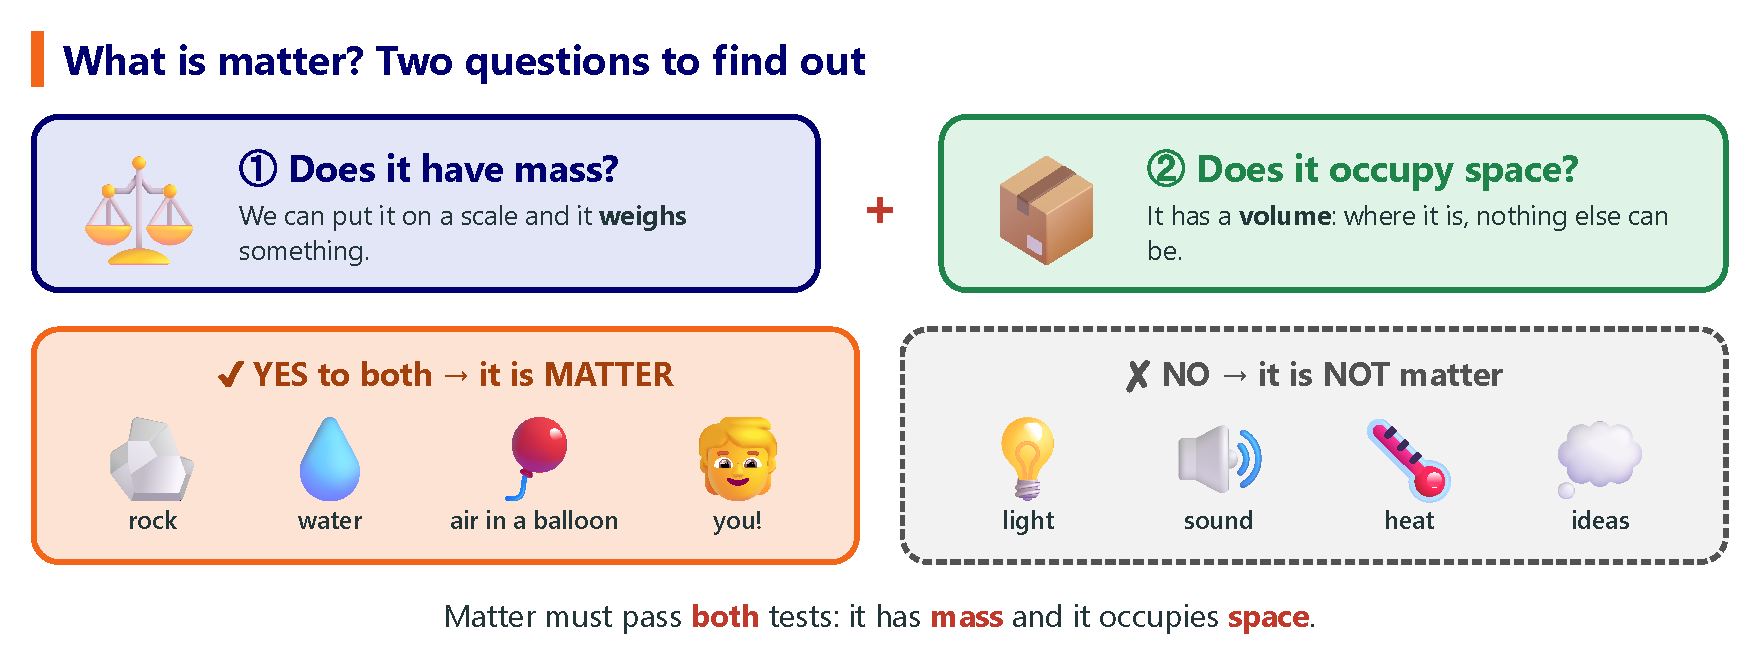
\includegraphics[width=\textwidth]{FigurasSVG/Unit_1_Matter_Measurement/pdf/matter_definition.pdf}
    \caption{To be matter, something must have mass \textbf{and} occupy space. Light, sound, heat or ideas are not matter.}
    \label{fig:u1_matter_definition}
\end{figure}

The bench you sit on, the water you drink and your own body are all matter. Matter is divided into two big groups: \negsubro{bodies} and \negsubro{material systems}.

\begin{definition}[Body]
    A portion of matter that has its \textbf{own shape} and \textbf{defined boundaries}: we can see where it begins and where it ends. For example, a ball, a pencil, a chair or the Moon.
\end{definition}

\begin{definition}[Material system]
    A portion of matter that has \textbf{no shape of its own} and \textbf{no defined boundaries}: it takes the shape of the container that holds it. For example, milk, air, juice or petrol.
\end{definition}

\begin{figure}[H]
    \centering
    % [FIGURA ORIGINAL] \includegraphics[width=\textwidth]{Unit_1/matter_scheme}
    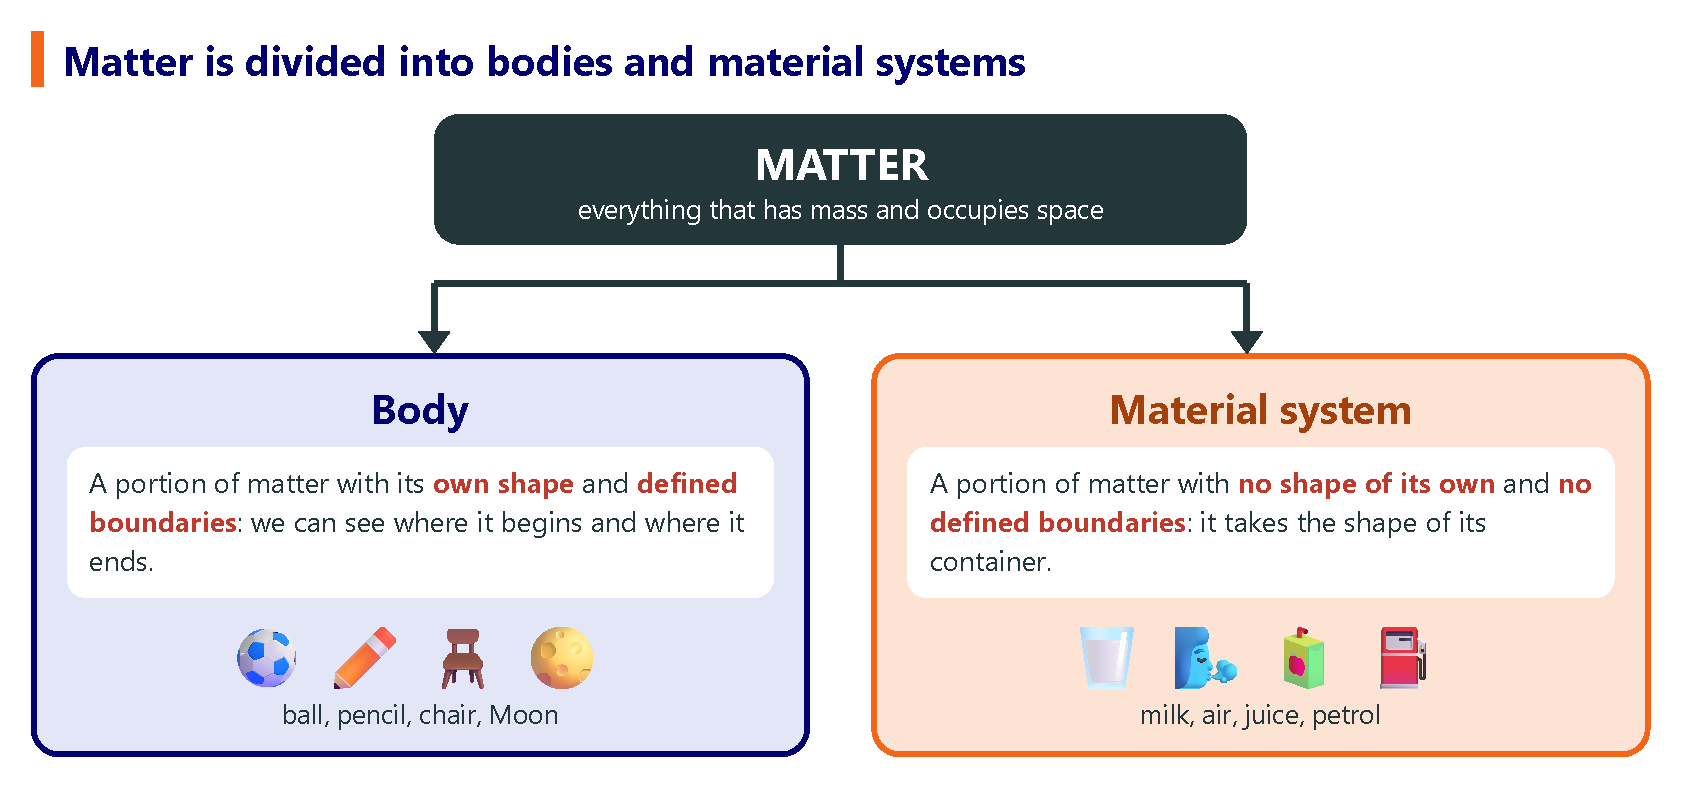
\includegraphics[width=\textwidth]{FigurasSVG/Unit_1_Matter_Measurement/pdf/matter_scheme.pdf}
    \caption{Scheme: matter is divided into bodies and material systems.}
    \label{fig:u1_matter_scheme}
\end{figure}

\begin{figure}[H]
    \centering
    % [FIGURA ORIGINAL] \includegraphics[width=\textwidth]{Unit_1/matter_bodies}
    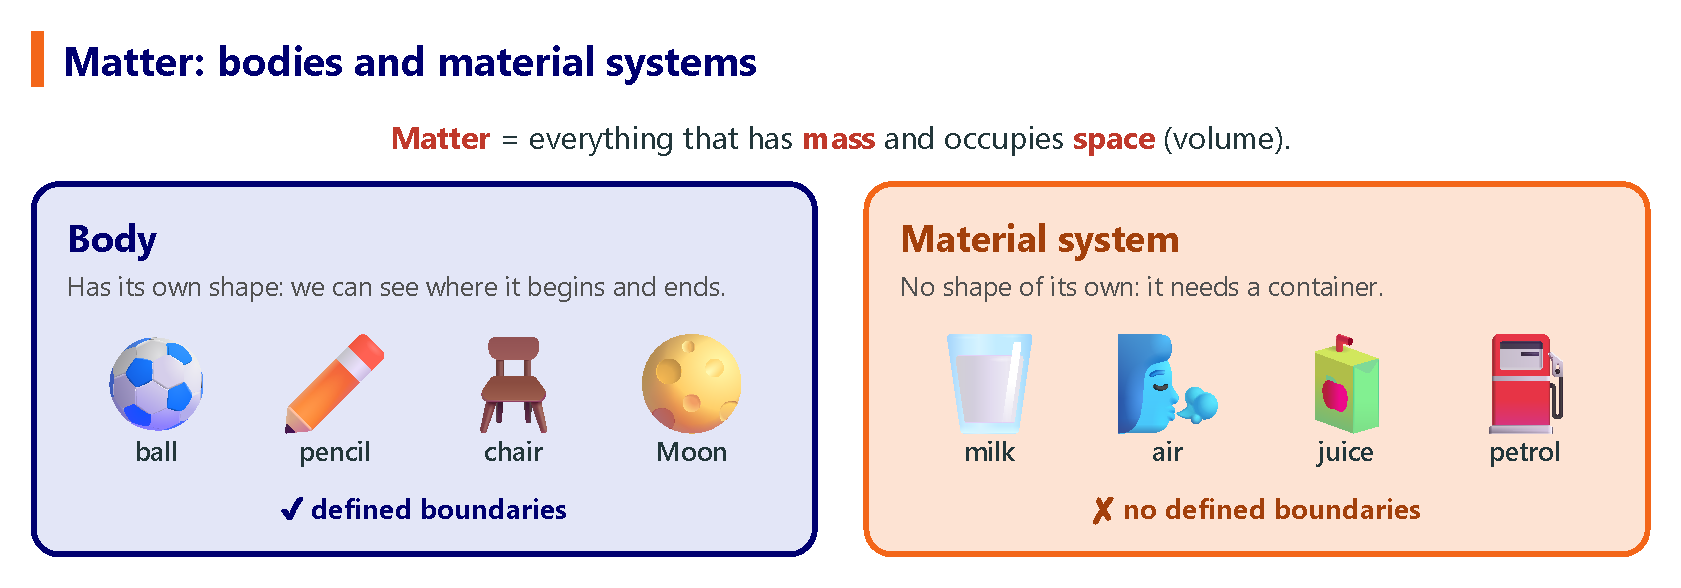
\includegraphics[width=\textwidth]{FigurasSVG/Unit_1_Matter_Measurement/pdf/matter_bodies.pdf}
    \caption{Bodies have their own shape; material systems need a container.}
    \label{fig:u1_matter_bodies}
\end{figure}

\begin{exercise}
    Say whether each of these things is \textbf{matter} or \textbf{not matter}. Remember: to be matter it must have mass \textbf{and} occupy space.
    \begin{enumerate}[label=\letraminuscula]
        \item The air in a room.
        \item Sunlight.
        \item A stone.
        \item The sound of a bell.
        \item A cloud.
        \item The heat from a radiator.
        \item A dream.
        \item The smoke from a fire.
        \item A rainbow.
        \item A drop of oil.
    \end{enumerate}
    \begin{solu}
        \begin{enumerate}[label=\alph*)]
            \item Matter (air has mass and fills the room).
            \item Not matter (light has no mass).
            \item Matter.
            \item Not matter (sound is a vibration that travels through matter, but it is not matter).
            \item Matter (it is made of tiny drops of water).
            \item Not matter (heat is energy).
            \item Not matter (an idea has no mass and does not occupy space).
            \item Matter (it is made of gases and tiny solid particles).
            \item Not matter (it is light).
            \item Matter.
        \end{enumerate}
    \end{solu}
\end{exercise}

\begin{exercise}
    Say whether each of these portions of matter is a \textbf{body} or a \textbf{material system}:
    \begin{enumerate}[label=\letraminuscula]
        \item A coin.
        \item Sea water.
        \item A key.
        \item The oxygen inside a balloon.
        \item Honey.
        \item A pencil.
        \item Olive oil.
        \item A glass marble.
        \item Steam.
        \item A tennis ball.
    \end{enumerate}
    \begin{solu}
        \begin{enumerate}[label=\alph*)]
            \item Body (own shape and defined boundaries).
            \item Material system (it takes the shape of the sea bed or of the container).
            \item Body.
            \item Material system (the gas takes the shape of the balloon).
            \item Material system (it takes the shape of the jar).
            \item Body.
            \item Material system.
            \item Body.
            \item Material system.
            \item Body.
        \end{enumerate}
    \end{solu}
\end{exercise}

\subsection{Physics and chemistry}

Physics and chemistry are the two sciences that study matter and its changes:

\begin{itemize}
    \item \textbf{Physics} studies \negsubro{physical changes}: the substance stays \textbf{the same}.
    \item \textbf{Chemistry} studies \negsubro{chemical changes}: \textbf{new substances} appear.
\end{itemize}

\begin{figure}[H]
    \centering
    % [FIGURA ORIGINAL] \includegraphics[width=\textwidth]{Unit_1/physical_chemical}
    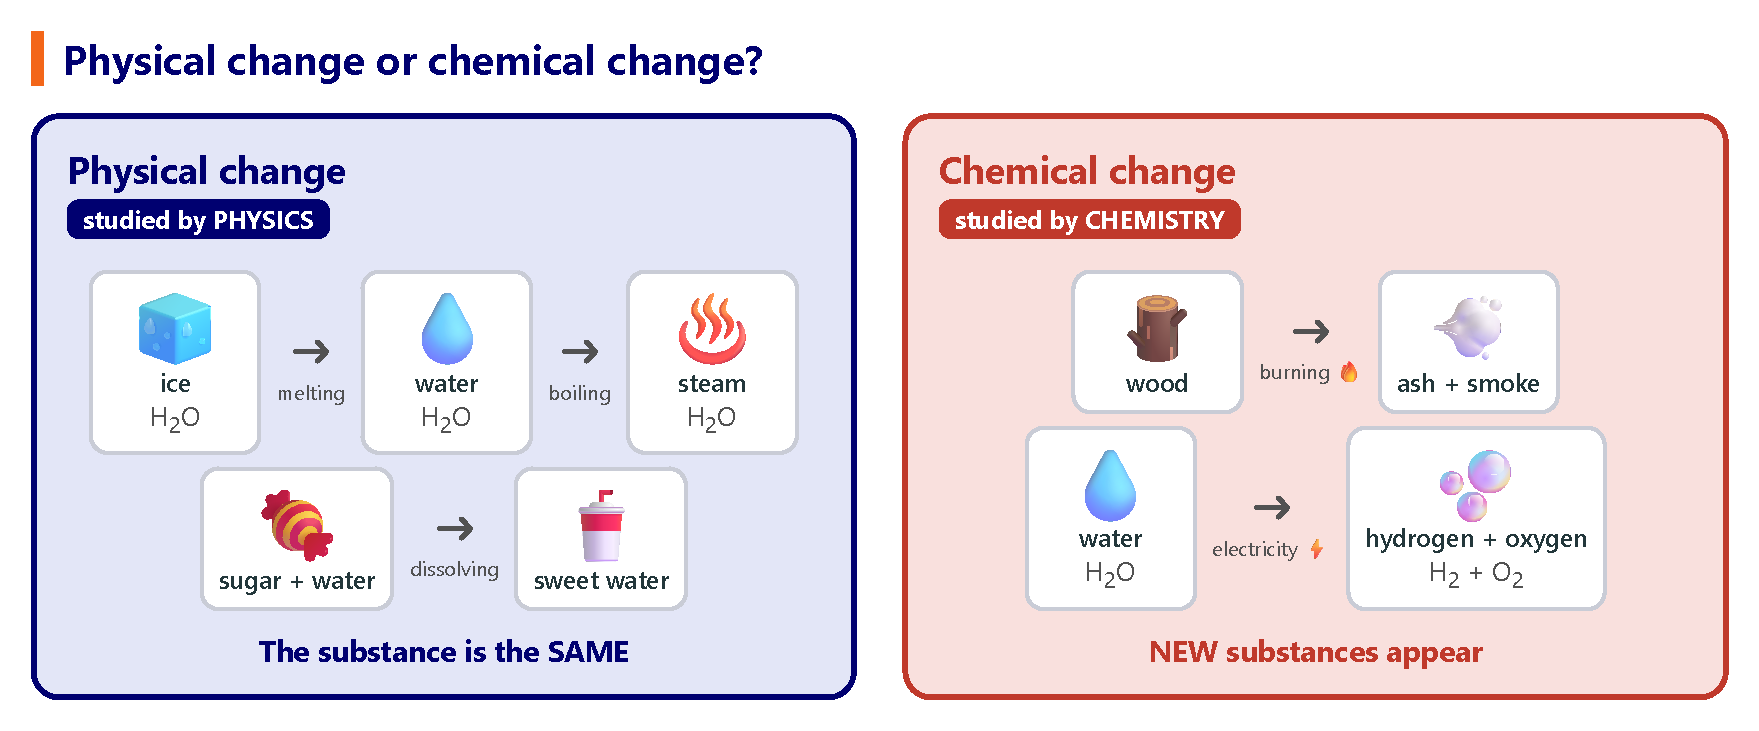
\includegraphics[width=\textwidth]{FigurasSVG/Unit_1_Matter_Measurement/pdf/physical_chemical.pdf}
    \caption{In a physical change the substance is the same; in a chemical change new substances are formed.}
    \label{fig:u1_physical_chemical}
\end{figure}

\begin{impt}
    \textbf{Quick test}: ask yourself ``\emph{Is it still the same substance at the end?}'' If the answer is \textbf{yes} \(\to\) physical change. If \textbf{no} \(\to\) chemical change.
\end{impt}

\begin{exercise}
    Classify these examples as \textbf{physical} or \textbf{chemical} changes:
    \begin{enumerate}[label=\letraminuscula]
        \item Dissolving sugar in water.
        \item Burning wood.
        \item Grinding food.
        \item Moulding a piece of clay.
        \item Melting ice cream.
        \item Frying a steak.
    \end{enumerate}
    \begin{solu}
        \begin{enumerate}[label=\alph*)]
            \item Physical (the sugar is still sugar, only mixed with water).
            \item Chemical (new substances such as ash and smoke appear).
            \item Physical (the food changes shape, not composition).
            \item Physical (only the shape changes).
            \item Physical (change of state, from solid to liquid).
            \item Chemical (the food's composition changes when cooked).
        \end{enumerate}
    \end{solu}
\end{exercise}

\begin{exercise}
    Classify these terms as \textbf{bodies} or \textbf{material systems}:

    Book, phone, aluminium, juice, air, atmosphere, bottle of water, bird, Moon.
    \begin{solu}
        \textbf{Bodies}: book, phone, bottle of water, bird, Moon (they have defined boundaries). \\
        \textbf{Material systems}: aluminium, juice, air, atmosphere (they have no defined boundaries of their own).
    \end{solu}
\end{exercise}

\begin{exercise}
    Say whether physics or chemistry would study each situation, and explain why:
    \begin{enumerate}[label=\letraminuscula]
        \item A metal bar getting longer when it is heated.
        \item A nail rusting after being left outside in the rain.
        \item A ball rolling down a ramp.
        \item Milk turning sour and forming yoghurt.
    \end{enumerate}
    \begin{solu}
        \begin{enumerate}[label=\alph*)]
            \item Physics: the bar is still the same metal, only its size changes.
            \item Chemistry: rust (iron oxide) is a new substance, different from iron.
            \item Physics: the ball's composition does not change, only its position and speed.
            \item Chemistry: yoghurt is a different substance from milk.
        \end{enumerate}
    \end{solu}
\end{exercise}

\subsection{Properties of matter}

\begin{definition}[Property of matter]
    Any aspect of matter that we can observe or measure.
\end{definition}

We classify properties by answering three questions:

\begin{figure}[H]
    \centering
    % [FIGURA ORIGINAL] \includegraphics[width=\textwidth]{Unit_1/properties_map}
    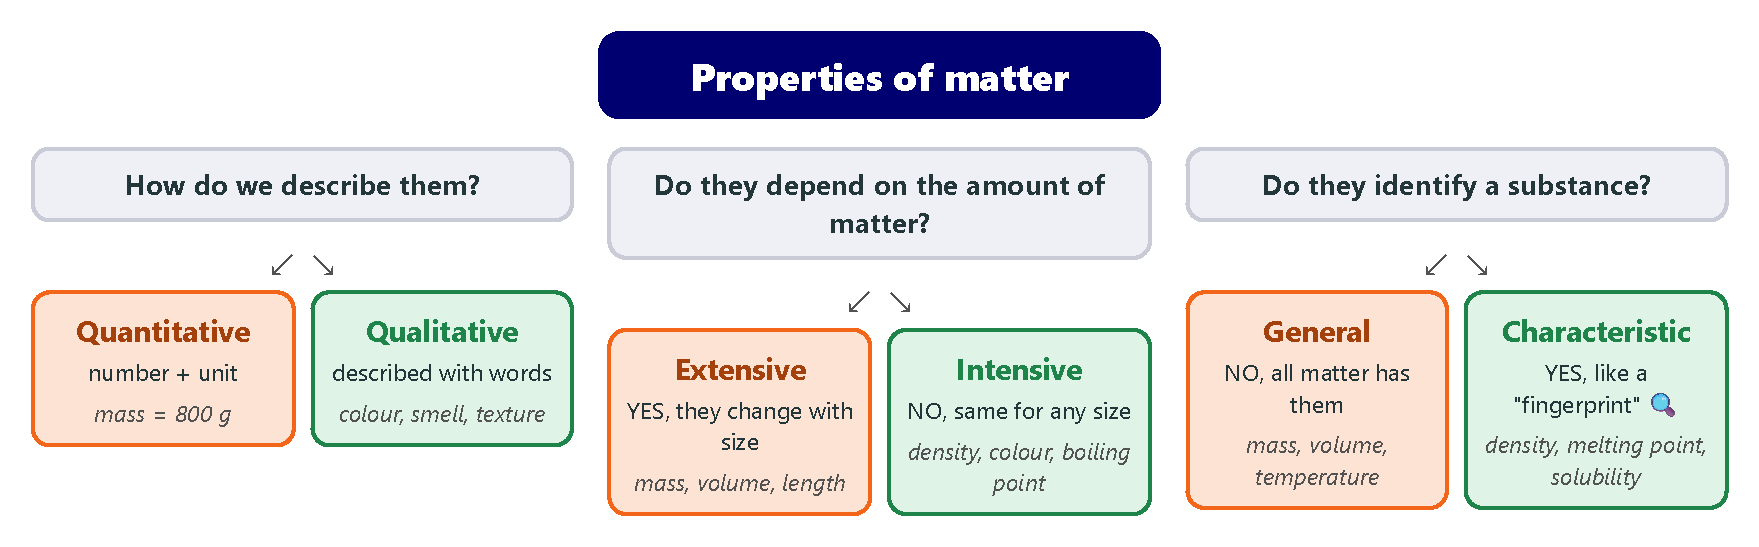
\includegraphics[width=\textwidth]{FigurasSVG/Unit_1_Matter_Measurement/pdf/properties_map.pdf}
    \caption{Three ways of classifying the properties of matter.}
    \label{fig:u1_properties_map}
\end{figure}

These three questions are \textbf{independent}, so we must answer \textbf{all three} for every property. In other words, the \textbf{same property} is, at the same time, of one type in each classification:

\begin{table}[H]
    \centering
    \small
    \renewcommand{\arraystretch}{1.35}
    \begin{tabular}{p{2.4cm}p{3.2cm}p{3.4cm}p{3.4cm}}
        \toprule
        \textbf{Property} & \textbf{How do we describe it?} & \textbf{Does it depend on the amount?} & \textbf{Does it identify a substance?} \\
        \midrule
        Mass & quantitative & extensive & general \\
        Volume & quantitative & extensive & general \\
        Temperature & quantitative & intensive & general \\
        Density & quantitative & intensive & characteristic \\
        Boiling point & quantitative & intensive & characteristic \\
        Colour & qualitative & intensive & characteristic \\
        \bottomrule
    \end{tabular}
    \caption{Each property is classified in the three ways at the same time.}
    \label{tab:u1_three_classifications}
\end{table}

\begin{impt}
    A property is never ``only'' quantitative or ``only'' intensive. For example, \textbf{density} is \textbf{quantitative} (\qty{1.00}{\g\per\mL}), \textbf{intensive} (a drop of water and a swimming pool have the same density) and \textbf{characteristic} (it helps us to identify water).
\end{impt}

\negsubro{Characteristic properties} are the ``fingerprint'' of a substance: they help us to identify it.

\begin{table}[H]
    \centering
    \small
    \renewcommand{\arraystretch}{1.35}
    \begin{tabular}{p{2.2cm}p{3.8cm}p{3.0cm}p{3.2cm}}
        \toprule
        \textbf{Property} & \textbf{What it tells us} & \textbf{Type} & \textbf{Example} \\
        \midrule
        Density & mass in each unit of volume, \(d = m/V\) & quantitative, intensive, characteristic & water: \qty{1.00}{\g\per\mL} \\
        Melting point & temperature at which a solid melts & quantitative, intensive, characteristic & ice: \qty{0}{\celsius} \\
        Boiling point & temperature at which a liquid boils & quantitative, intensive, characteristic & water: \qty{100}{\celsius} \\
        Solubility & how much dissolves in \qty{100}{\g} of water & quantitative, intensive, characteristic & sugar: yes; oil: no \\
        Conductivity & whether it lets heat and electricity pass & quantitative, intensive, characteristic & metals: yes; wood: no \\
        Hardness & resistance to being scratched (scale 1--10) & quantitative, intensive, characteristic & talc: 1; diamond: 10 \\
        \bottomrule
    \end{tabular}
    \caption{Characteristic properties of matter.}
    \label{tab:u1_characteristic}
\end{table}

\begin{exercise}
    Classify each property in the \textbf{three} ways: \textbf{qualitative} or \textbf{quantitative}, \textbf{extensive} or \textbf{intensive}, and \textbf{general} or \textbf{characteristic}.
    \begin{enumerate}[label=\letraminuscula]
        \item Length.
        \item Smell.
        \item Melting point.
        \item Weight.
        \item Hardness.
        \item Shine (lustre) of a metal.
        \item Electrical conductivity.
        \item Taste.
    \end{enumerate}
    \begin{solu}
        \begin{enumerate}[label=\alph*)]
            \item Quantitative, extensive, general.
            \item Qualitative, intensive, characteristic.
            \item Quantitative, intensive, characteristic.
            \item Quantitative, extensive, general.
            \item Quantitative, intensive, characteristic.
            \item Qualitative, intensive, characteristic.
            \item Quantitative, intensive, characteristic.
            \item Qualitative, intensive, characteristic.
        \end{enumerate}
    \end{solu}
\end{exercise}

\begin{exercise}
    Lucía describes her gold ring. Say which property each sentence describes and \textbf{all} its types (each property has one type in each of the three classifications):
    \begin{enumerate}[label=\letraminuscula]
        \item ``The ring has a mass of \qty{6}{\g}.''
        \item ``Gold is yellow and shiny.''
        \item ``Gold melts at \qty{1064}{\celsius}.''
        \item ``The ring occupies \qty{0.31}{\mL}.''
        \item ``The density of gold is \qty{19.3}{\g\per\mL}.''
        \item ``The ring is at \qty{36}{\celsius} because I am wearing it.''
    \end{enumerate}
    \begin{solu}
        \begin{enumerate}[label=\alph*)]
            \item Mass: quantitative, extensive, general.
            \item Colour and shine: qualitative, intensive, characteristic.
            \item Melting point: quantitative, intensive, characteristic.
            \item Volume: quantitative, extensive, general.
            \item Density: quantitative, intensive, characteristic.
            \item Temperature: quantitative, intensive, general.
        \end{enumerate}
    \end{solu}
\end{exercise}



%----------------------------------------------------------------------------------------

\section{Measurement}

% Cancelled unit (in red) for the conversion factors of this section
\providecommand{\cancelunit}[1]{\cancelred{\unit{#1}}}

\begin{definition}[Quantity]
    Any property of matter that can be measured.
\end{definition}

\begin{definition}[Unit]
    A known amount of a quantity, used as a reference to measure that quantity.
\end{definition}

%\begin{definition}[Measure]
%    To measure a quantity, we compare it with a unit to find how many times that unit is contained in it. The result is a \textbf{number} (amount) followed by a \textbf{unit}.
%\end{definition}

To measure a quantity, we compare it with a unit to find how many times that unit is contained in it. The result is a \textbf{number} (amount) followed by a \textbf{unit}.

\begin{example}
    Length of a battery = \qty{5.0}{\cm}. Here, \(\num{5.0}\) is the amount and \(\unit{\cm}\) is the unit.
\end{example}

\subsection{The International System of Units (SI)}

The \negsubro{International System of Units (SI)} sets, for each quantity, one unit, its multiples and its submultiples, plus the rules to write them correctly.

\begin{itemize}
    \item The symbol for a unit is written in lower case, except when it comes from a person's name (J for joule).
    \item The symbol for a multiple/submultiple is written \textbf{before} the unit: km, cL.
    \item Symbols never take a plural ``s'': we write \textbf{8 km}, not 8 kms.
    \item There is always a space between the number and the unit: \textbf{8 m}, not 8m.
\end{itemize}

\begin{didyouknow}
    In 1999 NASA lost the \emph{Mars Climate Orbiter}, a spacecraft worth more than 100 million euros, because one team used SI units (newtons) and another used British units (pounds). The spacecraft got too close to Mars and was destroyed. Units matter!
\end{didyouknow}

\begin{exercise}
    Say whether each of these is written \textbf{correctly} or \textbf{incorrectly} according to the SI rules, and correct the mistakes: ``5 Kg'', ``12 kms'', ``3 J'', ``8m''.
    \begin{solu}
        \begin{itemize}
            \item ``5 Kg'' \(\to\) incorrect, the symbol for kilogram must be lower case: \textbf{5 kg}.
            \item ``12 kms'' \(\to\) incorrect, symbols never take a plural ``s'': \textbf{12 km}.
            \item ``3 J'' \(\to\) correct, J (joule) keeps a capital letter because it comes from a person's name (Joule).
            \item ``8m'' \(\to\) incorrect, there should be a space between the number and the unit: \textbf{8 m}.
        \end{itemize}
    \end{solu}
\end{exercise}

\begin{exercise}
    Explain why the SI is useful for scientists all around the world, even if they speak different languages. Give an example of a problem that could happen if two countries used different units for the same quantity.
    \begin{solu}
        The SI gives one single, agreed set of units and symbols for every quantity, so scientists from different countries can share and understand data without confusion or the need to translate units. \\
        For example, if one team measures a distance in miles and another team reads it as if it were kilometres, they would get a very different (and wrong) value, which could lead to serious errors, such as a spacecraft missing its target.
    \end{solu}
\end{exercise}

%----------------------------------------------------------------------------------------

\subsection{Fundamental and derived quantities}

Not all quantities are equally ``basic''. Some of them are the bricks with which all the others are built.

\begin{definition}[Fundamental quantity]
    A quantity that is defined by itself, without using other quantities. The SI chooses \textbf{seven} fundamental quantities, and each one has its own unit.
\end{definition}

\begin{definition}[Derived quantity]
    A quantity that is obtained by combining fundamental quantities with multiplications or divisions. Its unit is also obtained by combining the units of those fundamental quantities.
\end{definition}

\begin{figure}[H]
    \centering
    % [FIGURA ORIGINAL] \includegraphics[width=\textwidth]{Unit_1/fundamental_derived}
    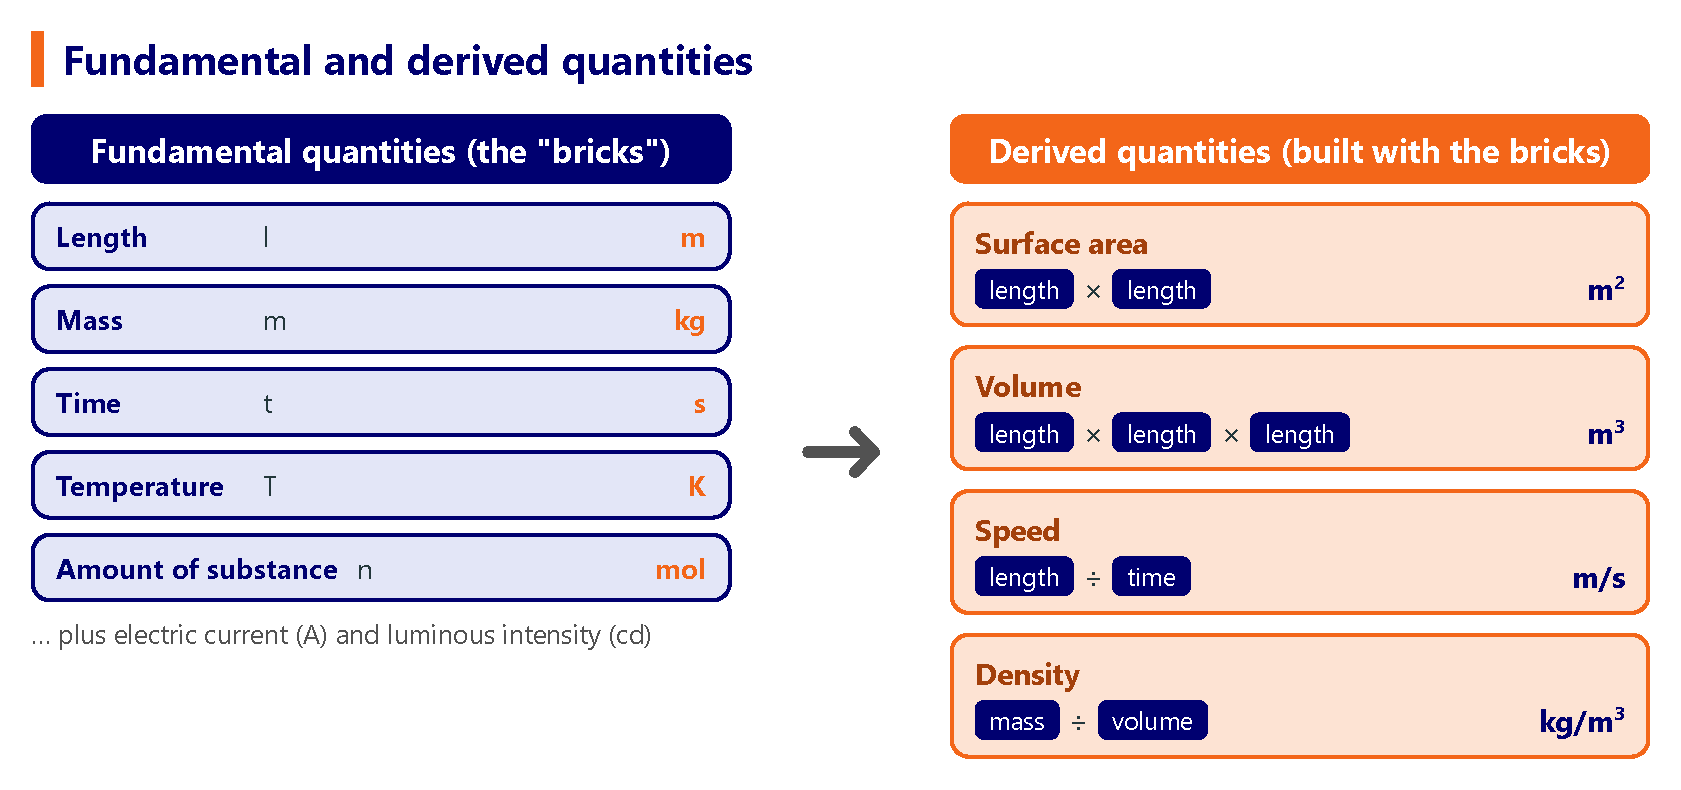
\includegraphics[width=\textwidth]{FigurasSVG/Unit_1_Matter_Measurement/pdf/fundamental_derived.pdf}
    \caption{Fundamental quantities are the ``bricks'' used to build derived quantities.}
    \label{fig:u1_fundamental_derived}
\end{figure}

\begin{table}[H]
    \centering
    \small
    \renewcommand{\arraystretch}{1.35}
    \begin{tabular}{p{2.6cm}cp{3.9cm}p{2.3cm}c}
        \toprule
        \textbf{Quantity} & \textbf{Symbol} & \textbf{Most used units} & \textbf{Unit symbols} & \textbf{SI unit} \\
        \midrule
        Length & \(l\) & kilometre, metre, centimetre, millimetre & \unit{\km}, \unit{\m}, \unit{\cm}, \unit{\mm} & metre (\unit{\m}) \\
        Mass & \(m\) & tonne, kilogram, gram, milligram & \unit{\tonne}, \unit{\kg}, \unit{\g}, \unit{\mg} & kilogram (\unit{\kg}) \\
        Time & \(t\) & day, hour, minute, second & \unit{\day}, \unit{\hour}, \unit{\minute}, \unit{\s} & second (\unit{\s}) \\
        Temperature & \(T\) & degree Celsius, kelvin & \unit{\celsius}, \unit{\K} & kelvin (\unit{\K}) \\
        Amount of substance & \(n\) & mole, millimole & \unit{\mol}, \unit{\milli\mol} & mole (\unit{\mol}) \\
        Electric current & \(I\) & ampere, milliampere & \unit{\A}, \unit{\mA} & ampere (\unit{\A}) \\
        Luminous intensity & \(I_{v}\) & candela & \unit{\candela} & candela (\unit{\candela}) \\
        \bottomrule
    \end{tabular}
    \caption{Fundamental quantities and their most used units.}
    \label{tab:u1_fundamental}
\end{table}

\begin{table}[H]
    \centering
    \small
    \renewcommand{\arraystretch}{1.35}
    \begin{tabular}{p{2.6cm}cp{3.9cm}p{2.3cm}c}
        \toprule
        \textbf{Quantity} & \textbf{Symbol} & \textbf{Most used units} & \textbf{Unit symbols} & \textbf{SI unit} \\
        \midrule
        Surface area \newline (length \(\times\) length) & \(S\) & square kilometre, hectare, square metre, square centimetre & \unit{\square\km}, \unit{\hectare}, \unit{\square\m}, \unit{\square\cm} & \unit{\square\m} \\
        Volume \newline (length\(^3\)) & \(V\) & cubic metre, cubic centimetre, litre, millilitre & \unit{\cubic\m}, \unit{\cubic\cm}, \unit{\litre}, \unit{\mL} & \unit{\cubic\m} \\
        Density \newline (mass \(\div\) volume) & \(d\) & kilogram per cubic metre, gram per millilitre, gram per litre & \unit{\kg\per\cubic\m}, \unit{\g\per\mL}, \unit{\g\per\litre} & \unit{\kg\per\cubic\m} \\
        Speed \newline (length \(\div\) time) & \(v\) & kilometre per hour, metre per second & \unit{\km\per\hour}, \unit{\m\per\s} & \unit{\m\per\s} \\
        Force & \(F\) & newton, kilopond & \unit{\N}, \unit{\kp} & newton (\unit{\N}) \\
        Pressure & \(p\) & pascal, atmosphere, millimetre of mercury & \unit{\Pa}, \unit{\atmospher}, \unit{\mmhg} & pascal (\unit{\Pa}) \\
        Energy & \(E\) & joule, calorie, kilocalorie, kilowatt-hour & \unit{\J}, \unit{\calorie}, \unit{\kilo\calorie}, \unit{\kwh} & joule (\unit{\J}) \\
        \bottomrule
    \end{tabular}
    \caption{Some derived quantities and their most used units.}
    \label{tab:u1_derived}
\end{table}

\begin{impt}
    Notice that the symbol of a \textbf{quantity} is written in \textit{italics} (\(m\), \(V\), \(t\)) and the symbol of a \textbf{unit} in upright letters (\unit{\m}, \unit{\litre}, \unit{\s}). Do not mix up \(m\) (the quantity \emph{mass}) with \unit{\m} (the unit \emph{metre}).
\end{impt}

\begin{exercise}
    Classify each quantity as \textbf{fundamental} or \textbf{derived}, and write its SI unit: mass, speed, time, surface area, temperature, density, length, volume.
    \begin{solu}
        \textbf{Fundamental}: mass (\unit{\kg}), time (\unit{\s}), temperature (\unit{\K}), length (\unit{\m}). \\
        \textbf{Derived}: speed (\unit{\m\per\s}), surface area (\unit{\square\m}), density (\unit{\kg\per\cubic\m}), volume (\unit{\cubic\m}).
    \end{solu}
\end{exercise}

\begin{exercise}
    The SI unit of density is \unit{\kg\per\cubic\m}. Explain, using the fundamental quantities, where this unit comes from.
    \begin{solu}
        Density is mass divided by volume, \(d = m/V\). Mass is measured in \unit{\kg}, and volume is length \(\times\) length \(\times\) length, so it is measured in \(\unit{\m}\cdot\unit{\m}\cdot\unit{\m} = \unit{\cubic\m}\). Dividing both units: \unit{\kg\per\cubic\m}.
    \end{solu}
\end{exercise}

%----------------------------------------------------------------------------------------

\subsection{Multiples and submultiples}

The objects we study can be tiny (a bacterium) or enormous (the Earth). If we always used the base unit, we would have to write numbers full of zeros, which are hard to read and easy to get wrong. To avoid this, the SI adds a \negsubro{prefix} in front of the unit.

\begin{definition}[Multiple and submultiple]
    A \textbf{multiple} is a unit bigger than the base unit (\unit{\km} is \(10^{3}\) times bigger than \unit{\m}). A \textbf{submultiple} is a unit smaller than the base unit (\unit{\mm} is \(10^{3}\) times smaller than \unit{\m}). Each one is named by adding a \textbf{prefix} to the base unit, and each prefix is worth a \textbf{power of 10}.
\end{definition}

\begin{figure}[H]
    \centering
    % [FIGURA ORIGINAL] \includegraphics[width=\textwidth]{Unit_1/prefix_scale}
    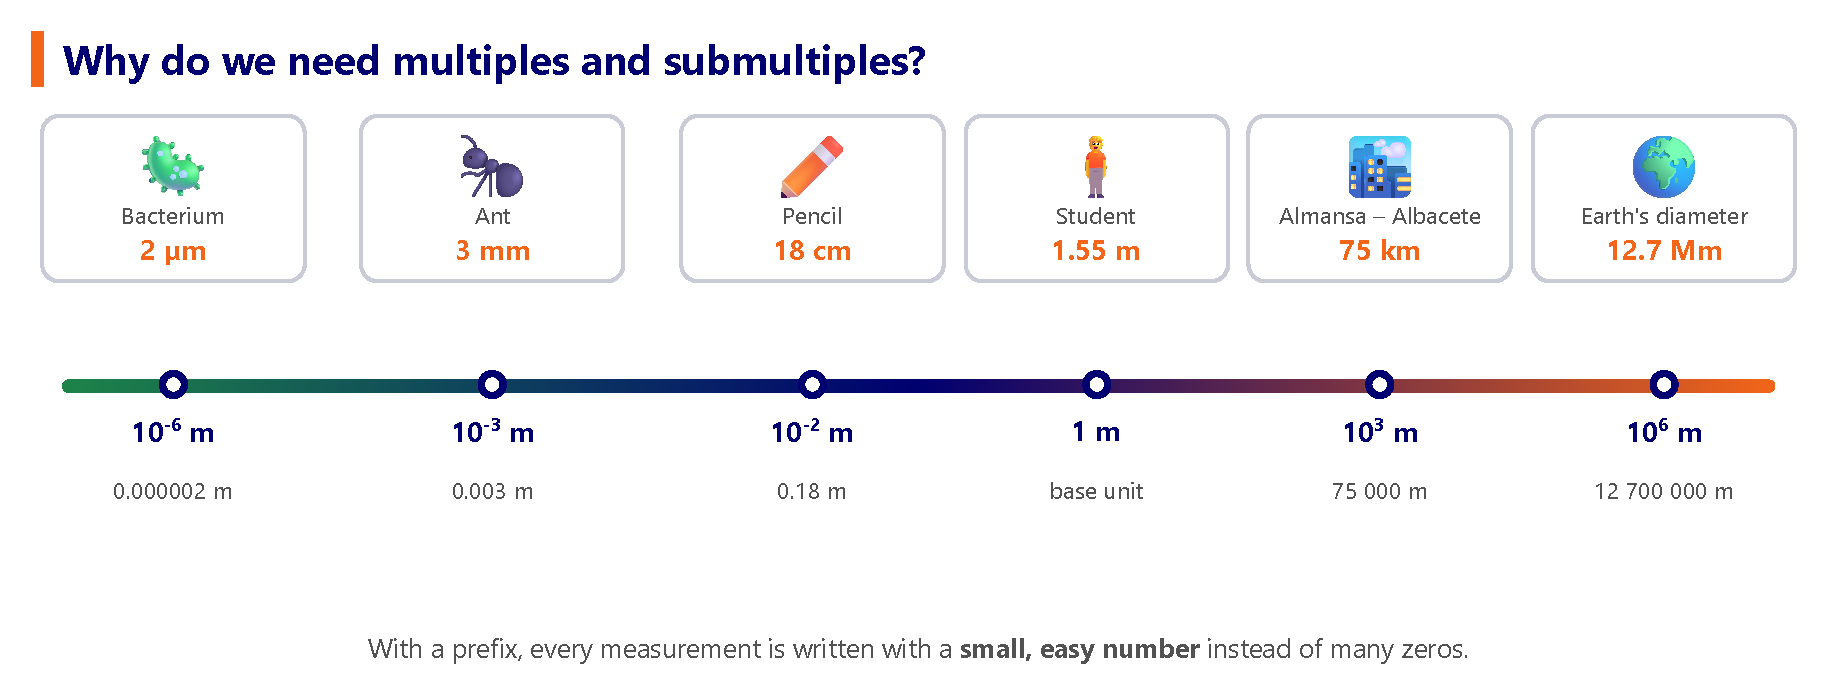
\includegraphics[width=\textwidth]{FigurasSVG/Unit_1_Matter_Measurement/pdf/prefix_scale.pdf}
    \caption{With prefixes, very small and very big lengths are written with simple numbers.}
    \label{fig:u1_prefix_scale}
\end{figure}

\begin{table}[H]
    \centering
    \small
    \renewcommand{\arraystretch}{1.3}
    \begin{tabular}{ccccrl}
        \toprule
         & \textbf{Prefix} & \textbf{Symbol} & \textbf{Power of 10} & \textbf{Decimal value} & \textbf{Example} \\
        \midrule
        \multirow{5}{*}{\rotatebox{90}{\textbf{Multiples}}}
         & giga & G & \(10^{9}\) & \num{1000000000} & \qty{1}{\giga\byte} (memory) \\
         & mega & M & \(10^{6}\) & \num{1000000} & \qty{1}{\mega\m} \\
         & kilo & k & \(10^{3}\) & \num{1000} & \qty{1}{\km}, \qty{1}{\kg} \\
         & hecto & h & \(10^{2}\) & \num{100} & \qty{1}{\hecto\litre} \\
         & deca & da & \(10^{1}\) & \num{10} & \qty{1}{\deca\gram} \\
        \midrule
        \multicolumn{3}{c}{\textbf{Base unit}} & \(10^{0}\) & \num{1} & \unit{\m}, \unit{\g}, \unit{\litre}, \unit{\s} \\
        \midrule
        \multirow{5}{*}{\rotatebox{90}{\textbf{Submultiples}}}
         & deci & d & \(10^{-1}\) & \num{0.1} & \qty{1}{\deci\litre} \\
         & centi & c & \(10^{-2}\) & \num{0.01} & \qty{1}{\cm} \\
         & milli & m & \(10^{-3}\) & \num{0.001} & \qty{1}{\mm}, \qty{1}{\mg} \\
         & micro & \(\upmu\) & \(10^{-6}\) & \num{0.000001} & \qty{1}{\um} (bacterium) \\
         & nano & n & \(10^{-9}\) & \num{0.000000001} & \qty{1}{\nm} (virus) \\
        \bottomrule
    \end{tabular}
    \caption{Multiples and submultiples of the units.}
    \label{tab:u1_prefixes}
\end{table}

\begin{impt}
    \negsubro{Why are multiples and submultiples so important?}
    \begin{itemize}
        \item They let us write any measurement with a \textbf{simple number}: \qty{75}{\km} is much clearer than \qty{75000}{\m}, and \qty{2}{\um} is much clearer than \qty{0.000002}{\m}.
        \item Since every prefix is a \textbf{power of 10}, changing from one to another is very easy: we only move the decimal point.
        \item The same prefixes work for \textbf{all} units: \unit{\km}, \unit{\kg}, \unit{\kilo\litre}, \unit{\kilo\joule}\ldots
    \end{itemize}
\end{impt}

The units of length, mass and capacity can be ordered as a staircase. Each step is worth \textbf{10}, so to know how many times a unit contains another one, we only have to \textbf{count the steps} between them.

\begin{figure}[H]
    \centering
    % [FIGURA ORIGINAL] \includegraphics[width=0.75\textwidth]{Unit_1/prefix_ladder}
    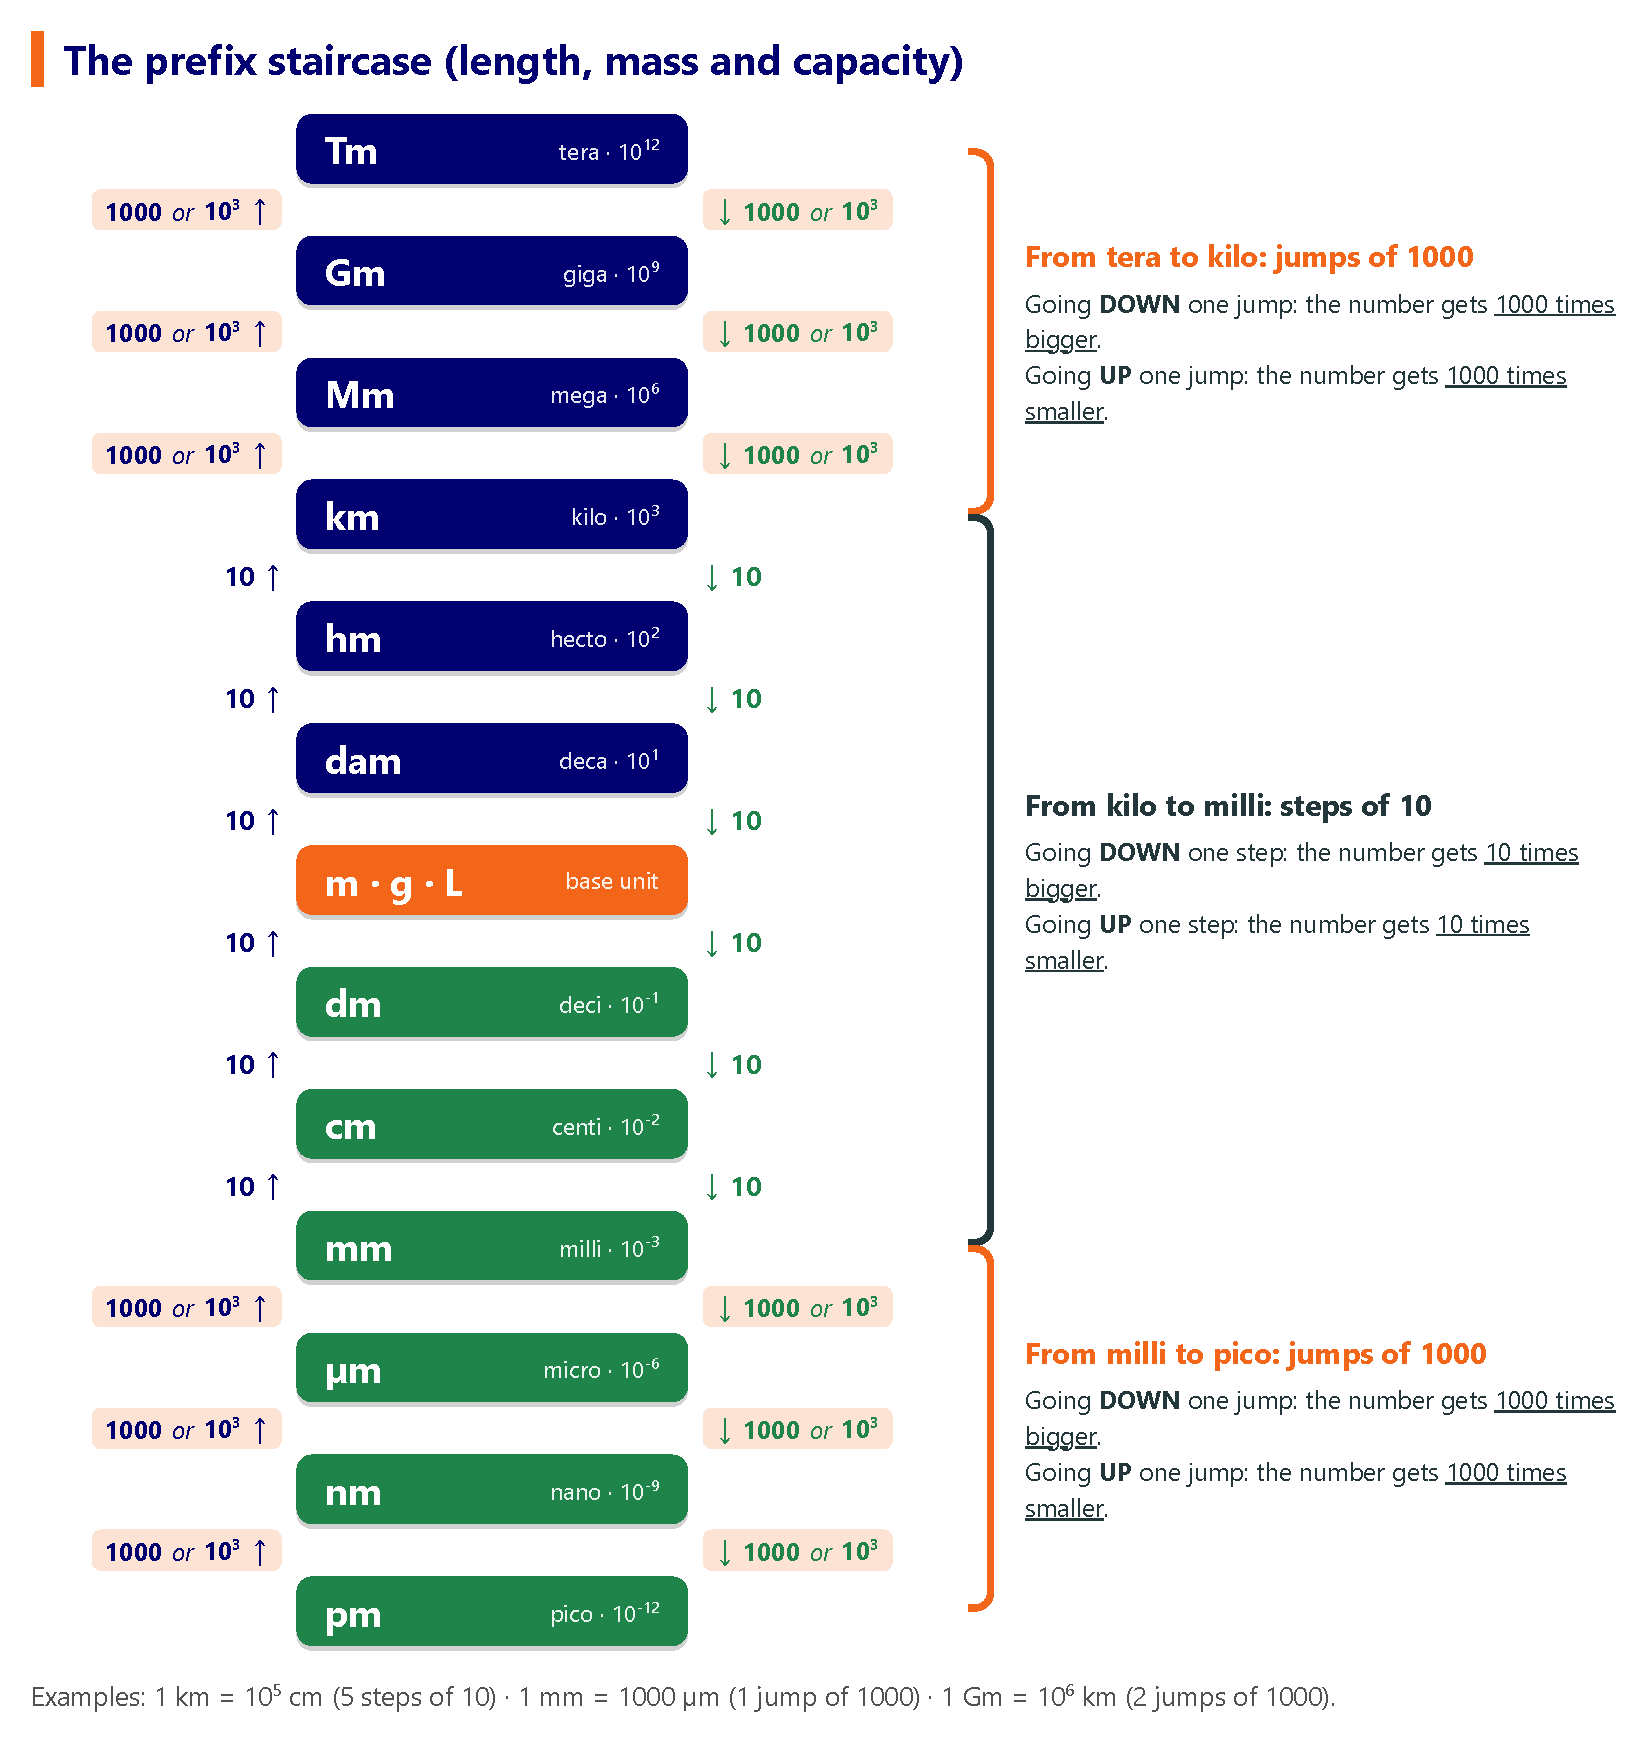
\includegraphics[width=0.75\textwidth]{FigurasSVG/Unit_1_Matter_Measurement/pdf/prefix_ladder.pdf}
    \caption{The prefix staircase: each step is a power of 10.}
    \label{fig:u1_prefix_ladder}
\end{figure}

\begin{example}
    Counting the steps on the staircase:
    \begin{itemize}
        \item From \unit{\km} to \unit{\m} there are 3 steps: \(\qty{1}{\km} = \qty{e3}{\m}\).
        \item From \unit{\m} to \unit{\cm} there are 2 steps: \(\qty{1}{\m} = \qty{e2}{\cm}\).
        \item From \unit{\kg} to \unit{\mg} there are 6 steps: \(\qty{1}{\kg} = \qty{e6}{\mg}\).
        \item From \unit{\deca\litre} to \unit{\centi\litre} there are 3 steps: \(\qty{1}{\deca\litre} = \qty{e3}{\centi\litre}\).
    \end{itemize}
\end{example}

\begin{exercise}
    Write the equivalence between each pair of units, putting the \textbf{1} in front of the bigger unit and using a power of 10: \textbf{a)} \unit{\hecto\m} and \unit{\dm}; \textbf{b)} \unit{\g} and \unit{\mg}; \textbf{c)} \unit{\kilo\litre} and \unit{\mL}; \textbf{d)} \unit{\cm} and \unit{\mm}; \textbf{e)} \unit{\deca\gram} and \unit{\deci\gram}.
    \begin{solu}
        a) \(\qty{1}{\hecto\m} = \qty{e3}{\dm}\); b) \(\qty{1}{\g} = \qty{e3}{\mg}\); c) \(\qty{1}{\kilo\litre} = \qty{e6}{\mL}\); d) \(\qty{1}{\cm} = \qty{e1}{\mm} = \qty{10}{\mm}\); e) \(\qty{1}{\deca\gram} = \qty{e2}{\deci\gram}\).
    \end{solu}
\end{exercise}

\begin{exercise}
    Choose the most suitable unit to express each measurement: the thickness of a coin, the distance from Almansa to Madrid, the mass of a lorry, the mass of a grain of rice, the volume of water in a swimming pool, the volume of a medicine dose.
    \begin{solu}
        Thickness of a coin: \unit{\mm}. Distance Almansa--Madrid: \unit{\km}. Mass of a lorry: \unit{\tonne} or \unit{\kg}. Mass of a grain of rice: \unit{\mg}. Water in a pool: \unit{\cubic\m} or \unit{\kilo\litre}. Medicine dose: \unit{\mL}.
    \end{solu}
\end{exercise}

\begin{impt}
    \negsubro{How to read a unit (very important!)}

    When we look at a unit, we always read it \textbf{from right to left}:
    \begin{enumerate}[label=\numberballmDarkTeal]
        \item First we find the \textbf{symbol of the unit}: it is the \textbf{last} letter (or letters) of the symbol.
        \item Then we identify the \textbf{quantity} that the unit measures: \unit{\m} \(\to\) length, \unit{\g} \(\to\) mass, \unit{\litre} \(\to\) capacity, \unit{\s} \(\to\) time\ldots
        \item Finally, we look at the letter \textbf{in front of the unit}: it is the \textbf{prefix}, and it tells us whether it is a \textbf{multiple} or a \textbf{submultiple}. If there is no letter in front, it is the base unit.
    \end{enumerate}
\end{impt}

\begin{figure}[H]
    \centering
    % [FIGURA ORIGINAL] \includegraphics[width=\textwidth]{Unit_1/read_unit}
    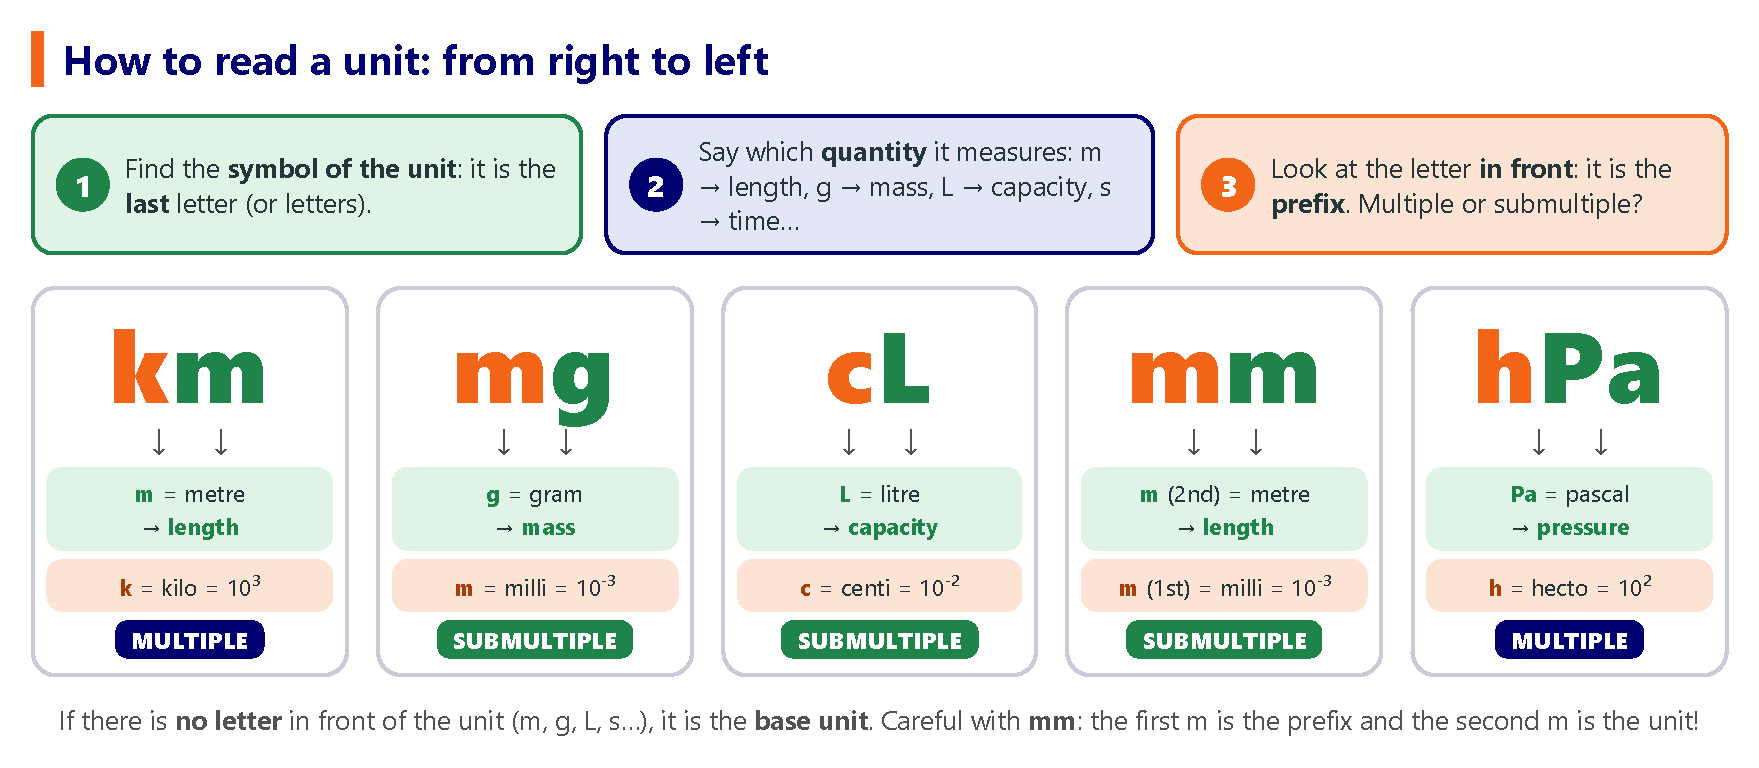
\includegraphics[width=\textwidth]{FigurasSVG/Unit_1_Matter_Measurement/pdf/read_unit.pdf}
    \caption{Reading a unit from right to left: first the unit and its quantity, then the prefix.}
    \label{fig:u1_read_unit}
\end{figure}

\begin{exercise}
    For each unit, say which quantity it measures, which prefix it has and whether it is a multiple or a submultiple: \unit{\kg}, \unit{\mL}, \unit{\cm}, \unit{\hecto\litre}, \unit{\ms}, \unit{\mm}.
    \begin{solu}
        \unit{\kg}: mass, kilo, multiple. \unit{\mL}: capacity, milli, submultiple. \unit{\cm}: length, centi, submultiple. \unit{\hecto\litre}: capacity, hecto, multiple. \unit{\ms}: time, milli, submultiple. \unit{\mm}: length, milli (the first m), submultiple.
    \end{solu}
\end{exercise}

%----------------------------------------------------------------------------------------

\subsection{Changing units: conversion factors}

Very often we need to express a measurement in a different unit: a recipe in grams when our scale uses kilograms, or a speed in \unit{\m\per\s} when the car shows \unit{\km\per\hour}. In this book we will always change units with \negsubro{conversion factors}.

\begin{impt}
    \negsubro{What does ``changing units'' mean?}
    \begin{itemize}
        \item A change of units is a change between \textbf{different units of the same quantity}: \unit{\hour}, \unit{\minute} and \unit{\s} are all units of \textbf{time}, so we can change from one to another.
        \item It is also a change between \textbf{multiples and submultiples} of the same unit: \unit{\km} \(\to\) \unit{\m} \(\to\) \unit{\cm}.
        \item We can \textbf{never} change between units of \textbf{different quantities}: \unit{\km} can never become \unit{\kg}, because length and mass are different quantities.
    \end{itemize}
    The measurement does not change: it is the \textbf{same amount}, only written with a different unit.
\end{impt}

\begin{figure}[H]
    \centering
    % [FIGURA ORIGINAL] \includegraphics[width=\textwidth]{Unit_1/same_quantity}
    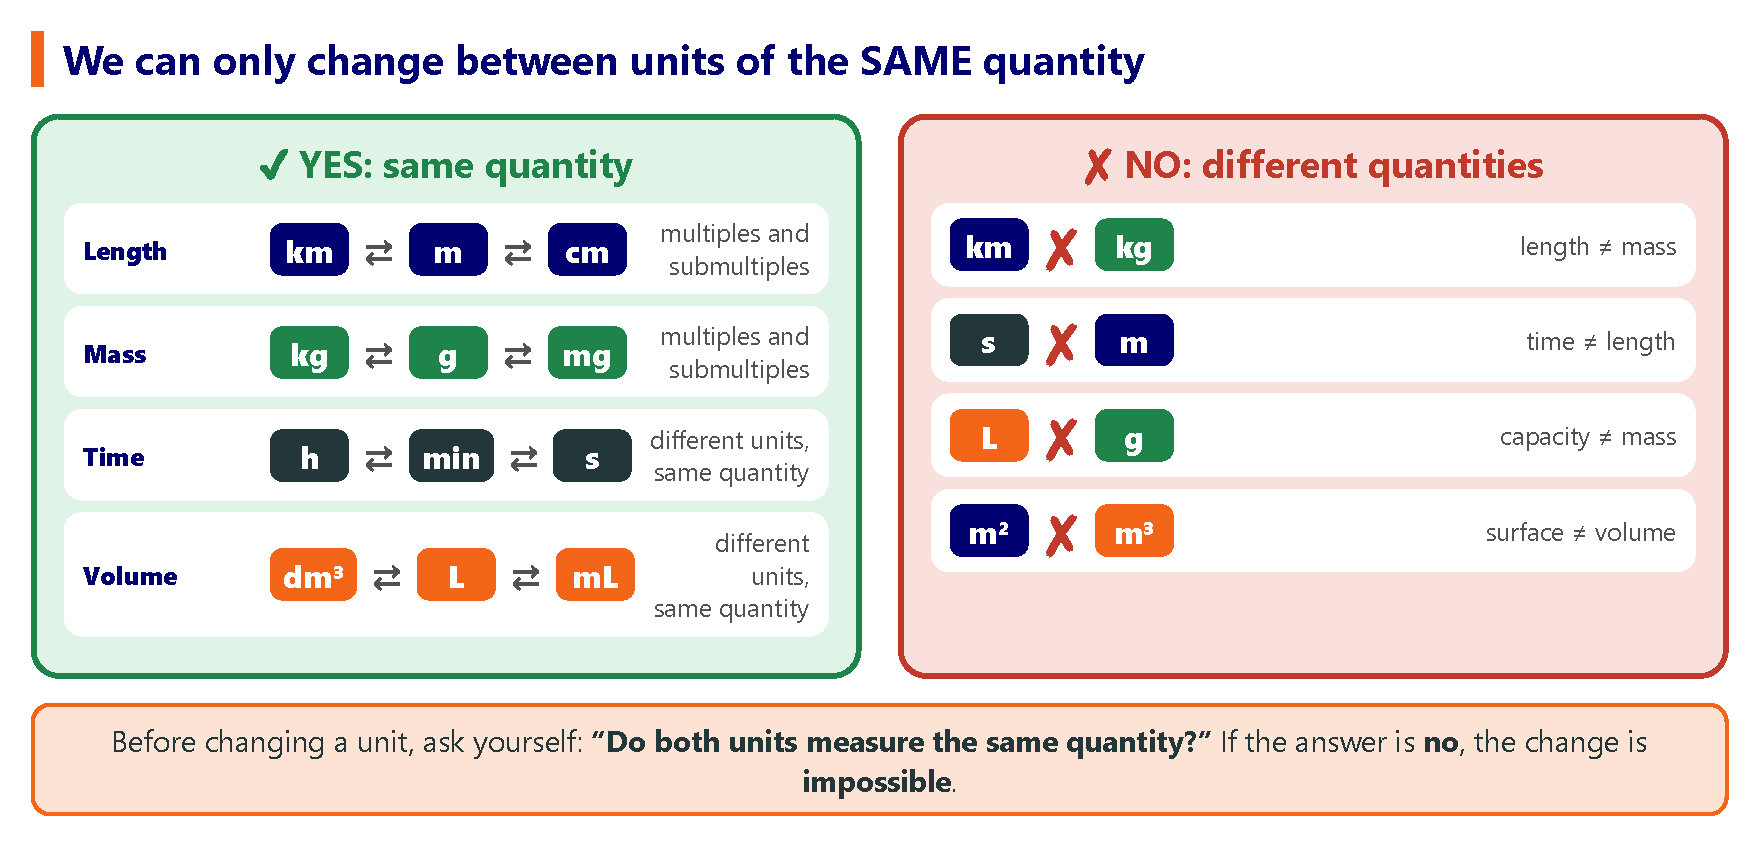
\includegraphics[width=\textwidth]{FigurasSVG/Unit_1_Matter_Measurement/pdf/same_quantity.pdf}
    \caption{We can only change between units that measure the same quantity.}
    \label{fig:u1_same_quantity}
\end{figure}

\begin{definition}[Conversion factor]
    A fraction whose numerator and denominator are the \textbf{same amount}, written in \textbf{different units}. For example,
    \(\dfrac{\qty{e3}{\m}}{\qty{1}{\km}}\) or \(\dfrac{\qty{1}{\km}}{\qty{e3}{\m}}\).
    Since the top and the bottom are equal, a conversion factor is worth exactly \textbf{1}: multiplying by it does not change the quantity, only the unit in which it is written.
\end{definition}

\begin{impt}
    \negsubro{Golden rules for writing conversion factors}
    \begin{enumerate}[label=\numberballmDarkTeal]
        \item In the equivalence between the two units, the \textbf{1} always goes with the \textbf{bigger unit}: \(\qty{1}{\km} = \qty{e3}{\m}\) (never \(\qty{1}{\m} = \qty{e-3}{\km}\)); \(\qty{1}{\hour} = \qty{3600}{\s}\); \(\qty{1}{\atmospher} = \qty{760}{\mmhg}\).
        \item Between multiples and submultiples, and whenever the numbers are very big, we always use \textbf{powers of 10}: \(\qty{1}{\kg} = \qty{e6}{\mg}\) instead of \(\qty{1}{\kg} = \qty{1000000}{\mg}\).
        \item The unit we want to \textbf{remove} goes in the \textbf{denominator}, and the unit we want to \textbf{obtain} goes in the \textbf{numerator}.
    \end{enumerate}
\end{impt}

\begin{figure}[H]
    \centering
    % [FIGURA ORIGINAL] \includegraphics[width=0.95\textwidth]{Unit_1/conversion_factor}
    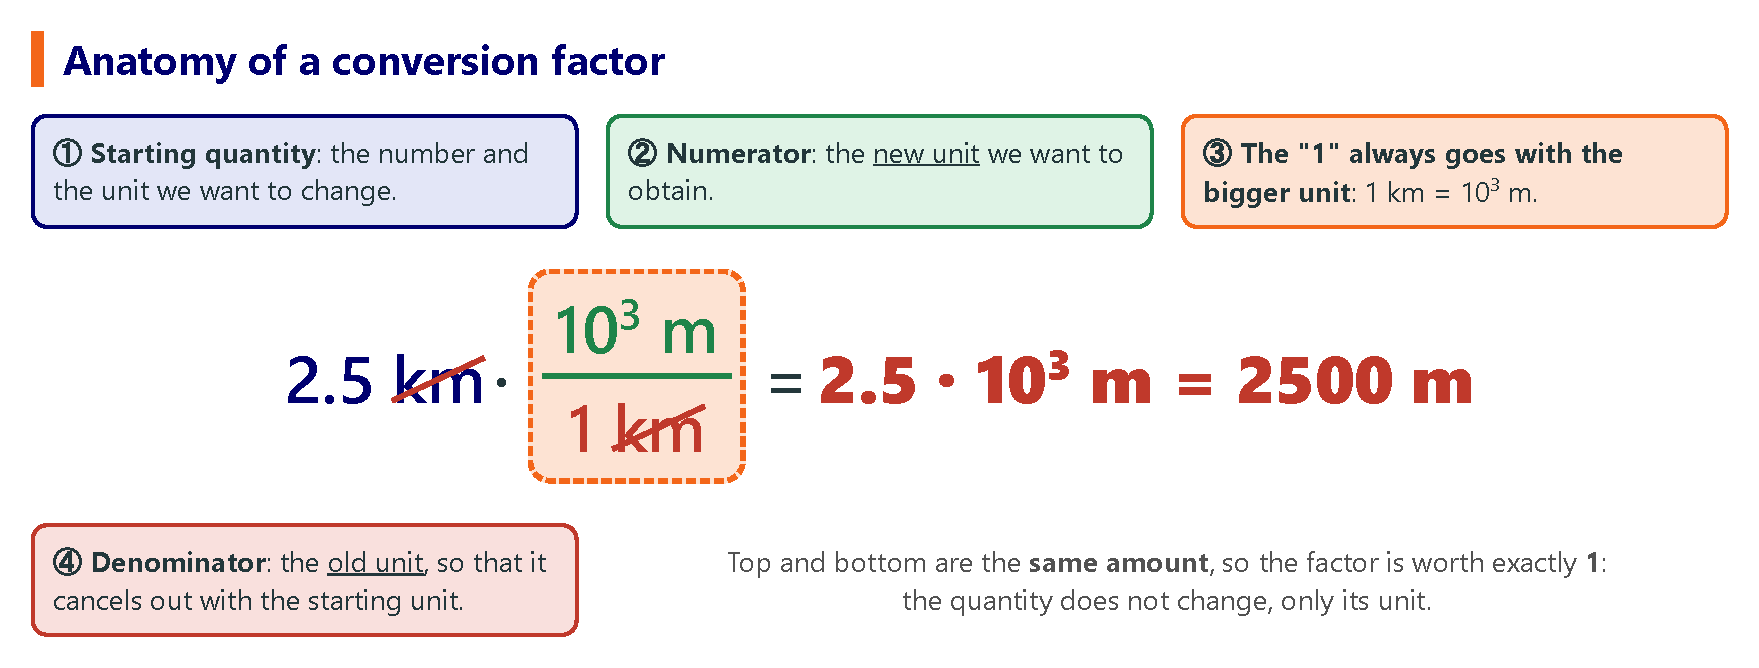
\includegraphics[width=0.95\textwidth]{FigurasSVG/Unit_1_Matter_Measurement/pdf/conversion_factor.pdf}
    \caption{The parts of a conversion factor.}
    \label{fig:u1_conversion_factor}
\end{figure}

\negsubro{Method, step by step}:
\begin{enumerate}[label=\numberballmDarkTeal]
    \item Write the quantity you want to change (number and unit).
    \item Write the \textbf{equivalence} between the initial unit and the final unit, with the 1 in front of the bigger unit and using powers of 10.
    \item Build the \textbf{conversion factor} from the equivalence: the initial unit goes in the denominator, so that it cancels out, and the final unit goes in the numerator.
    \item Multiply, \textbf{cancel} the units that appear above and below, and calculate.
    \item Write the result with its unit (if it has many zeros, leave it as a power of 10).
\end{enumerate}

If there is no direct equivalence between the two units, we can link several conversion factors one after the other, like the links of a chain.

%------------------------------------------------

\subsubsection{Simple units: length, mass and capacity}

\begin{example}
    \textbf{Write \qty{0.8}{\km} in \unit{\dm}.}
    \begin{enumerate}[label=\numberballmDarkTeal]
        \item Quantity: \qty{0.8}{\km}.
        \item Equivalence (4 steps on the staircase, the 1 goes with \unit{\km}): \(\qty{1}{\km} = \qty{e4}{\dm}\).
        \item The unit to remove (\unit{\km}) goes in the denominator.
        \item \(
            \num{0.8}\,\cancelunit{\km} \cdot \dfrac{\qty{e4}{\dm}}{1\,\cancelunit{\km}} = \qty{0.8e4}{\dm}
        \)
        \item \(\textcolor{red}{\qty{8000}{\dm}}\)
    \end{enumerate}
\end{example}

\begin{example}
    \textbf{Write \qty{850}{\deci\gram} in \unit{\hecto\gram}.} \\
    Equivalence (3 steps, the 1 goes with \unit{\hecto\gram}, which is bigger): \(\qty{1}{\hecto\gram} = \qty{e3}{\deci\gram}\).
    \begin{equation*}
        \num{850}\,\cancelunit{\deci\gram} \cdot \dfrac{\qty{1}{\hecto\gram}}{\num{e3}\,\cancelunit{\deci\gram}} = \qty{850e-3}{\hecto\gram} = \textcolor{red}{\qty{0.85}{\hecto\gram}}
    \end{equation*}
\end{example}

\begin{example}
    \textbf{Write \qty{2.5}{\litre} in \unit{\mL}.} \\
    Equivalence: \(\qty{1}{\litre} = \qty{e3}{\mL}\).
    \begin{equation*}
        \num{2.5}\,\cancelunit{\litre} \cdot \dfrac{\qty{e3}{\mL}}{1\,\cancelunit{\litre}} = \qty{2.5e3}{\mL} = \textcolor{red}{\qty{2500}{\mL}}
    \end{equation*}
\end{example}

\begin{exercise}
    Convert these amounts using conversion factors:
    \begin{enumerate}[label=\letraminuscula]
        \item \(\qty{25.8}{\g} \to \unit{\centi\gram}\)
        \item \(\qty{0.05}{\hecto\gram} \to \unit{\deci\gram}\)
        \item \(\qty{3.5}{\deca\gram} \to \unit{\kg}\)
        \item \(\qty{450}{\mg} \to \unit{\kg}\)
        \item \(\qty{1.2}{\km} \to \unit{\cm}\)
        \item \(\qty{330}{\mL} \to \unit{\litre}\)
    \end{enumerate}
    \begin{solu}
        \begin{enumerate}[label=\alph*)]
            \item \(\num{25.8}\,\unit{\g} \cdot \dfrac{\qty{e2}{\centi\gram}}{\qty{1}{\g}} = \qty{2580}{\centi\gram}\)
            \item \(\num{0.05}\,\unit{\hecto\gram} \cdot \dfrac{\qty{e3}{\deci\gram}}{\qty{1}{\hecto\gram}} = \qty{50}{\deci\gram}\)
            \item \(\num{3.5}\,\unit{\deca\gram} \cdot \dfrac{\qty{1}{\kg}}{\qty{e2}{\deca\gram}} = \qty{3.5e-2}{\kg} = \qty{0.035}{\kg}\)
            \item \(\num{450}\,\unit{\mg} \cdot \dfrac{\qty{1}{\kg}}{\qty{e6}{\mg}} = \qty{4.5e-4}{\kg} = \qty{0.00045}{\kg}\)
            \item \(\num{1.2}\,\unit{\km} \cdot \dfrac{\qty{e5}{\cm}}{\qty{1}{\km}} = \qty{1.2e5}{\cm} = \qty{120000}{\cm}\)
            \item \(\num{330}\,\unit{\mL} \cdot \dfrac{\qty{1}{\litre}}{\qty{e3}{\mL}} = \qty{0.33}{\litre}\)
        \end{enumerate}
    \end{solu}
\end{exercise}

\begin{exercise}
    Order these amounts from largest to smallest: \qty{0.015}{\kg}, \qty{2765}{\deci\gram}, \qty{2.54}{\deca\gram}.
    \begin{solu}
        We change all of them to grams: \\
        \(\num{0.015}\,\unit{\kg} \cdot \dfrac{\qty{e3}{\g}}{\qty{1}{\kg}} = \qty{15}{\g}\); \quad
        \(\num{2765}\,\unit{\deci\gram} \cdot \dfrac{\qty{1}{\g}}{\qty{e1}{\deci\gram}} = \qty{276.5}{\g}\); \quad
        \(\num{2.54}\,\unit{\deca\gram} \cdot \dfrac{\qty{e1}{\g}}{\qty{1}{\deca\gram}} = \qty{25.4}{\g}\). \\
        Order: \(\qty{2765}{\deci\gram} > \qty{2.54}{\deca\gram} > \qty{0.015}{\kg}\).
    \end{solu}
\end{exercise}

\begin{exercise}
    A recipe needs \qty{0.75}{\kg} of flour, but the kitchen scale only shows grams. How many grams should be weighed? If a bag contains \qty{2}{\kg} of flour, how many complete recipes can be made with it?
    \begin{solu}
        \(\num{0.75}\,\unit{\kg} \cdot \dfrac{\qty{e3}{\g}}{\qty{1}{\kg}} = \qty{750}{\g}\). \\
        \(\qty{2}{\kg} = \qty{2000}{\g}\); number of recipes \(= 2000 / 750 \approx \num{2.67}\), so \textbf{2 complete recipes} can be made.
    \end{solu}
\end{exercise}

\begin{exercise}
    Convert these amounts using conversion factors:
    \begin{enumerate}[label=\letraminuscula]
        \item \(\qty{500}{\hecto\gram} \to \unit{\g}\)
        \item \(\qty{60}{\cm} \to \unit{\m}\)
        \item \(\qty{2000}{\hecto\m} \to \unit{\deca\m}\)
        \item \(\qty{5.7}{\kg} \to \unit{\g}\)
        \item \(\qty{300}{\dm} \to \unit{\hecto\m}\)
        \item \(\qty{563}{\km} \to \unit{\hecto\m}\)
        \item \(\qty{3}{\dm} \to \unit{\deca\m}\)
        \item \(\qty{7}{\dm} \to \unit{\cm}\)
        \item \(\qty{5}{\giga\m} \to \unit{\nano\m}\)
        \item \(\qty{26}{\micro\m} \to \unit{\km}\)
    \end{enumerate}
    \begin{solu}
        \begin{enumerate}[label=\alph*)]
            \item \(\num{500}\,\unit{\hecto\gram} \cdot \dfrac{\qty{e2}{\g}}{\qty{1}{\hecto\gram}} = \qty{5e4}{\g} = \qty{50000}{\g}\)
            \item \(\num{60}\,\unit{\cm} \cdot \dfrac{\qty{1}{\m}}{\qty{e2}{\cm}} = \qty{0.6}{\m}\)
            \item \(\num{2000}\,\unit{\hecto\m} \cdot \dfrac{\qty{e1}{\deca\m}}{\qty{1}{\hecto\m}} = \qty{2e4}{\deca\m}\)
            \item \(\num{5.7}\,\unit{\kg} \cdot \dfrac{\qty{e3}{\g}}{\qty{1}{\kg}} = \qty{5.7e3}{\g} = \qty{5700}{\g}\)
            \item \(\num{300}\,\unit{\dm} \cdot \dfrac{\qty{1}{\hecto\m}}{\qty{e3}{\dm}} = \qty{0.3}{\hecto\m}\)
            \item \(\num{563}\,\unit{\km} \cdot \dfrac{\qty{e1}{\hecto\m}}{\qty{1}{\km}} = \qty{5630}{\hecto\m}\)
            \item \(\num{3}\,\unit{\dm} \cdot \dfrac{\qty{1}{\deca\m}}{\qty{e2}{\dm}} = \qty{3e-2}{\deca\m} = \qty{0.03}{\deca\m}\)
            \item \(\num{7}\,\unit{\dm} \cdot \dfrac{\qty{e1}{\cm}}{\qty{1}{\dm}} = \qty{70}{\cm}\)
            \item \(\num{5}\,\unit{\giga\m} \cdot \dfrac{\qty{e9}{\m}}{\qty{1}{\giga\m}} \cdot \dfrac{\qty{e9}{\nano\m}}{\qty{1}{\m}} = \qty{5e18}{\nano\m}\)
            \item \(\num{26}\,\unit{\micro\m} \cdot \dfrac{\qty{1}{\m}}{\qty{e6}{\micro\m}} \cdot \dfrac{\qty{1}{\km}}{\qty{e3}{\m}} = \qty{26e-9}{\km} = \qty{2.6e-8}{\km}\)
        \end{enumerate}
    \end{solu}
\end{exercise}

%------------------------------------------------

\subsubsection{Surface area}

\begin{definition}[Surface area]
    A quantity obtained by multiplying two lengths, expressed in the same unit. Its SI unit is the square metre, \unit{\square\metre}.
\end{definition}

\begin{equation*}
    \qty{5.40}{\m} \cdot \qty{6.50}{\m} = \qty{35.10}{\square\metre}
\end{equation*}

A square of \qty{1}{\m} \(\times\) \qty{1}{\m} can be divided into \(10 \times 10 = 100\) small squares of \qty{1}{\dm} \(\times\) \qty{1}{\dm}. So, while \(\qty{1}{\m} = \qty{10}{\dm}\), we have \(\qty{1}{\square\m} = \qty{e2}{\square\dm}\): \textbf{the factor of length is squared}.

\begin{figure}[H]
    \centering
    % [FIGURA ORIGINAL] \includegraphics[width=0.85\textwidth]{Unit_1/square_units}
    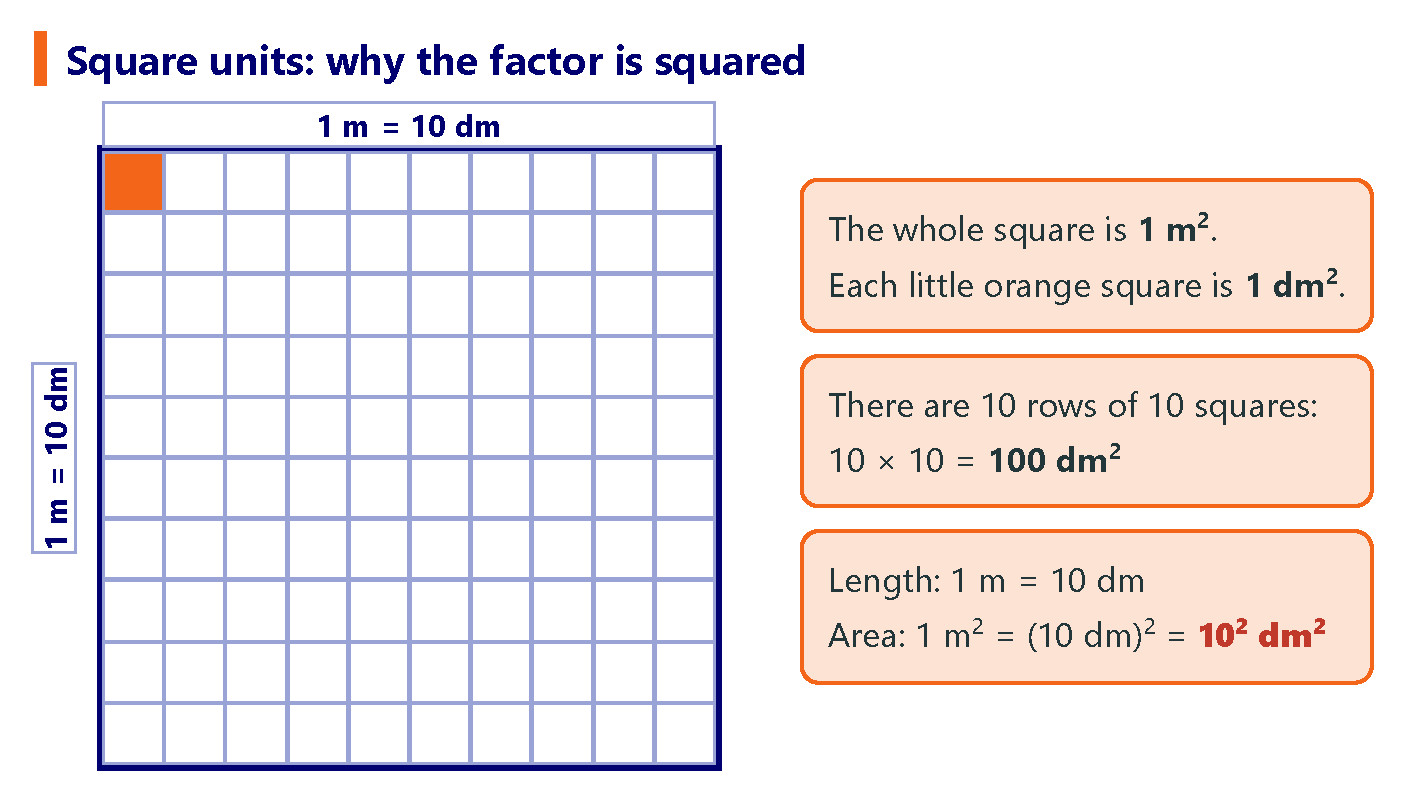
\includegraphics[width=0.85\textwidth]{FigurasSVG/Unit_1_Matter_Measurement/pdf/square_units.pdf}
    \caption{One square metre contains \(10^{2}\) square decimetres.}
    \label{fig:u1_square_units}
\end{figure}

\begin{impt}
    \negsubro{Trick for surface area}: write the conversion factor as if it were a change of \textbf{length} (a simple unit), and then \textbf{raise the whole factor to the power of 2}.
    \begin{equation*}
        \text{Length: } \dfrac{\qty{e2}{\cm}}{\qty{1}{\m}}
        \quad\Longrightarrow\quad
        \text{Surface: } \left(\dfrac{\qty{e2}{\cm}}{\qty{1}{\m}}\right)^{2} = \dfrac{\qty{e4}{\square\cm}}{\qty{1}{\square\m}}
    \end{equation*}
    Each step on the staircase of surface units is therefore worth \(10^{2} = 100\).
\end{impt}

\begin{table}[H]
    \centering
    \small
    \renewcommand{\arraystretch}{1.3}
    \begin{tabular}{cccc}
        \toprule
        \textbf{Unit} & \textbf{Symbol} & \textbf{Equivalence with \unit{\square\m}} & \textbf{Equivalent length} \\
        \midrule
        square kilometre & \unit{\square\km} & \(\qty{1}{\square\km} = \qty{e6}{\square\m}\) & \(\qty{1}{\km} = \qty{e3}{\m}\) \\
        square hectometre (hectare) & \unit{\square\hecto\m} (\unit{\hectare}) & \(\qty{1}{\square\hecto\m} = \qty{e4}{\square\m}\) & \(\qty{1}{\hecto\m} = \qty{e2}{\m}\) \\
        square decametre & \unit{\square\deca\m} & \(\qty{1}{\square\deca\m} = \qty{e2}{\square\m}\) & \(\qty{1}{\deca\m} = \qty{e1}{\m}\) \\
        \midrule
        square metre & \unit{\square\m} & base unit & base unit \\
        \midrule
        square decimetre & \unit{\square\dm} & \(\qty{1}{\square\m} = \qty{e2}{\square\dm}\) & \(\qty{1}{\m} = \qty{e1}{\dm}\) \\
        square centimetre & \unit{\square\cm} & \(\qty{1}{\square\m} = \qty{e4}{\square\cm}\) & \(\qty{1}{\m} = \qty{e2}{\cm}\) \\
        square millimetre & \unit{\square\mm} & \(\qty{1}{\square\m} = \qty{e6}{\square\mm}\) & \(\qty{1}{\m} = \qty{e3}{\mm}\) \\
        \bottomrule
    \end{tabular}
    \caption{Units of surface area.}
    \label{tab:u1_surface_units}
\end{table}

\begin{example}
    \textbf{Write \qty{0.5}{\square\deca\metre} in \unit{\square\dm}.}
    \begin{enumerate}[label=\numberballmDarkTeal]
        \item Simple change (length): \(\qty{1}{\deca\m} = \qty{e2}{\dm}\) \(\to\) factor \(\dfrac{\qty{e2}{\dm}}{\qty{1}{\deca\m}}\).
        \item We square it: \(\left(\dfrac{\qty{e2}{\dm}}{\qty{1}{\deca\m}}\right)^{2} = \dfrac{\qty{e4}{\square\dm}}{\qty{1}{\square\deca\m}}\).
        \item \(
            \num{0.5}\,\cancelunit{\square\deca\m} \cdot \dfrac{\qty{e4}{\square\dm}}{1\,\cancelunit{\square\deca\m}} = \qty{0.5e4}{\square\dm} = \textcolor{red}{\qty{5000}{\square\dm}}
        \)
    \end{enumerate}
\end{example}

\begin{example}
    \textbf{Write \qty{85}{\square\cm} in \unit{\square\m}.} \\
    Simple change: \(\qty{1}{\m} = \qty{e2}{\cm}\). Squaring the factor:
    \begin{equation*}
        \num{85}\,\cancelunit{\square\cm} \cdot \left(\dfrac{\qty{1}{\m}}{\num{e2}\,\cancelunit{\cm}}\right)^{2}
        = \num{85}\,\cancelunit{\square\cm} \cdot \dfrac{\qty{1}{\square\m}}{\num{e4}\,\cancelunit{\square\cm}}
        = \qty{85e-4}{\square\m} = \textcolor{red}{\qty{8.5e-3}{\square\m}}
    \end{equation*}
\end{example}

\begin{exercise}
    Convert these amounts using conversion factors:
    \begin{enumerate}[label=\letraminuscula]
        \item \(\qty{1.25}{\square\m} \to \unit{\square\cm}\)
        \item \(\qty{0.082}{\square\km} \to \unit{\square\dm}\)
        \item \(\qty{1.007}{\square\deca\metre} \to \unit{\square\mm}\)
        \item \(\qty{3500}{\square\mm} \to \unit{\square\dm}\)
    \end{enumerate}
    \begin{solu}
        \begin{enumerate}[label=\alph*)]
            \item \(\num{1.25}\,\unit{\square\m} \cdot \left(\dfrac{\qty{e2}{\cm}}{\qty{1}{\m}}\right)^{2} = \num{1.25}\,\unit{\square\m} \cdot \dfrac{\qty{e4}{\square\cm}}{\qty{1}{\square\m}} = \qty{1.25e4}{\square\cm} = \qty{12500}{\square\cm}\)
            \item \(\num{0.082}\,\unit{\square\km} \cdot \left(\dfrac{\qty{e4}{\dm}}{\qty{1}{\km}}\right)^{2} = \num{0.082}\,\unit{\square\km} \cdot \dfrac{\qty{e8}{\square\dm}}{\qty{1}{\square\km}} = \qty{8.2e6}{\square\dm}\)
            \item \(\num{1.007}\,\unit{\square\deca\m} \cdot \left(\dfrac{\qty{e4}{\mm}}{\qty{1}{\deca\m}}\right)^{2} = \num{1.007}\,\unit{\square\deca\m} \cdot \dfrac{\qty{e8}{\square\mm}}{\qty{1}{\square\deca\m}} = \qty{1.007e8}{\square\mm}\)
            \item \(\num{3500}\,\unit{\square\mm} \cdot \left(\dfrac{\qty{1}{\dm}}{\qty{e2}{\mm}}\right)^{2} = \num{3500}\,\unit{\square\mm} \cdot \dfrac{\qty{1}{\square\dm}}{\qty{e4}{\square\mm}} = \qty{0.35}{\square\dm}\)
        \end{enumerate}
    \end{solu}
\end{exercise}

\begin{exercise}
    A hectare (\unit{\hectare}) is the same as \qty{1}{\square\hecto\m}, that is, \qty{e4}{\square\m}. How many hectares is a football pitch that is \qty{100}{\m} long and \qty{70}{\m} wide?
    \begin{solu}
        Area \(= \qty{100}{\m} \cdot \qty{70}{\m} = \qty{7000}{\square\m}\). \\
        \(\num{7000}\,\unit{\square\m} \cdot \dfrac{\qty{1}{\hectare}}{\qty{e4}{\square\m}} = \qty{0.7}{\hectare}\).
    \end{solu}
\end{exercise}

\begin{exercise}
    A classroom floor measures \qty{8}{\m} by \qty{6}{\m}, and it is going to be covered with square tiles of \qty{400}{\square\cm} each. How many tiles are needed?
    \begin{solu}
        Floor area: \(\qty{8}{\m} \cdot \qty{6}{\m} = \qty{48}{\square\m}\). \\
        \(\num{48}\,\unit{\square\m} \cdot \left(\dfrac{\qty{e2}{\cm}}{\qty{1}{\m}}\right)^{2} = \num{48}\,\unit{\square\m} \cdot \dfrac{\qty{e4}{\square\cm}}{\qty{1}{\square\m}} = \qty{4.8e5}{\square\cm}\). \\
        Number of tiles: \(\num{480000} / \num{400} = \num{1200}\) tiles.
    \end{solu}
\end{exercise}

\begin{exercise}
    Convert these amounts using conversion factors:
    \begin{enumerate}[label=\letraminuscula]
        \item \(\qty{40}{\square\cm} \to \unit{\square\dm}\)
        \item \(\qty{3}{\square\hecto\m} \to \unit{\square\dm}\)
        \item \(\qty{50}{\square\cm} \to \unit{\square\m}\)
        \item \(\qty{0.02}{\square\dm} \to \unit{\square\deca\m}\)
        \item \(\qty{5}{\square\cm} \to \unit{\square\m}\)
        \item \(\qty{300}{\square\hecto\m} \to \unit{\square\dm}\)
        \item \(\qty{653}{\square\cm} \to \unit{\square\m}\)
        \item \(\qty{3}{\square\dm} \to \unit{\square\deca\m}\)
        \item \(\qty{1.5}{\square\hecto\m} \to \unit{\square\mm}\)
        \item \(\qty{5}{\square\giga\m} \to \unit{\square\nano\m}\)
        \item \(\qty{26}{\square\micro\m} \to \unit{\square\km}\)
    \end{enumerate}
    \begin{solu}
        \begin{enumerate}[label=\alph*)]
            \item \(\num{40}\,\unit{\square\cm} \cdot \left(\dfrac{\qty{1}{\dm}}{\qty{e1}{\cm}}\right)^{2} = \num{40}\,\unit{\square\cm} \cdot \dfrac{\qty{1}{\square\dm}}{\qty{e2}{\square\cm}} = \qty{0.4}{\square\dm}\)
            \item \(\num{3}\,\unit{\square\hecto\m} \cdot \left(\dfrac{\qty{e3}{\dm}}{\qty{1}{\hecto\m}}\right)^{2} = \num{3}\,\unit{\square\hecto\m} \cdot \dfrac{\qty{e6}{\square\dm}}{\qty{1}{\square\hecto\m}} = \qty{3e6}{\square\dm}\)
            \item \(\num{50}\,\unit{\square\cm} \cdot \left(\dfrac{\qty{1}{\m}}{\qty{e2}{\cm}}\right)^{2} = \num{50}\,\unit{\square\cm} \cdot \dfrac{\qty{1}{\square\m}}{\qty{e4}{\square\cm}} = \qty{5e-3}{\square\m}\)
            \item \(\num{0.02}\,\unit{\square\dm} \cdot \left(\dfrac{\qty{1}{\deca\m}}{\qty{e2}{\dm}}\right)^{2} = \num{0.02}\,\unit{\square\dm} \cdot \dfrac{\qty{1}{\square\deca\m}}{\qty{e4}{\square\dm}} = \qty{2e-6}{\square\deca\m}\)
            \item \(\num{5}\,\unit{\square\cm} \cdot \left(\dfrac{\qty{1}{\m}}{\qty{e2}{\cm}}\right)^{2} = \num{5}\,\unit{\square\cm} \cdot \dfrac{\qty{1}{\square\m}}{\qty{e4}{\square\cm}} = \qty{5e-4}{\square\m}\)
            \item \(\num{300}\,\unit{\square\hecto\m} \cdot \left(\dfrac{\qty{e3}{\dm}}{\qty{1}{\hecto\m}}\right)^{2} = \num{300}\,\unit{\square\hecto\m} \cdot \dfrac{\qty{e6}{\square\dm}}{\qty{1}{\square\hecto\m}} = \qty{3e8}{\square\dm}\)
            \item \(\num{653}\,\unit{\square\cm} \cdot \left(\dfrac{\qty{1}{\m}}{\qty{e2}{\cm}}\right)^{2} = \num{653}\,\unit{\square\cm} \cdot \dfrac{\qty{1}{\square\m}}{\qty{e4}{\square\cm}} = \qty{6.53e-2}{\square\m} = \qty{0.0653}{\square\m}\)
            \item \(\num{3}\,\unit{\square\dm} \cdot \left(\dfrac{\qty{1}{\deca\m}}{\qty{e2}{\dm}}\right)^{2} = \num{3}\,\unit{\square\dm} \cdot \dfrac{\qty{1}{\square\deca\m}}{\qty{e4}{\square\dm}} = \qty{3e-4}{\square\deca\m}\)
            \item \(\num{1.5}\,\unit{\square\hecto\m} \cdot \left(\dfrac{\qty{e5}{\mm}}{\qty{1}{\hecto\m}}\right)^{2} = \num{1.5}\,\unit{\square\hecto\m} \cdot \dfrac{\qty{e10}{\square\mm}}{\qty{1}{\square\hecto\m}} = \qty{1.5e10}{\square\mm}\)
            \item \(\num{5}\,\unit{\square\giga\m} \cdot \left(\dfrac{\qty{e9}{\m}}{\qty{1}{\giga\m}}\right)^{2} \cdot \left(\dfrac{\qty{e9}{\nano\m}}{\qty{1}{\m}}\right)^{2} = \num{5}\,\unit{\square\giga\m} \cdot \dfrac{\qty{e18}{\square\m}}{\qty{1}{\square\giga\m}} \cdot \dfrac{\qty{e18}{\square\nano\m}}{\qty{1}{\square\m}} = \qty{5e36}{\square\nano\m}\)
            \item \(\num{26}\,\unit{\square\micro\m} \cdot \left(\dfrac{\qty{1}{\m}}{\qty{e6}{\micro\m}}\right)^{2} \cdot \left(\dfrac{\qty{1}{\km}}{\qty{e3}{\m}}\right)^{2} = \num{26}\,\unit{\square\micro\m} \cdot \dfrac{\qty{1}{\square\m}}{\qty{e12}{\square\micro\m}} \cdot \dfrac{\qty{1}{\square\km}}{\qty{e6}{\square\m}} = \qty{26e-18}{\square\km} = \qty{2.6e-17}{\square\km}\)
        \end{enumerate}
    \end{solu}
\end{exercise}

%------------------------------------------------

\subsubsection{Volume}

\begin{definition}[Volume]
    A quantity obtained by multiplying three lengths, expressed in the same unit. Its SI unit is the cubic metre, \unit{\cubic\metre}.
\end{definition}

\begin{equation*}
    \qty{5.40}{\m} \cdot \qty{6.50}{\m} \cdot \qty{3.0}{\m} = \qty{105.3}{\cubic\metre}
\end{equation*}

A cube with sides of \qty{1}{\dm} = \qty{10}{\cm} contains \(10 \times 10 \times 10 = 1000\) small cubes of \qty{1}{\cubic\cm}. So, while \(\qty{1}{\dm} = \qty{10}{\cm}\), we have \(\qty{1}{\cubic\dm} = \qty{e3}{\cubic\cm}\): \textbf{the factor of length is cubed}.

\begin{figure}[H]
    \centering
    % [FIGURA ORIGINAL] \includegraphics[width=0.9\textwidth]{Unit_1/cube_units}
    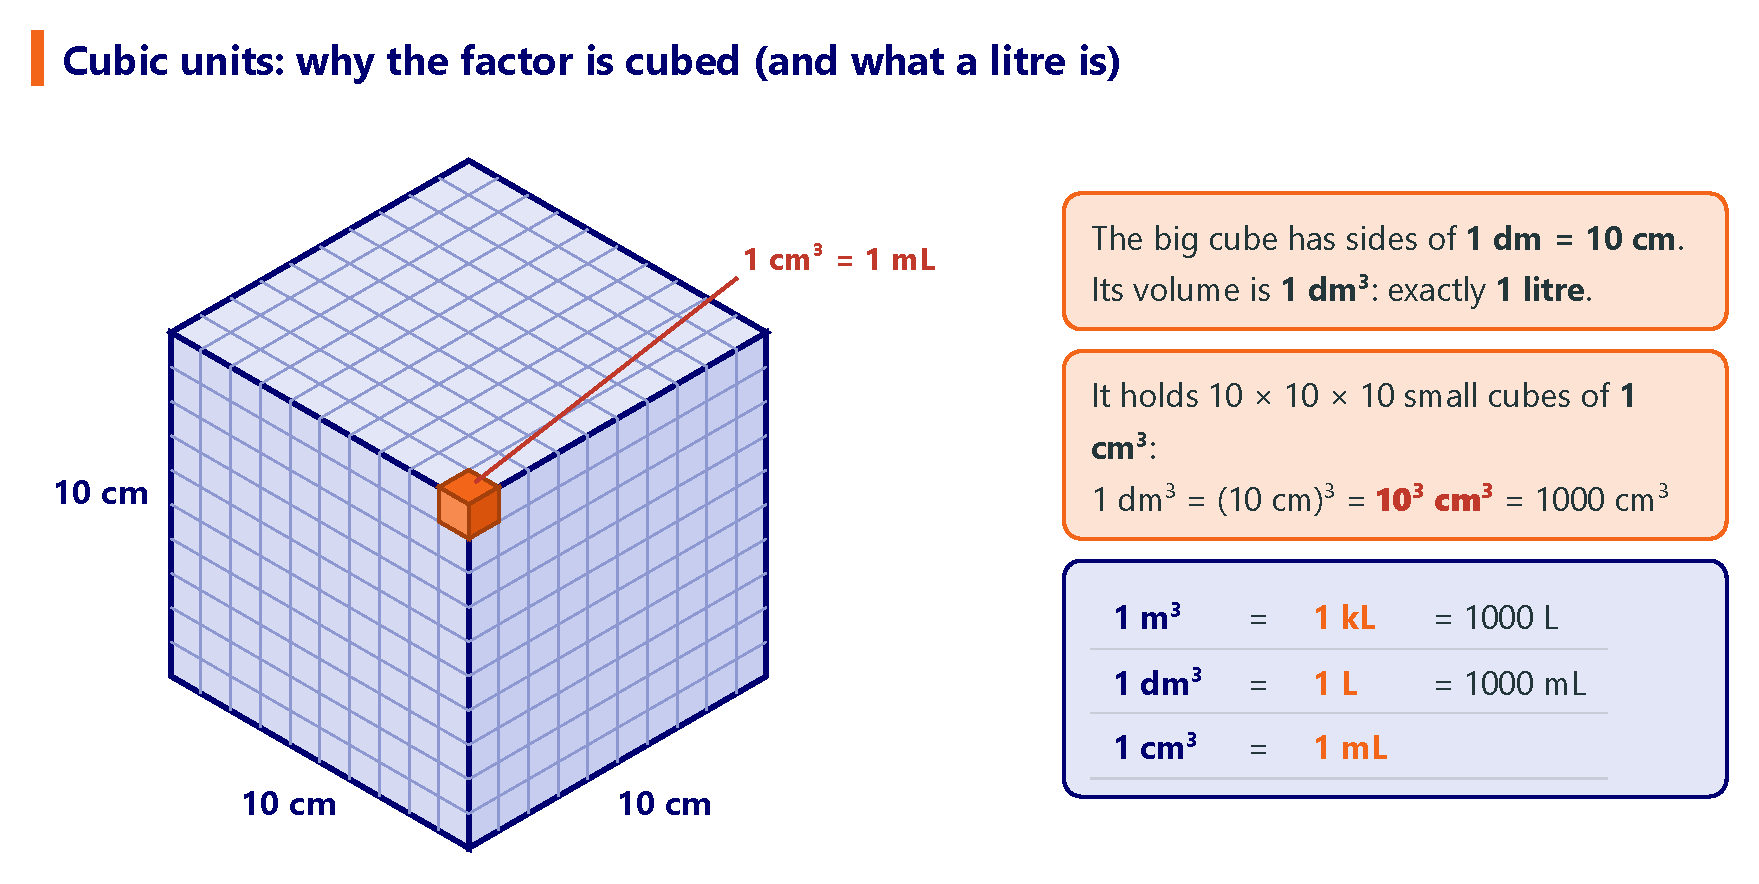
\includegraphics[width=0.9\textwidth]{FigurasSVG/Unit_1_Matter_Measurement/pdf/cube_units.pdf}
    \caption{One cubic decimetre (one litre) contains \(10^{3}\) cubic centimetres (millilitres).}
    \label{fig:u1_cube_units}
\end{figure}

\begin{impt}
    \negsubro{Trick for volume}: we do the same as with surface area, but now we \textbf{raise the factor of length to the power of 3}.
    \begin{equation*}
        \text{Length: } \dfrac{\qty{e2}{\cm}}{\qty{1}{\m}}
        \quad\Longrightarrow\quad
        \text{Volume: } \left(\dfrac{\qty{e2}{\cm}}{\qty{1}{\m}}\right)^{3} = \dfrac{\qty{e6}{\cubic\cm}}{\qty{1}{\cubic\m}}
    \end{equation*}
    Each step on the staircase of volume units is therefore worth \(10^{3} = 1000\).
\end{impt}

\begin{example}
    \textbf{Write \qty{0.5}{\cubic\metre} in \unit{\cubic\mm}.} \\
    Simple change: \(\qty{1}{\m} = \qty{e3}{\mm}\). Cubing the factor:
    \begin{equation*}
        \num{0.5}\,\cancelunit{\cubic\m} \cdot \left(\dfrac{\qty{e3}{\mm}}{1\,\cancelunit{\m}}\right)^{3}
        = \num{0.5}\,\cancelunit{\cubic\m} \cdot \dfrac{\qty{e9}{\cubic\mm}}{1\,\cancelunit{\cubic\m}}
        = \textcolor{red}{\qty{5e8}{\cubic\mm}}
    \end{equation*}
\end{example}

\begin{example}
    \textbf{Write \qty{850}{\cubic\deca\metre} in \unit{\cubic\km}.} \\
    Simple change: \(\qty{1}{\km} = \qty{e2}{\deca\m}\). Cubing the factor:
    \begin{equation*}
        \num{850}\,\cancelunit{\cubic\deca\m} \cdot \left(\dfrac{\qty{1}{\km}}{\num{e2}\,\cancelunit{\deca\m}}\right)^{3}
        = \num{850}\,\cancelunit{\cubic\deca\m} \cdot \dfrac{\qty{1}{\cubic\km}}{\num{e6}\,\cancelunit{\cubic\deca\m}}
        = \qty{850e-6}{\cubic\km} = \textcolor{red}{\qty{8.5e-4}{\cubic\km}}
    \end{equation*}
\end{example}

\begin{exercise}
    Convert these amounts using conversion factors:
    \begin{enumerate}[label=\letraminuscula]
        \item \(\qty{73.357}{\cubic\cm} \to \unit{\cubic\mm}\)
        \item \(\qty{1.0576}{\cubic\deca\metre} \to \unit{\cubic\dm}\)
        \item \(\qty{2500}{\cubic\cm} \to \unit{\cubic\m}\)
    \end{enumerate}
    \begin{solu}
        \begin{enumerate}[label=\alph*)]
            \item \(\num{73.357}\,\unit{\cubic\cm} \cdot \left(\dfrac{\qty{e1}{\mm}}{\qty{1}{\cm}}\right)^{3} = \num{73.357}\,\unit{\cubic\cm} \cdot \dfrac{\qty{e3}{\cubic\mm}}{\qty{1}{\cubic\cm}} = \qty{73357}{\cubic\mm}\)
            \item \(\num{1.0576}\,\unit{\cubic\deca\m} \cdot \left(\dfrac{\qty{e2}{\dm}}{\qty{1}{\deca\m}}\right)^{3} = \num{1.0576}\,\unit{\cubic\deca\m} \cdot \dfrac{\qty{e6}{\cubic\dm}}{\qty{1}{\cubic\deca\m}} = \qty{1.0576e6}{\cubic\dm}\)
            \item \(\num{2500}\,\unit{\cubic\cm} \cdot \left(\dfrac{\qty{1}{\m}}{\qty{e2}{\cm}}\right)^{3} = \num{2500}\,\unit{\cubic\cm} \cdot \dfrac{\qty{1}{\cubic\m}}{\qty{e6}{\cubic\cm}} = \qty{2.5e-3}{\cubic\m}\)
        \end{enumerate}
    \end{solu}
\end{exercise}

\begin{exercise}
    Convert these amounts using conversion factors:
    \begin{enumerate}[label=\letraminuscula]
        \item \(\qty{40}{\cubic\cm} \to \unit{\cubic\dm}\)
        \item \(\qty{e3}{\cubic\km} \to \unit{\cubic\hecto\m}\)
        \item \(\qty{3}{\cubic\deca\m} \to \unit{\cubic\cm}\)
        \item \(\qty{e2}{\cubic\cm} \to \unit{\cubic\dm}\)
        \item \(\qty{7}{\cubic\mm} \to \unit{\cubic\deca\m}\)
        \item \(\qty{2e-2}{\cubic\m} \to \unit{\cubic\mm}\)
        \item \(\qty{5e2}{\cubic\km} \to \unit{\cubic\hecto\m}\)
        \item \(\qty{4.23}{\cubic\deca\m} \to \unit{\cubic\cm}\)
        \item \(\qty{48}{\cubic\cm} \to \unit{\cubic\dm}\)
    \end{enumerate}
    \begin{solu}
        \begin{enumerate}[label=\alph*)]
            \item \(\num{40}\,\unit{\cubic\cm} \cdot \left(\dfrac{\qty{1}{\dm}}{\qty{e1}{\cm}}\right)^{3} = \num{40}\,\unit{\cubic\cm} \cdot \dfrac{\qty{1}{\cubic\dm}}{\qty{e3}{\cubic\cm}} = \qty{4e-2}{\cubic\dm} = \qty{0.04}{\cubic\dm}\)
            \item \(\num{e3}\,\unit{\cubic\km} \cdot \left(\dfrac{\qty{e1}{\hecto\m}}{\qty{1}{\km}}\right)^{3} = \num{e3}\,\unit{\cubic\km} \cdot \dfrac{\qty{e3}{\cubic\hecto\m}}{\qty{1}{\cubic\km}} = \qty{e6}{\cubic\hecto\m}\)
            \item \(\num{3}\,\unit{\cubic\deca\m} \cdot \left(\dfrac{\qty{e3}{\cm}}{\qty{1}{\deca\m}}\right)^{3} = \num{3}\,\unit{\cubic\deca\m} \cdot \dfrac{\qty{e9}{\cubic\cm}}{\qty{1}{\cubic\deca\m}} = \qty{3e9}{\cubic\cm}\)
            \item \(\num{e2}\,\unit{\cubic\cm} \cdot \left(\dfrac{\qty{1}{\dm}}{\qty{e1}{\cm}}\right)^{3} = \num{e2}\,\unit{\cubic\cm} \cdot \dfrac{\qty{1}{\cubic\dm}}{\qty{e3}{\cubic\cm}} = \qty{e-1}{\cubic\dm} = \qty{0.1}{\cubic\dm}\)
            \item \(\num{7}\,\unit{\cubic\mm} \cdot \left(\dfrac{\qty{1}{\deca\m}}{\qty{e4}{\mm}}\right)^{3} = \num{7}\,\unit{\cubic\mm} \cdot \dfrac{\qty{1}{\cubic\deca\m}}{\qty{e12}{\cubic\mm}} = \qty{7e-12}{\cubic\deca\m}\)
            \item \(\num{2e-2}\,\unit{\cubic\m} \cdot \left(\dfrac{\qty{e3}{\mm}}{\qty{1}{\m}}\right)^{3} = \num{2e-2}\,\unit{\cubic\m} \cdot \dfrac{\qty{e9}{\cubic\mm}}{\qty{1}{\cubic\m}} = \qty{2e7}{\cubic\mm}\)
            \item \(\num{5e2}\,\unit{\cubic\km} \cdot \left(\dfrac{\qty{e1}{\hecto\m}}{\qty{1}{\km}}\right)^{3} = \num{5e2}\,\unit{\cubic\km} \cdot \dfrac{\qty{e3}{\cubic\hecto\m}}{\qty{1}{\cubic\km}} = \qty{5e5}{\cubic\hecto\m}\)
            \item \(\num{4.23}\,\unit{\cubic\deca\m} \cdot \left(\dfrac{\qty{e3}{\cm}}{\qty{1}{\deca\m}}\right)^{3} = \num{4.23}\,\unit{\cubic\deca\m} \cdot \dfrac{\qty{e9}{\cubic\cm}}{\qty{1}{\cubic\deca\m}} = \qty{4.23e9}{\cubic\cm}\)
            \item \(\num{48}\,\unit{\cubic\cm} \cdot \left(\dfrac{\qty{1}{\dm}}{\qty{e1}{\cm}}\right)^{3} = \num{48}\,\unit{\cubic\cm} \cdot \dfrac{\qty{1}{\cubic\dm}}{\qty{e3}{\cubic\cm}} = \qty{4.8e-2}{\cubic\dm} = \qty{0.048}{\cubic\dm}\)
        \end{enumerate}
    \end{solu}
\end{exercise}

%------------------------------------------------

\subsubsection{Volume and capacity: cubic units and litres}

We use \textbf{volume} for the space occupied by a body and \textbf{capacity} for what a container can hold, but they are the same quantity, so their units are related. The three key equivalences are:

\begin{table}[H]
    \centering
    \renewcommand{\arraystretch}{1.4}
    \begin{tabular}{ccc}
        \toprule
        \textbf{Volume} & & \textbf{Capacity} \\
        \midrule
        \qty{1}{\cubic\m} & = & \qty{1}{\kilo\litre} \\
        \qty{1}{\cubic\dm} & = & \qty{1}{\litre} \\
        \qty{1}{\cubic\cm} & = & \qty{1}{\mL} \\
        \bottomrule
    \end{tabular}
    \caption{Equivalences between volume and capacity units.}
    \label{tab:u1_volume_capacity}
\end{table}

\begin{impt}
    To change between cubic units and litres:
    \begin{enumerate}[label=\numberballmDarkTeal]
        \item Use the conversion factors of volume (cubed) or of capacity (simple) to reach one of the three ``partner'' units: \unit{\cubic\m}--\unit{\kilo\litre}, \unit{\cubic\dm}--\unit{\litre} or \unit{\cubic\cm}--\unit{\mL}.
        \item Jump from volume to capacity (or the other way round) with a factor such as \(\dfrac{\qty{1}{\litre}}{\qty{1}{\cubic\dm}}\), which is worth 1.
    \end{enumerate}
\end{impt}

\begin{example}
    \textbf{Write \qty{2.5}{\cubic\m} in litres.}
    \begin{equation*}
        \num{2.5}\,\cancelunit{\cubic\m} \cdot \dfrac{\qty{1}{\kilo\litre}}{1\,\cancelunit{\cubic\m}} \cdot \dfrac{\qty{e3}{\litre}}{1\,\cancelunit{\kilo\litre}} = \textcolor{red}{\qty{2.5e3}{\litre}} = \qty{2500}{\litre}
    \end{equation*}
\end{example}

\begin{example}
    \textbf{A soft drink can contains \qty{33}{\centi\litre}. Write it in \unit{\cubic\cm}.}
    \begin{equation*}
        \num{33}\,\cancelunit{\centi\litre} \cdot \dfrac{\num{e1}\,\cancelunit{\mL}}{1\,\cancelunit{\centi\litre}} \cdot \dfrac{\qty{1}{\cubic\cm}}{1\,\cancelunit{\mL}} = \textcolor{red}{\qty{330}{\cubic\cm}}
    \end{equation*}
\end{example}

\begin{example}
    \textbf{Write \qty{750}{\mL} in \unit{\cubic\m}.}
    \begin{equation*}
        \num{750}\,\cancelunit{\mL} \cdot \dfrac{1\,\cancelunit{\cubic\cm}}{1\,\cancelunit{\mL}} \cdot \left(\dfrac{\qty{1}{\m}}{\num{e2}\,\cancelunit{\cm}}\right)^{3}
        = \num{750}\,\cancelunit{\cubic\cm} \cdot \dfrac{\qty{1}{\cubic\m}}{\num{e6}\,\cancelunit{\cubic\cm}} = \textcolor{red}{\qty{7.5e-4}{\cubic\m}}
    \end{equation*}
\end{example}

\begin{exercise}
    An Olympic-size swimming pool contains 2.5 million litres of water (\qty{2.5e6}{\litre}). Write it in \unit{\cubic\metre}.
    \begin{solu}
        \(\num{2.5e6}\,\unit{\litre} \cdot \dfrac{\qty{1}{\cubic\dm}}{\qty{1}{\litre}} \cdot \left(\dfrac{\qty{1}{\m}}{\qty{e1}{\dm}}\right)^{3} = \num{2.5e6}\,\unit{\cubic\dm} \cdot \dfrac{\qty{1}{\cubic\m}}{\qty{e3}{\cubic\dm}} = \qty{2.5e3}{\cubic\m} = \qty{2500}{\cubic\m}\).
    \end{solu}
\end{exercise}

\begin{exercise}
    Convert: \textbf{a)} \qty{1.5}{\litre} \(\to\) \unit{\cubic\cm}; \textbf{b)} \qty{40}{\cubic\cm} \(\to\) \unit{\centi\litre}; \textbf{c)} \qty{0.2}{\cubic\m} \(\to\) \unit{\litre}; \textbf{d)} \qty{5}{\mL} \(\to\) \unit{\cubic\dm}.
    \begin{solu}
        a) \(\num{1.5}\,\unit{\litre} \cdot \dfrac{\qty{e3}{\mL}}{\qty{1}{\litre}} \cdot \dfrac{\qty{1}{\cubic\cm}}{\qty{1}{\mL}} = \qty{1500}{\cubic\cm}\) \\
        b) \(\num{40}\,\unit{\cubic\cm} \cdot \dfrac{\qty{1}{\mL}}{\qty{1}{\cubic\cm}} \cdot \dfrac{\qty{1}{\centi\litre}}{\qty{e1}{\mL}} = \qty{4}{\centi\litre}\) \\
        c) \(\num{0.2}\,\unit{\cubic\m} \cdot \dfrac{\qty{1}{\kilo\litre}}{\qty{1}{\cubic\m}} \cdot \dfrac{\qty{e3}{\litre}}{\qty{1}{\kilo\litre}} = \qty{200}{\litre}\) \\
        d) \(\num{5}\,\unit{\mL} \cdot \dfrac{\qty{1}{\litre}}{\qty{e3}{\mL}} \cdot \dfrac{\qty{1}{\cubic\dm}}{\qty{1}{\litre}} = \qty{5e-3}{\cubic\dm}\)
    \end{solu}
\end{exercise}

\begin{exercise}
    A fish tank is a rectangular prism \qty{50}{\cm} long, \qty{30}{\cm} wide and \qty{40}{\cm} high.
    \begin{enumerate}[label=\letraminuscula]
        \item Calculate its volume in \unit{\cubic\cm}.
        \item How many litres of water are needed to fill it completely?
    \end{enumerate}
    \begin{solu}
        \begin{enumerate}[label=\alph*)]
            \item \(V = \qty{50}{\cm} \cdot \qty{30}{\cm} \cdot \qty{40}{\cm} = \qty{60000}{\cubic\cm} = \qty{6e4}{\cubic\cm}\).
            \item \(\num{6e4}\,\unit{\cubic\cm} \cdot \dfrac{\qty{1}{\mL}}{\qty{1}{\cubic\cm}} \cdot \dfrac{\qty{1}{\litre}}{\qty{e3}{\mL}} = \qty{60}{\litre}\).
        \end{enumerate}
    \end{solu}
\end{exercise}

\begin{exercise}
    Convert these amounts using conversion factors:
    \begin{enumerate}[label=\letraminuscula]
        \item \(\qty{0.02}{\cubic\deca\m} \to \unit{\mL}\)
        \item \(\qty{100}{\mL} \to \unit{\cubic\m}\)
        \item \(\qty{300}{\litre} \to \unit{\cubic\deca\m}\)
    \end{enumerate}
    \begin{solu}
        \begin{enumerate}[label=\alph*)]
            \item \(\num{0.02}\,\unit{\cubic\deca\m} \cdot \left(\dfrac{\qty{e3}{\cm}}{\qty{1}{\deca\m}}\right)^{3} \cdot \dfrac{\qty{1}{\mL}}{\qty{1}{\cubic\cm}} = \num{0.02}\,\unit{\cubic\deca\m} \cdot \dfrac{\qty{e9}{\cubic\cm}}{\qty{1}{\cubic\deca\m}} \cdot \dfrac{\qty{1}{\mL}}{\qty{1}{\cubic\cm}} = \qty{2e7}{\mL}\)
            \item \(\num{100}\,\unit{\mL} \cdot \dfrac{\qty{1}{\cubic\cm}}{\qty{1}{\mL}} \cdot \left(\dfrac{\qty{1}{\m}}{\qty{e2}{\cm}}\right)^{3} = \num{100}\,\unit{\cubic\cm} \cdot \dfrac{\qty{1}{\cubic\m}}{\qty{e6}{\cubic\cm}} = \qty{e-4}{\cubic\m}\)
            \item \(\num{300}\,\unit{\litre} \cdot \dfrac{\qty{1}{\cubic\dm}}{\qty{1}{\litre}} \cdot \left(\dfrac{\qty{1}{\deca\m}}{\qty{e2}{\dm}}\right)^{3} = \num{300}\,\unit{\cubic\dm} \cdot \dfrac{\qty{1}{\cubic\deca\m}}{\qty{e6}{\cubic\dm}} = \qty{3e-4}{\cubic\deca\m}\)
        \end{enumerate}
    \end{solu}
\end{exercise}

%------------------------------------------------

\subsubsection{Time}

In the SI, time is measured in \textbf{seconds} (\unit{\s}). For longer times we use minutes, hours, days, weeks and years. \textbf{Be careful}: these units are \textbf{not} related by powers of 10, so we cannot use the prefix staircase. We must use their real equivalences.

\begin{figure}[H]
    \centering
    % [FIGURA ORIGINAL] \includegraphics[width=\textwidth]{Unit_1/time_chain}
    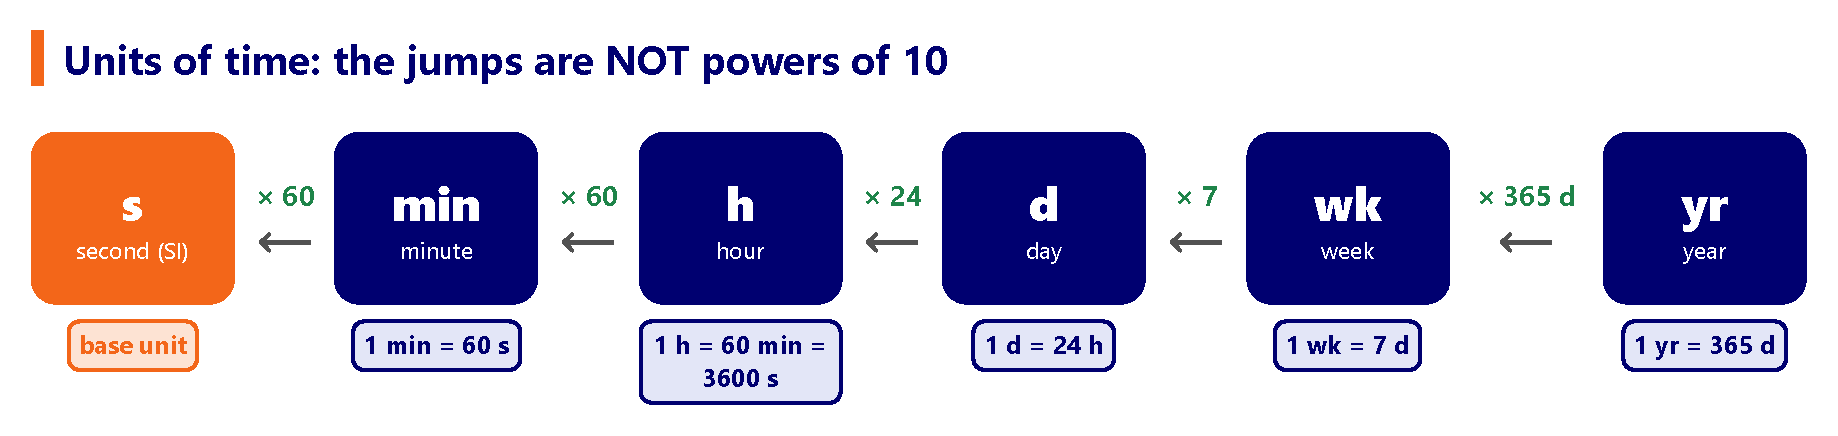
\includegraphics[width=\textwidth]{FigurasSVG/Unit_1_Matter_Measurement/pdf/time_chain.pdf}
    \caption{The chain of time units.}
    \label{fig:u1_time_chain}
\end{figure}

\begin{table}[H]
    \centering
    \renewcommand{\arraystretch}{2.4}
    \begin{tabular}{ll}
        \toprule
        \textbf{Equivalence} & \textbf{Conversion factors} \\
        \midrule
        \(\qty{1}{\minute} = \qty{60}{\s}\) & \(\dfrac{\qty{60}{\s}}{\qty{1}{\minute}}\) or \(\dfrac{\qty{1}{\minute}}{\qty{60}{\s}}\) \\
        \(\qty{1}{\hour} = \qty{60}{\minute} = \qty{3600}{\s}\) & \(\dfrac{\qty{3600}{\s}}{\qty{1}{\hour}}\) or \(\dfrac{\qty{1}{\hour}}{\qty{3600}{\s}}\) \\
        \(\qty{1}{\day} = \qty{24}{\hour}\) & \(\dfrac{\qty{24}{\hour}}{\qty{1}{\day}}\) or \(\dfrac{\qty{1}{\day}}{\qty{24}{\hour}}\) \\
        \(\qty{1}{week} = \qty{7}{\day}\) & \(\dfrac{\qty{7}{\day}}{\qty{1}{week}}\) or \(\dfrac{\qty{1}{week}}{\qty{7}{\day}}\) \\
        \(\qty{1}{year} = \qty{365}{\day}\) & \(\dfrac{\qty{365}{\day}}{\qty{1}{year}}\) or \(\dfrac{\qty{1}{year}}{\qty{365}{\day}}\) \\
        \bottomrule
    \end{tabular}
    \caption{Time equivalences and their conversion factors.}
    \label{tab:u1_time}
\end{table}

\begin{example}
    \textbf{Write \qty{5000}{\s} in hours.}
    \begin{equation*}
        \num{5000}\,\cancelunit{\s} \cdot \dfrac{\qty{1}{\hour}}{\num{3600}\,\cancelunit{\s}} = \dfrac{5000}{3600}\,\unit{\hour} = \textcolor{red}{\qty{1.39}{\hour}}
    \end{equation*}
\end{example}

\begin{example}
    \textbf{How many seconds are there in 2 weeks?} There is no direct equivalence, so we link several factors:
    \begin{equation*}
        \num{2}\,\cancelunit{week} \cdot \dfrac{\num{7}\,\cancelunit{\day}}{1\,\cancelunit{week}} \cdot \dfrac{\num{24}\,\cancelunit{\hour}}{1\,\cancelunit{\day}} \cdot \dfrac{\qty{3600}{\s}}{1\,\cancelunit{\hour}} = \qty{1209600}{\s} \approx \textcolor{red}{\qty{1.21e6}{\s}}
    \end{equation*}
\end{example}

\begin{exercise}
    A film is \qty{135}{\minute} long. How many hours does it last? A song lasts \qty{4.5}{\minute}. How many seconds does it last?
    \begin{solu}
        \(\num{135}\,\unit{\minute} \cdot \dfrac{\qty{1}{\hour}}{\qty{60}{\minute}} = \qty{2.25}{\hour}\). \\
        \(\num{4.5}\,\unit{\minute} \cdot \dfrac{\qty{60}{\s}}{\qty{1}{\minute}} = \qty{270}{\s}\).
    \end{solu}
\end{exercise}

\begin{exercise}
    Convert: \textbf{a)} \qty{3}{\day} \(\to\) \unit{\minute}; \textbf{b)} \qty{90}{\minute} \(\to\) \unit{\hour}; \textbf{c)} \qty{86400}{\s} \(\to\) \unit{\day}; \textbf{d)} \qty{1}{year} \(\to\) weeks.
    \begin{solu}
        a) \(\num{3}\,\unit{\day} \cdot \dfrac{\qty{24}{\hour}}{\qty{1}{\day}} \cdot \dfrac{\qty{60}{\minute}}{\qty{1}{\hour}} = \qty{4320}{\minute}\) \\
        b) \(\num{90}\,\unit{\minute} \cdot \dfrac{\qty{1}{\hour}}{\qty{60}{\minute}} = \qty{1.5}{\hour}\) \\
        c) \(\num{86400}\,\unit{\s} \cdot \dfrac{\qty{1}{\hour}}{\qty{3600}{\s}} \cdot \dfrac{\qty{1}{\day}}{\qty{24}{\hour}} = \qty{1}{\day}\) \\
        d) \(\num{1}\,\unit{year} \cdot \dfrac{\qty{365}{\day}}{\qty{1}{year}} \cdot \dfrac{\qty{1}{week}}{\qty{7}{\day}} \approx \qty{52.1}{weeks}\)
    \end{solu}
\end{exercise}

\begin{exercise}
    You are 12 years old. How many seconds have you lived, approximately? Give the result as a power of 10.
    \begin{solu}
        \(\num{12}\,\unit{year} \cdot \dfrac{\qty{365}{\day}}{\qty{1}{year}} \cdot \dfrac{\qty{24}{\hour}}{\qty{1}{\day}} \cdot \dfrac{\qty{3600}{\s}}{\qty{1}{\hour}} = \qty{378432000}{\s} \approx \qty{3.78e8}{\s}\).
    \end{solu}
\end{exercise}

\begin{exercise}
    Convert these times using conversion factors:
    \begin{enumerate}[label=\letraminuscula]
        \item \(\qty{340}{\minute} \to \unit{\s}\)
        \item \(\qty{6.2}{\hour} \to \unit{\minute}\)
        \item \(\qty{10}{\hour} \to \unit{\s}\)
        \item \(\qty{28}{weeks} \to \unit{\minute}\)
        \item \(\qty{22}{weeks} \to \unit{\hour}\)
    \end{enumerate}
    \begin{solu}
        \begin{enumerate}[label=\alph*)]
            \item \(\num{340}\,\unit{\minute} \cdot \dfrac{\qty{60}{\s}}{\qty{1}{\minute}} = \qty{20400}{\s} \approx \qty{2.04e4}{\s}\)
            \item \(\num{6.2}\,\unit{\hour} \cdot \dfrac{\qty{60}{\minute}}{\qty{1}{\hour}} = \qty{372}{\minute}\)
            \item \(\num{10}\,\unit{\hour} \cdot \dfrac{\qty{3600}{\s}}{\qty{1}{\hour}} = \qty{36000}{\s} = \qty{3.6e4}{\s}\)
            \item \(\num{28}\,\unit{weeks} \cdot \dfrac{\qty{7}{\day}}{\qty{1}{week}} \cdot \dfrac{\qty{24}{\hour}}{\qty{1}{\day}} \cdot \dfrac{\qty{60}{\minute}}{\qty{1}{\hour}} = \qty{282240}{\minute} \approx \qty{2.82e5}{\minute}\)
            \item \(\num{22}\,\unit{weeks} \cdot \dfrac{\qty{7}{\day}}{\qty{1}{week}} \cdot \dfrac{\qty{24}{\hour}}{\qty{1}{\day}} = \qty{3696}{\hour}\)
        \end{enumerate}
    \end{solu}
\end{exercise}

%------------------------------------------------

\subsubsection{Speed}

Speed is a derived quantity (length \(\div\) time), so its unit has \textbf{two} parts. To change it, we use \textbf{two} conversion factors: one for the length (numerator) and one for the time (denominator).

\begin{impt}
    \negsubro{Units with more than one quantity: one unit at a time, in order}

    When a unit is made of two quantities (\unit{\km\per\hour}, \unit{\g\per\mL}\ldots), we do \textbf{not} try to change both at once. We go \textbf{in order}:
    \begin{enumerate}[label=\numberballmDarkTeal]
        \item First we change \textbf{one} of the units (for example, the length: \unit{\km} \(\to\) \unit{\m}) with its own conversion factor.
        \item Then we change the \textbf{other} unit (the time: \unit{\hour} \(\to\) \unit{\s}) with a second conversion factor.
        \item Finally we cancel the units and calculate.
        \item Steps 1 and 2 \textbf{can and should} be done \textbf{all in one line}: we write the first conversion factor and, right after it, the second one, without stopping to calculate the intermediate result. We cancel all the units at the end and do only one calculation.
    \end{enumerate}
    Step by step for \qty{90}{\km\per\hour}:
    \begin{equation*}
        \underbrace{\num{90}\,\dfrac{\cancelunit{\km}}{\unit{\hour}} \cdot \dfrac{\qty{e3}{\m}}{1\,\cancelunit{\km}} = \qty{90000}{\m\per\hour}}_{\text{1st: the length}}
        \quad\Longrightarrow\quad
        \underbrace{\num{90000}\,\dfrac{\unit{\m}}{\cancelunit{\hour}} \cdot \dfrac{1\,\cancelunit{\hour}}{\qty{3600}{\s}} = \qty{25}{\m\per\s}}_{\text{2nd: the time}}
    \end{equation*}
    All in one line (this is how we must do it):
    \begin{equation*}
        \num{90}\,\dfrac{\cancelunit{\km}}{\cancelunit{\hour}} \cdot \underbrace{\dfrac{\qty{e3}{\m}}{1\,\cancelunit{\km}}}_{\text{1st: length}} \cdot \underbrace{\dfrac{1\,\cancelunit{\hour}}{\qty{3600}{\s}}}_{\text{2nd: time}} = \dfrac{\num{90e3}}{3600}\,\unit{\m\per\s} = \qty{25}{\m\per\s}
    \end{equation*}
\end{impt}

\begin{figure}[H]
    \centering
    % [FIGURA ORIGINAL] \includegraphics[width=0.85\textwidth]{Unit_1/speed_shortcut}
    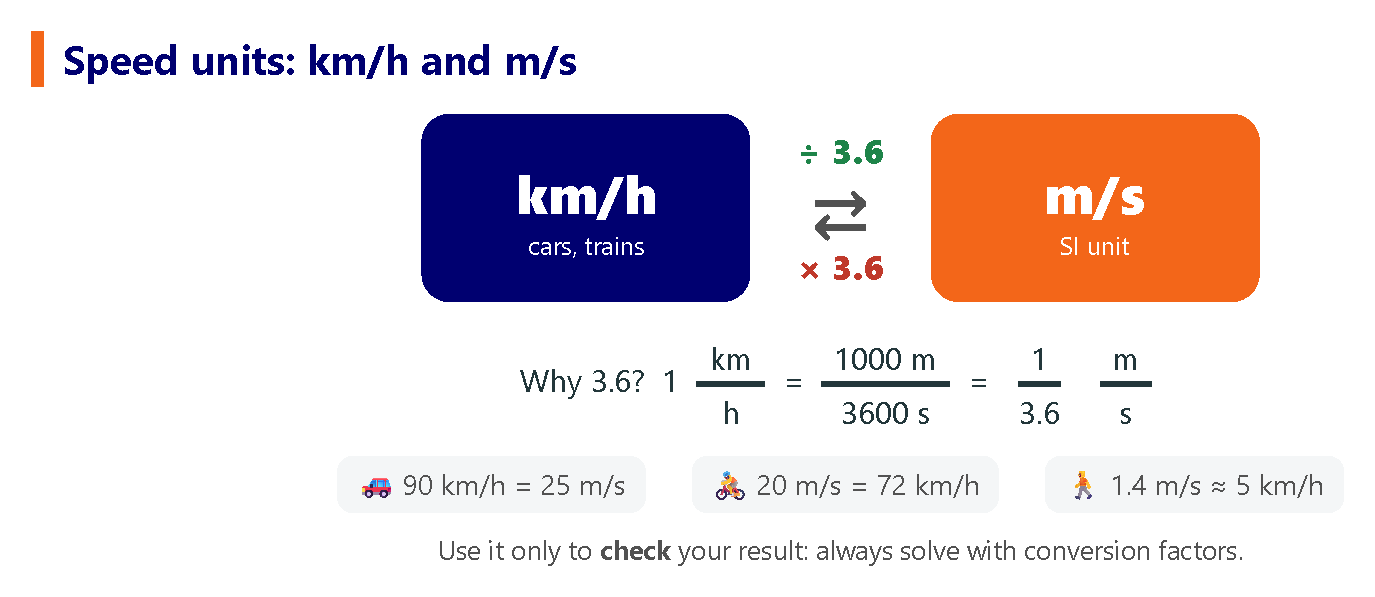
\includegraphics[width=0.85\textwidth]{FigurasSVG/Unit_1_Matter_Measurement/pdf/speed_shortcut.pdf}
    \caption{The two most common units of speed and a quick way to check your result.}
    \label{fig:u1_speed_shortcut}
\end{figure}

\begin{example}
    \textbf{A car travels at \qty{90}{\km\per\hour}. Write this speed in \unit{\m\per\s}.}
    \begin{equation*}
        \num{90}\,\dfrac{\cancelunit{\km}}{\cancelunit{\hour}} \cdot \dfrac{\qty{e3}{\m}}{1\,\cancelunit{\km}} \cdot \dfrac{1\,\cancelunit{\hour}}{\qty{3600}{\s}} = \dfrac{\num{90e3}}{3600}\,\unit{\m\per\s} = \textcolor{red}{\qty{25}{\m\per\s}}
    \end{equation*}
\end{example}

\begin{example}
    \textbf{A cyclist rides at \qty{20}{\m\per\s}. Write this speed in \unit{\km\per\hour}.}
    \begin{equation*}
        \num{20}\,\dfrac{\cancelunit{\m}}{\cancelunit{\s}} \cdot \dfrac{\qty{1}{\km}}{\num{e3}\,\cancelunit{\m}} \cdot \dfrac{\num{3600}\,\cancelunit{\s}}{\qty{1}{\hour}} = \textcolor{red}{\qty{72}{\km\per\hour}}
    \end{equation*}
\end{example}

\begin{marker}
    \textbf{Dividing or multiplying by 3.6 is only a help.} The ``trick'' in the figure (\(\div\,3.6\) to go from \unit{\km\per\hour} to \unit{\m\per\s}, and \(\times\,3.6\) to go back) is only useful to \textbf{check} your result, and it \textbf{only works for that change}: \unit{\km\per\hour} \(\leftrightarrow\) \unit{\m\per\s}. For any other unit of speed (\unit{\cm\per\s}, \unit{\m\per\minute}, \unit{\km\per\minute}\ldots) it gives a wrong answer. The right way, which \textbf{always} works, is to use \textbf{conversion factors}.
\end{marker}

\begin{example}
    \textbf{A tortoise walks at \qty{12}{\m\per\minute}. Write this speed in \unit{\m\per\s}.} Only the time changes, so we need just one factor:
    \begin{equation*}
        \num{12}\,\dfrac{\unit{\m}}{\cancelunit{\minute}} \cdot \dfrac{1\,\cancelunit{\minute}}{\qty{60}{\s}} = \textcolor{red}{\qty{0.2}{\m\per\s}}
    \end{equation*}
\end{example}

\begin{example}
    \textbf{A toy car moves at \qty{45}{\cm\per\s}. Write this speed in \unit{\km\per\hour}.} First the length, then the time:
    \begin{equation*}
        \num{45}\,\dfrac{\cancelunit{\cm}}{\cancelunit{\s}} \cdot \dfrac{\qty{1}{\km}}{\num{e5}\,\cancelunit{\cm}} \cdot \dfrac{\num{3600}\,\cancelunit{\s}}{\qty{1}{\hour}} = \dfrac{\num{45} \cdot \num{3600}}{\num{e5}}\,\unit{\km\per\hour} = \textcolor{red}{\qty{1.62}{\km\per\hour}}
    \end{equation*}
\end{example}

\begin{example}
    \textbf{A plane flies at \qty{15}{\km\per\minute}. Write this speed in \unit{\m\per\s}.} First the length, then the time:
    \begin{equation*}
        \num{15}\,\dfrac{\cancelunit{\km}}{\cancelunit{\minute}} \cdot \dfrac{\qty{e3}{\m}}{1\,\cancelunit{\km}} \cdot \dfrac{1\,\cancelunit{\minute}}{\qty{60}{\s}} = \dfrac{\num{15e3}}{60}\,\unit{\m\per\s} = \textcolor{red}{\qty{250}{\m\per\s}}
    \end{equation*}
\end{example}

\begin{example}
    \textbf{A snail moves at \qty{0.5}{\mm\per\s}. Write this speed in \unit{\m\per\hour}.} First the length, then the time:
    \begin{equation*}
        \num{0.5}\,\dfrac{\cancelunit{\mm}}{\cancelunit{\s}} \cdot \dfrac{\qty{1}{\m}}{\num{e3}\,\cancelunit{\mm}} \cdot \dfrac{\num{3600}\,\cancelunit{\s}}{\qty{1}{\hour}} = \textcolor{red}{\qty{1.8}{\m\per\hour}}
    \end{equation*}
\end{example}

\begin{exercise}
    An athlete runs \qty{100}{\metre} in \qty{11.5}{\s}. Calculate her average speed in \unit{\m\per\s} and in \unit{\km\per\hour}.
    \begin{solu}
        \(v = \dfrac{\qty{100}{\m}}{\qty{11.5}{\s}} \approx \qty{8.70}{\m\per\s}\). \\
        \(\num{8.70}\,\dfrac{\unit{\m}}{\unit{\s}} \cdot \dfrac{\qty{1}{\km}}{\qty{e3}{\m}} \cdot \dfrac{\qty{3600}{\s}}{\qty{1}{\hour}} \approx \qty{31.3}{\km\per\hour}\).
    \end{solu}
\end{exercise}

\begin{exercise}
    Convert these speeds:
    \begin{enumerate}[label=\letraminuscula]
        \item The speed limit on a motorway, \qty{120}{\km\per\hour}, to \unit{\m\per\s}.
        \item The speed of light, \qty{3e5}{\km\per\s}, to \unit{\m\per\s}.
        \item A snail moving at \qty{1.3}{\cm\per\s}, to \unit{\km\per\hour}.
    \end{enumerate}
    \begin{solu}
        \begin{enumerate}[label=\alph*)]
            \item \(\num{120}\,\dfrac{\unit{\km}}{\unit{\hour}} \cdot \dfrac{\qty{e3}{\m}}{\qty{1}{\km}} \cdot \dfrac{\qty{1}{\hour}}{\qty{3600}{\s}} \approx \qty{33.3}{\m\per\s}\)
            \item \(\num{3e5}\,\dfrac{\unit{\km}}{\unit{\s}} \cdot \dfrac{\qty{e3}{\m}}{\qty{1}{\km}} = \qty{3e8}{\m\per\s}\)
            \item \(\num{1.3}\,\dfrac{\unit{\cm}}{\unit{\s}} \cdot \dfrac{\qty{1}{\km}}{\qty{e5}{\cm}} \cdot \dfrac{\qty{3600}{\s}}{\qty{1}{\hour}} \approx \qty{0.047}{\km\per\hour}\)
        \end{enumerate}
    \end{solu}
\end{exercise}

\begin{exercise}
    Convert: \textbf{a)} \qty{36}{\m\per\s} \(\to\) \unit{\km\per\hour}; \textbf{b)} \qty{100}{\km\per\hour} \(\to\) \unit{\m\per\s}.
    \begin{solu}
        a) \(\num{36}\,\dfrac{\unit{\m}}{\unit{\s}} \cdot \dfrac{\qty{1}{\km}}{\qty{e3}{\m}} \cdot \dfrac{\qty{3600}{\s}}{\qty{1}{\hour}} = \qty{129.6}{\km\per\hour}\) \\
        b) \(\num{100}\,\dfrac{\unit{\km}}{\unit{\hour}} \cdot \dfrac{\qty{e3}{\m}}{\qty{1}{\km}} \cdot \dfrac{\qty{1}{\hour}}{\qty{3600}{\s}} \approx \qty{27.8}{\m\per\s}\)
    \end{solu}
\end{exercise}

%------------------------------------------------

\subsubsection{Density}

Density also combines two quantities (mass and volume), so we usually need \textbf{two} conversion factors, one for each unit. Remember to go \textbf{in order}: first we change the unit of mass and then the unit of volume, always \textbf{one at a time}.

\begin{example}
    \textbf{Write the density of ketchup, \qty{1.16}{\g\per\mL}, in \unit{\kg\per\cubic\metre}.}
    \begin{enumerate}[label=\numberballmDarkTeal]
        \item Equivalences: \(\qty{1}{\kg} = \qty{e3}{\g}\) and \(\qty{1}{\cubic\metre} = \qty{1}{\kilo\litre} = \qty{e6}{\mL}\).
        \item Conversion factors:
        \(
            \num{1.16}\,\dfrac{\cancelunit{\g}}{\cancelunit{\mL}} \cdot \dfrac{\qty{1}{\kg}}{\num{e3}\,\cancelunit{\g}} \cdot \dfrac{\num{e6}\,\cancelunit{\mL}}{\qty{1}{\cubic\m}}
        \)
        \item Result: \(\textcolor{red}{\qty{1.16e3}{\kg\per\cubic\metre}} = \qty{1160}{\kg\per\cubic\m}\).
    \end{enumerate}
\end{example}

\begin{exercise}
    Mercury is a liquid metal. \qty{1}{\litre} of mercury has a mass of \qty{13.59}{\kg}. Write its density in \unit{\kg\per\cubic\metre}.
    \begin{solu}
        \(d = \dfrac{\qty{13.59}{\kg}}{\qty{1}{\litre}} \cdot \dfrac{\qty{e3}{\litre}}{\qty{1}{\cubic\m}} = \qty{1.359e4}{\kg\per\cubic\metre}\).
    \end{solu}
\end{exercise}

\begin{exercise}
    The air we breathe has a density of approximately \qty{1.29}{\kg\per\cubic\metre}. Write it in \unit{\g\per\litre}.
    \begin{solu}
        \(d = \num{1.29}\,\dfrac{\unit{\kg}}{\unit{\cubic\m}} \cdot \dfrac{\qty{e3}{\g}}{\qty{1}{\kg}} \cdot \dfrac{\qty{1}{\cubic\m}}{\qty{e3}{\litre}} = \qty{1.29}{\g\per\litre}\).
    \end{solu}
\end{exercise}

\begin{exercise}
    A certain type of wood has a density of \qty{750}{\kg\per\cubic\metre}. Write it in \unit{\g\per\mL}, and decide whether this wood floats in water.
    \begin{solu}
        \(\num{750}\,\dfrac{\unit{\kg}}{\unit{\cubic\m}} \cdot \dfrac{\qty{e3}{\g}}{\qty{1}{\kg}} \cdot \dfrac{\qty{1}{\cubic\m}}{\qty{e6}{\mL}} = \qty{0.75}{\g\per\mL}\). \\
        Since \(\qty{0.75}{\g\per\mL} < \qty{1.00}{\g\per\mL}\), this wood \textbf{floats} in water.
    \end{solu}
\end{exercise}

\begin{exercise}
    Convert these densities using conversion factors:
    \begin{enumerate}[label=\letraminuscula]
        \item \(\qty{1.05}{\kg\per\cubic\cm} \to \unit{\hecto\gram\per\cubic\mm}\)
        \item \(\qty{0.25}{\g\per\mL} \to \unit{\kg\per\cubic\m}\)
        \item \(\qty{0.05}{\kg\per\cubic\cm} \to \unit{\g\per\mL}\)
    \end{enumerate}
    \begin{solu}
        \begin{enumerate}[label=\alph*)]
            \item \(\num{1.05}\,\dfrac{\unit{\kg}}{\unit{\cubic\cm}} \cdot \dfrac{\qty{e1}{\hecto\gram}}{\qty{1}{\kg}} \cdot \left(\dfrac{\qty{1}{\cm}}{\qty{e1}{\mm}}\right)^{3} = \num{1.05}\,\dfrac{\unit{\kg}}{\unit{\cubic\cm}} \cdot \dfrac{\qty{e1}{\hecto\gram}}{\qty{1}{\kg}} \cdot \dfrac{\qty{1}{\cubic\cm}}{\qty{e3}{\cubic\mm}} = \qty{1.05e-2}{\hecto\gram\per\cubic\mm}\)
            \item \(\num{0.25}\,\dfrac{\unit{\g}}{\unit{\mL}} \cdot \dfrac{\qty{1}{\kg}}{\qty{e3}{\g}} \cdot \dfrac{\qty{e6}{\mL}}{\qty{1}{\cubic\m}} = \qty{250}{\kg\per\cubic\m} = \qty{2.5e2}{\kg\per\cubic\m}\)
            \item \(\num{0.05}\,\dfrac{\unit{\kg}}{\unit{\cubic\cm}} \cdot \dfrac{\qty{e3}{\g}}{\qty{1}{\kg}} \cdot \dfrac{\qty{1}{\cubic\cm}}{\qty{1}{\mL}} = \qty{50}{\g\per\mL}\)
        \end{enumerate}
    \end{solu}
\end{exercise}

\begin{exercise}
    Isolate the volume, calculate it and then change it to \unit{\cubic\m}:
    \begin{enumerate}[label=\letraminuscula]
        \item A gold bar has a density of \qty{19}{\g\per\cubic\cm} and a mass of \qty{9500}{\g}. Calculate the volume of the gold bar, in \unit{\cubic\m}.
        \item A cricket ball has a density of \qty{0.8}{\g\per\cubic\cm} and a mass of \qty{165}{\g}. Calculate the volume of the cricket ball, in \unit{\cubic\m}.
    \end{enumerate}
    \begin{solu}
        \begin{enumerate}[label=\alph*)]
            \item \(V = \dfrac{m}{d} = \dfrac{\qty{9500}{\g}}{\qty{19}{\g\per\cubic\cm}} = \qty{500}{\cubic\cm}\). \\
            In \unit{\cubic\m}: \(\num{500}\,\unit{\cubic\cm} \cdot \left(\dfrac{\qty{1}{\m}}{\qty{e2}{\cm}}\right)^{3} = \num{500}\,\unit{\cubic\cm} \cdot \dfrac{\qty{1}{\cubic\m}}{\qty{e6}{\cubic\cm}} = \qty{5e-4}{\cubic\m}\)
            \item \(V = \dfrac{m}{d} = \dfrac{\qty{165}{\g}}{\qty{0.8}{\g\per\cubic\cm}} = \qty{206.25}{\cubic\cm}\). \\
            In \unit{\cubic\m}: \(\num{206.25}\,\unit{\cubic\cm} \cdot \left(\dfrac{\qty{1}{\m}}{\qty{e2}{\cm}}\right)^{3} = \num{206.25}\,\unit{\cubic\cm} \cdot \dfrac{\qty{1}{\cubic\m}}{\qty{e6}{\cubic\cm}} \approx \qty{2.06e-4}{\cubic\m}\)
        \end{enumerate}
    \end{solu}
\end{exercise}

%------------------------------------------------

\subsubsection{Different units of the same quantity: pressure and energy}

Some quantities are measured with units that \textbf{do not} come from the same prefix staircase, for historical reasons or because they are more practical in everyday life. We change between them with conversion factors built from their equivalences.

\begin{figure}[H]
    \centering
    % [FIGURA ORIGINAL] \includegraphics[width=\textwidth]{Unit_1/pressure_energy}
    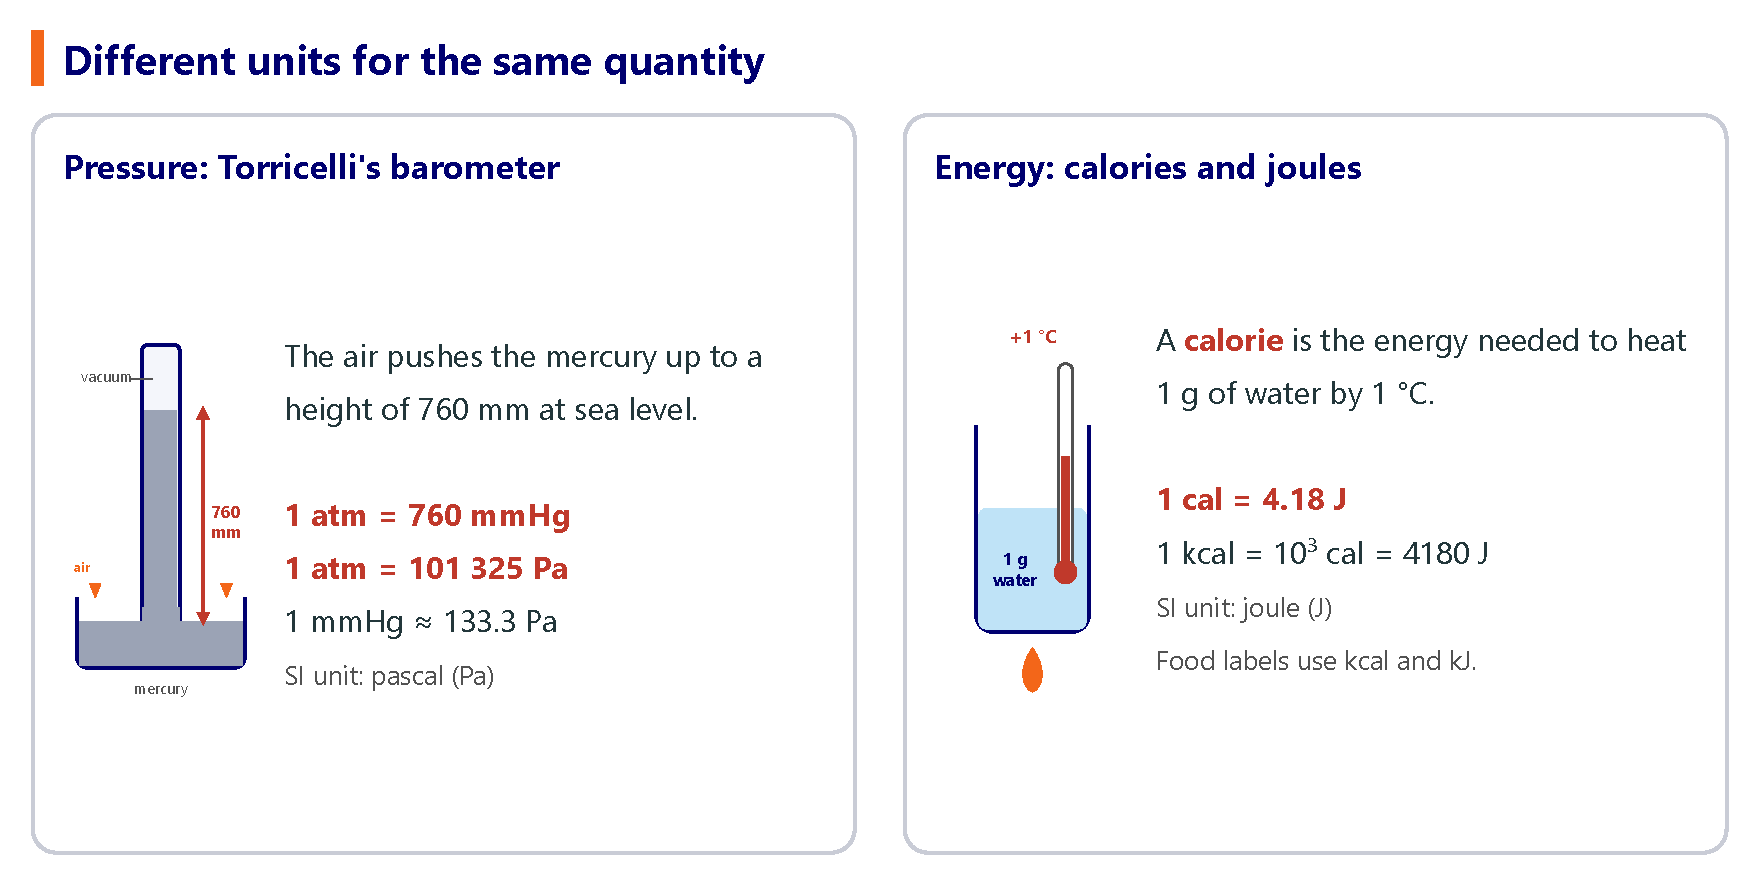
\includegraphics[width=\textwidth]{FigurasSVG/Unit_1_Matter_Measurement/pdf/pressure_energy.pdf}
    \caption{Where the atmosphere, the millimetre of mercury and the calorie come from.}
    \label{fig:u1_pressure_energy}
\end{figure}

\begin{table}[H]
    \centering
    \renewcommand{\arraystretch}{1.4}
    \begin{tabular}{lcp{6.5cm}}
        \toprule
        \textbf{Quantity} & \textbf{SI unit} & \textbf{Equivalences} \\
        \midrule
        Pressure & pascal (\unit{\Pa}) & \(\qty{1}{\atmospher} = \qty{760}{\mmhg}\) \newline \(\qty{1}{\atmospher} = \qty{101325}{\Pa} \approx \qty{1.013e5}{\Pa}\) \\
        Energy & joule (\unit{\J}) & \(\qty{1}{\calorie} = \qty{4.18}{\J}\) \newline \(\qty{1}{\kilo\calorie} = \qty{e3}{\calorie}\) \\
        \bottomrule
    \end{tabular}
    \caption{Units of pressure and energy and their equivalences.}
    \label{tab:u1_pressure_energy}
\end{table}

\begin{example}
    \textbf{Pressure.} The air pressure in a tyre is \qty{1.5}{\atmospher}. Write it in \unit{\Pa} and in \unit{\mmhg}.
    \begin{equation*}
        \num{1.5}\,\cancelunit{\atmospher} \cdot \dfrac{\qty{101325}{\Pa}}{1\,\cancelunit{\atmospher}} \approx \textcolor{red}{\qty{1.52e5}{\Pa}}
        \qquad\qquad
        \num{1.5}\,\cancelunit{\atmospher} \cdot \dfrac{\qty{760}{\mmhg}}{1\,\cancelunit{\atmospher}} = \textcolor{red}{\qty{1140}{\mmhg}}
    \end{equation*}
\end{example}

\begin{example}
    \textbf{Pressure.} Write \qty{380}{\mmhg} in pascals. There is no direct equivalence, so we go through atmospheres:
    \begin{equation*}
        \num{380}\,\cancelunit{\mmhg} \cdot \dfrac{1\,\cancelunit{\atmospher}}{\num{760}\,\cancelunit{\mmhg}} \cdot \dfrac{\qty{101325}{\Pa}}{1\,\cancelunit{\atmospher}} \approx \textcolor{red}{\qty{5.07e4}{\Pa}}
    \end{equation*}
\end{example}

\begin{example}
    \textbf{Energy.} A chocolate bar gives \qty{250}{\kilo\calorie}. Write this energy in joules.
    \begin{equation*}
        \num{250}\,\cancelunit{\kilo\calorie} \cdot \dfrac{\num{e3}\,\cancelunit{\calorie}}{1\,\cancelunit{\kilo\calorie}} \cdot \dfrac{\qty{4.18}{\J}}{1\,\cancelunit{\calorie}} = \textcolor{red}{\qty{1.045e6}{\J}}
    \end{equation*}
\end{example}

\begin{exercise}
    Convert these pressures:
    \begin{enumerate}[label=\letraminuscula]
        \item \qty{0.33}{\atmospher} (air pressure at the top of Mount Everest) to \unit{\mmhg}.
        \item \qty{120}{\mmhg} (a normal blood pressure) to \unit{\atmospher} and to \unit{\Pa}.
        \item \qty{2e5}{\Pa} to \unit{\atmospher}.
    \end{enumerate}
    \begin{solu}
        \begin{enumerate}[label=\alph*)]
            \item \(\num{0.33}\,\unit{\atmospher} \cdot \dfrac{\qty{760}{\mmhg}}{\qty{1}{\atmospher}} \approx \qty{251}{\mmhg}\)
            \item \(\num{120}\,\unit{\mmhg} \cdot \dfrac{\qty{1}{\atmospher}}{\qty{760}{\mmhg}} \approx \qty{0.158}{\atmospher}\); \quad
            \(\num{120}\,\unit{\mmhg} \cdot \dfrac{\qty{1}{\atmospher}}{\qty{760}{\mmhg}} \cdot \dfrac{\qty{101325}{\Pa}}{\qty{1}{\atmospher}} \approx \qty{1.60e4}{\Pa}\)
            \item \(\num{2e5}\,\unit{\Pa} \cdot \dfrac{\qty{1}{\atmospher}}{\qty{101325}{\Pa}} \approx \qty{1.97}{\atmospher}\)
        \end{enumerate}
    \end{solu}
\end{exercise}

\begin{exercise}
    Convert these energies:
    \begin{enumerate}[label=\letraminuscula]
        \item \qty{836}{\J} to calories.
        \item A yoghurt label says \qty{400}{\kilo\joule}. Write this energy in \unit{\kilo\calorie}.
        \item \qty{1.5}{\kilo\calorie} to \unit{\J}.
    \end{enumerate}
    \begin{solu}
        \begin{enumerate}[label=\alph*)]
            \item \(\num{836}\,\unit{\J} \cdot \dfrac{\qty{1}{\calorie}}{\qty{4.18}{\J}} = \qty{200}{\calorie}\)
            \item \(\num{400}\,\unit{\kilo\joule} \cdot \dfrac{\qty{e3}{\J}}{\qty{1}{\kilo\joule}} \cdot \dfrac{\qty{1}{\calorie}}{\qty{4.18}{\J}} \cdot \dfrac{\qty{1}{\kilo\calorie}}{\qty{e3}{\calorie}} \approx \qty{95.7}{\kilo\calorie}\)
            \item \(\num{1.5}\,\unit{\kilo\calorie} \cdot \dfrac{\qty{e3}{\calorie}}{\qty{1}{\kilo\calorie}} \cdot \dfrac{\qty{4.18}{\J}}{\qty{1}{\calorie}} = \qty{6270}{\J}\)
        \end{enumerate}
    \end{solu}
\end{exercise}

%----------------------------------------------------------------------------------------

\subsection{Scientific notation}

% Calculator keys: \calckey{EXP} draws one key; \keys{3 . 2 EXP 3} draws one key per word
\providecommand{\calckey}[1]{{\setlength{\fboxsep}{1.5pt}\fbox{\footnotesize\sffamily\strut #1}}}
\ExplSyntaxOn
\providecommand{\keys}[1]{\seq_set_split:Nnn \l_tmpa_seq {~} {#1} \seq_map_inline:Nn \l_tmpa_seq {\calckey{##1}\,} \unskip}
\ExplSyntaxOff
% Red decimal comma used to show where the comma ends up in the examples
\providecommand{\redcomma}{\textcolor{red}{\mathbf{,}}}

In science we often find numbers that are very big or very small. The distance from the Earth to the Sun is about \qty{150000000}{\km}, and a bacterium measures about \qty{0.000002}{\m}. Writing and reading so many zeros is slow and it is very easy to make mistakes. That is why scientists use \negsubro{scientific notation}. You have already used it with conversion factors: \(\qty{1}{\km} = \qty{e3}{\m}\).

\begin{definition}[Scientific notation]
    A way of writing a number as the product of a \textbf{coefficient} and a \textbf{power of 10}:
    \begin{equation*}
        a \cdot 10^{n}
    \end{equation*}
    \begin{itemize}
        \item The \textbf{coefficient} \(a\) is a number from 1 to 9,99\ldots: it has \textbf{only one digit, different from zero, before the decimal comma}.
        \item The \textbf{exponent} \(n\) is a whole number: \textbf{positive} for numbers greater than 10, and \textbf{negative} for numbers smaller than 1.
    \end{itemize}
\end{definition}

\begin{figure}[H]
    \centering
    % [FIGURA ORIGINAL] \includegraphics[width=\textwidth]{Unit_1/sci_notation_parts}
    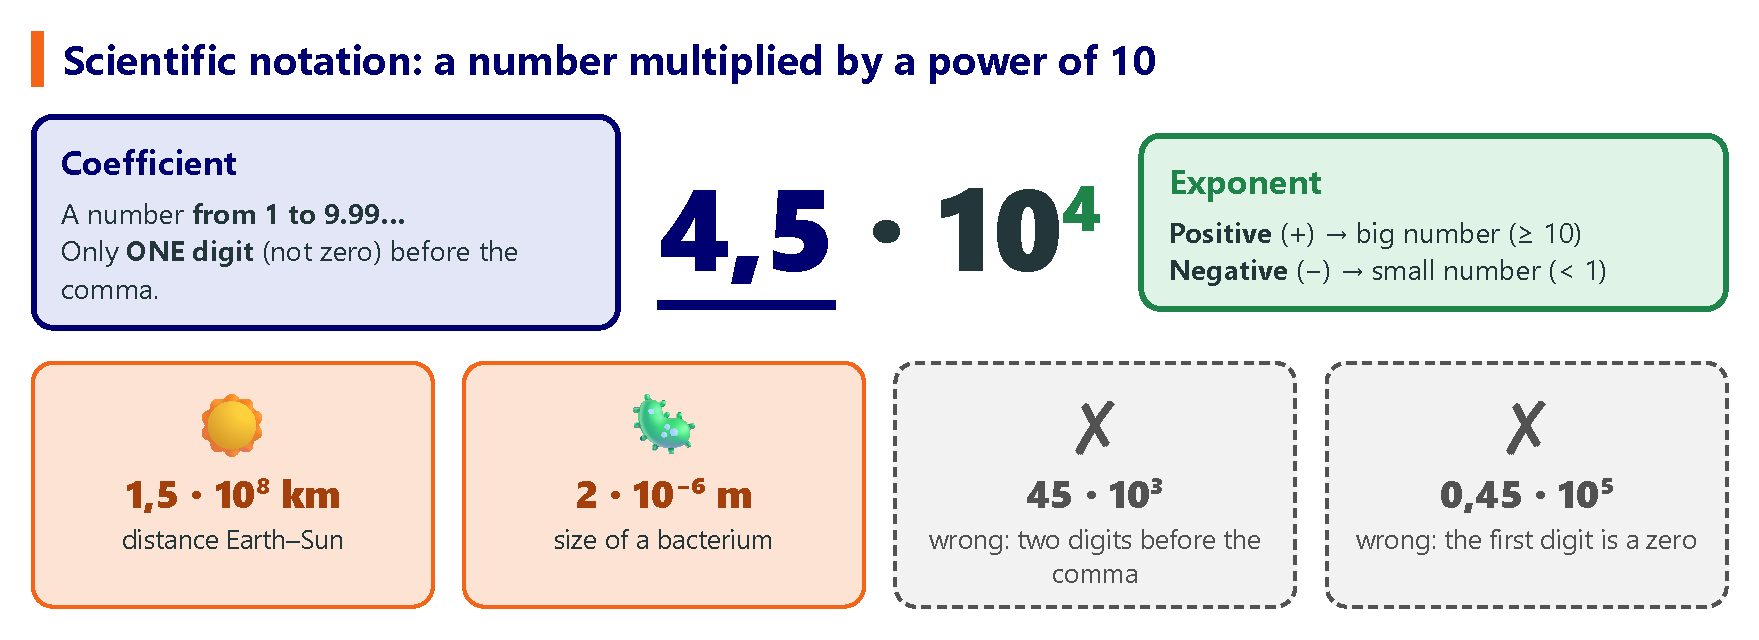
\includegraphics[width=\textwidth]{FigurasSVG/Unit_1_Matter_Measurement/pdf/sci_notation_parts.pdf}
    \caption{The two parts of a number in scientific notation, with correct and incorrect examples.}
    \label{fig:u1_sci_notation_parts}
\end{figure}

\begin{impt}
    \negsubro{Scientific notation does not change the number!} It is the \textbf{same number written in a different way}, just as ``a half'', \(\frac{1}{2}\) and \(0{,}5\) are the same amount:
    \begin{equation*}
        45\,000 = 4{,}5 \cdot 10^{4} = 45 \cdot 10^{3} = 450 \cdot 10^{2} = 0{,}45 \cdot 10^{5}
    \end{equation*}
    All of them are worth exactly the same. Of all these ways of writing it, only \(4{,}5 \cdot 10^{4}\) is \textbf{correct scientific notation}, because it has only one digit (different from zero) before the comma.
\end{impt}

Remember what a power of 10 means: the exponent tells us how many places the comma moves.

\begin{table}[H]
    \centering
    \renewcommand{\arraystretch}{1.35}
    \begin{tabular}{cc@{\hspace{1.5cm}}cc}
        \toprule
        \textbf{Power} & \textbf{Decimal} & \textbf{Power} & \textbf{Decimal} \\
        \midrule
        \(10^{1}\) & \num{10}    & \(10^{-1}\) & \num{0.1}   \\
        \(10^{2}\) & \num{100}   & \(10^{-2}\) & \num{0.01}  \\
        \(10^{3}\) & \num{1000}  & \(10^{-3}\) & \num{0.001} \\
        \(10^{4}\) & \num{10000} & \(10^{-4}\) & \num{0.0001} \\
        \bottomrule
    \end{tabular}
    \caption{Positive powers of 10 are numbers \textbf{greater than 1}; negative powers of 10 are numbers \textbf{smaller than 1}. \(10^{0} = 1\).}
    \label{tab:u1_powers_of_ten}
\end{table}

\begin{figure}[H]
    \centering
    % [FIGURA ORIGINAL] \includegraphics[width=\textwidth]{Unit_1/sci_notation_to}
    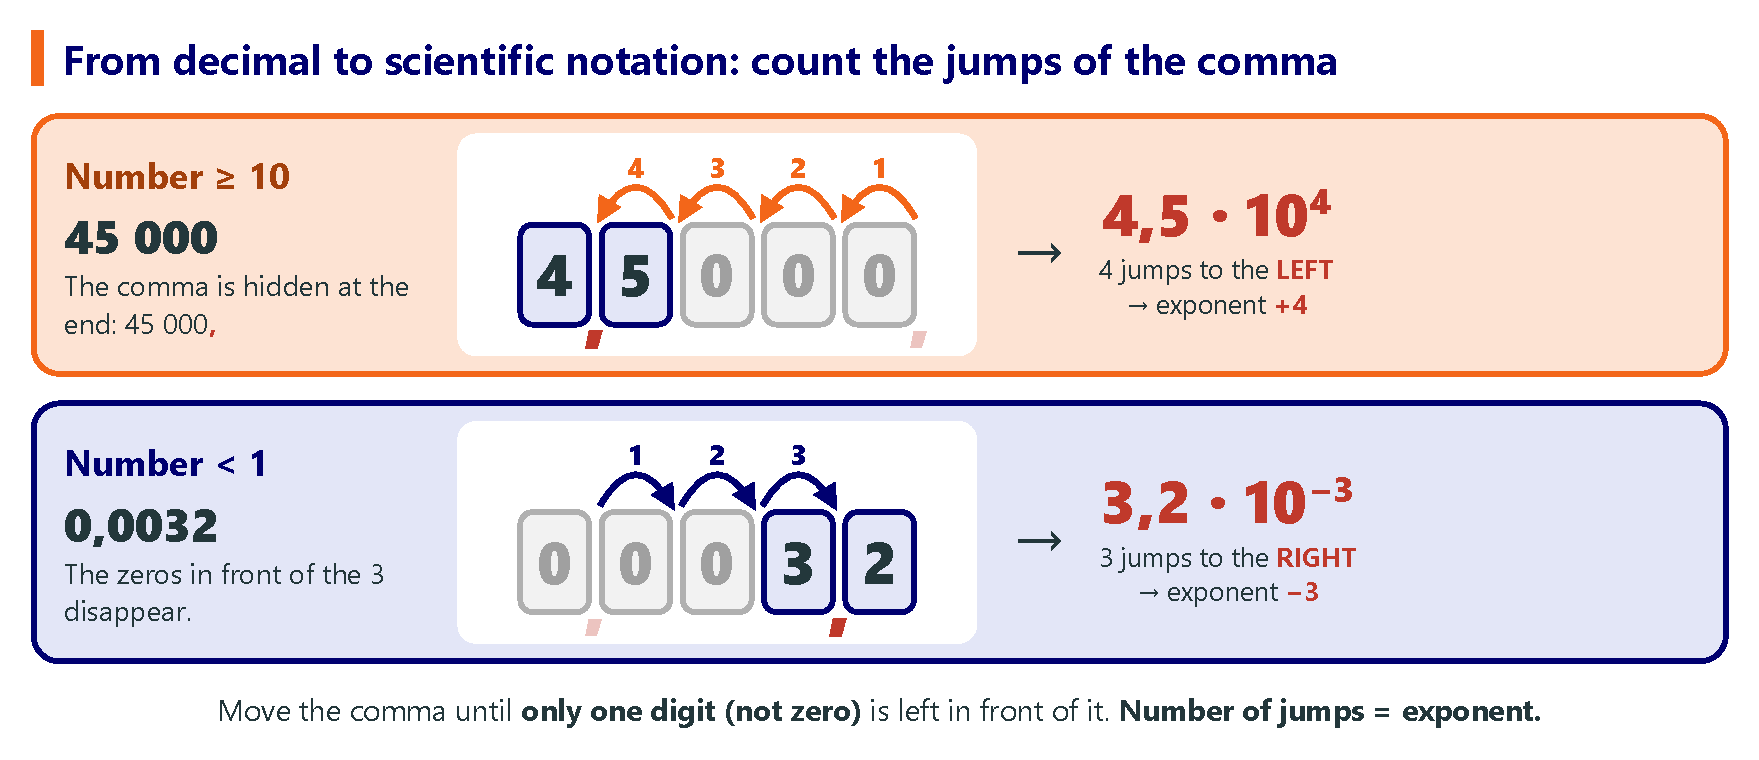
\includegraphics[width=\textwidth]{FigurasSVG/Unit_1_Matter_Measurement/pdf/sci_notation_to.pdf}
    \caption{To write a number in scientific notation we count how many places the comma jumps.}
    \label{fig:u1_sci_notation_to}
\end{figure}

%------------------------------------------------

\subsubsection{Numbers greater than 1 to scientific notation}

\negsubro{Method, step by step}:
\begin{enumerate}[label=\numberballmDarkTeal]
    \item Find the decimal comma. If the number has no comma, it is \textbf{hidden at the end}: \(45\,000 = 45\,000\redcomma\)
    \item Move the comma to the \textbf{left}, one place at a time, until \textbf{only one digit} is left in front of it. \textbf{Count the jumps}.
    \item Write the \textbf{coefficient}: the digits with the comma in its new place. The zeros at the end are not needed: \(4\redcomma 5000 = 4{,}5\).
    \item The \textbf{exponent} is the \textbf{number of jumps}, and it is \textbf{positive}: the number was big.
    \item Check: \(\num{4.5e4}\) must be equal to the starting number.
\end{enumerate}

\begin{example}
    \textbf{Write \num{45000} in scientific notation.}
    \begin{enumerate}[label=\numberballmDarkTeal]
        \item Hidden comma at the end: \(45\,000\redcomma\)
        \item We move the comma 4 places to the left: \(45\,000\redcomma \to 4500\redcomma 0 \to 450\redcomma 00 \to 45\redcomma 000 \to 4\redcomma 5000\) \(\Rightarrow\) \textbf{4 jumps}.
        \item Coefficient: \(4{,}5\).
        \item Exponent: \(+4\).
        \item \(\textcolor{red}{\num{45000} = \num{4.5e4}}\)
    \end{enumerate}
\end{example}

\begin{example}
    \textbf{Write \num{6700} and \num{380.5} in scientific notation.}
    \begin{itemize}
        \item \(6700\redcomma \to 6\redcomma 700\): 3 jumps to the left \(\Rightarrow\) \(\textcolor{red}{\num{6700} = \num{6.7e3}}\)
        \item \(380{,}5 \to 3\redcomma 805\): 2 jumps to the left \(\Rightarrow\) \(\textcolor{red}{\num{380.5} = \num{3.805e2}}\)
    \end{itemize}
\end{example}

%------------------------------------------------

\subsubsection{Numbers smaller than 1 to scientific notation}

\negsubro{Method, step by step}:
\begin{enumerate}[label=\numberballmDarkTeal]
    \item Find the decimal comma: \(0{,}0032\).
    \item Move the comma to the \textbf{right}, one place at a time, until it is just after the \textbf{first digit that is not zero}. \textbf{Count the jumps}.
    \item Write the \textbf{coefficient}: the zeros in front disappear: \(0003\redcomma 2 = 3{,}2\).
    \item The \textbf{exponent} is the \textbf{number of jumps}, and it is \textbf{negative}: the number was smaller than 1.
    \item Check: \(\num{3.2e-3}\) must be equal to the starting number.
\end{enumerate}

\begin{example}
    \textbf{Write \num{0.0032} in scientific notation.}
    \begin{enumerate}[label=\numberballmDarkTeal]
        \item Comma: \(0\redcomma 0032\)
        \item We move the comma 3 places to the right: \(0\redcomma 0032 \to 00\redcomma 032 \to 000\redcomma 32 \to 0003\redcomma 2\) \(\Rightarrow\) \textbf{3 jumps}.
        \item Coefficient: \(3{,}2\).
        \item Exponent: \(-3\).
        \item \(\textcolor{red}{\num{0.0032} = \num{3.2e-3}}\)
    \end{enumerate}
\end{example}

\begin{example}
    \textbf{Write \num{0.07} and \num{0.125} in scientific notation.}
    \begin{itemize}
        \item \(0{,}07 \to 007\redcomma\): 2 jumps to the right \(\Rightarrow\) \(\textcolor{red}{\num{0.07} = \num{7e-2}}\)
        \item \(0{,}125 \to 01\redcomma 25\): 1 jump to the right \(\Rightarrow\) \(\textcolor{red}{\num{0.125} = \num{1.25e-1}}\)
    \end{itemize}
\end{example}

\begin{impt}
    \textbf{Which way does the comma move?}
    \begin{itemize}
        \item Big number (greater than 10) \(\to\) the comma jumps to the \textbf{left} \(\to\) exponent \textbf{positive}.
        \item Small number (smaller than 1) \(\to\) the comma jumps to the \textbf{right} \(\to\) exponent \textbf{negative}.
        \item Number between 1 and 10 \(\to\) the comma does not move \(\to\) exponent \textbf{0}: \(7{,}2 = \num{7.2e0}\).
    \end{itemize}
\end{impt}

%------------------------------------------------

\subsubsection{From scientific notation to decimal}

Now we do the opposite: we start from \(a \cdot 10^{n}\) and we want the normal (decimal) number. The \textbf{exponent} tells us how many places the comma jumps, and its \textbf{sign} tells us in which direction.

\begin{figure}[H]
    \centering
    % [FIGURA ORIGINAL] \includegraphics[width=\textwidth]{Unit_1/sci_notation_back}
    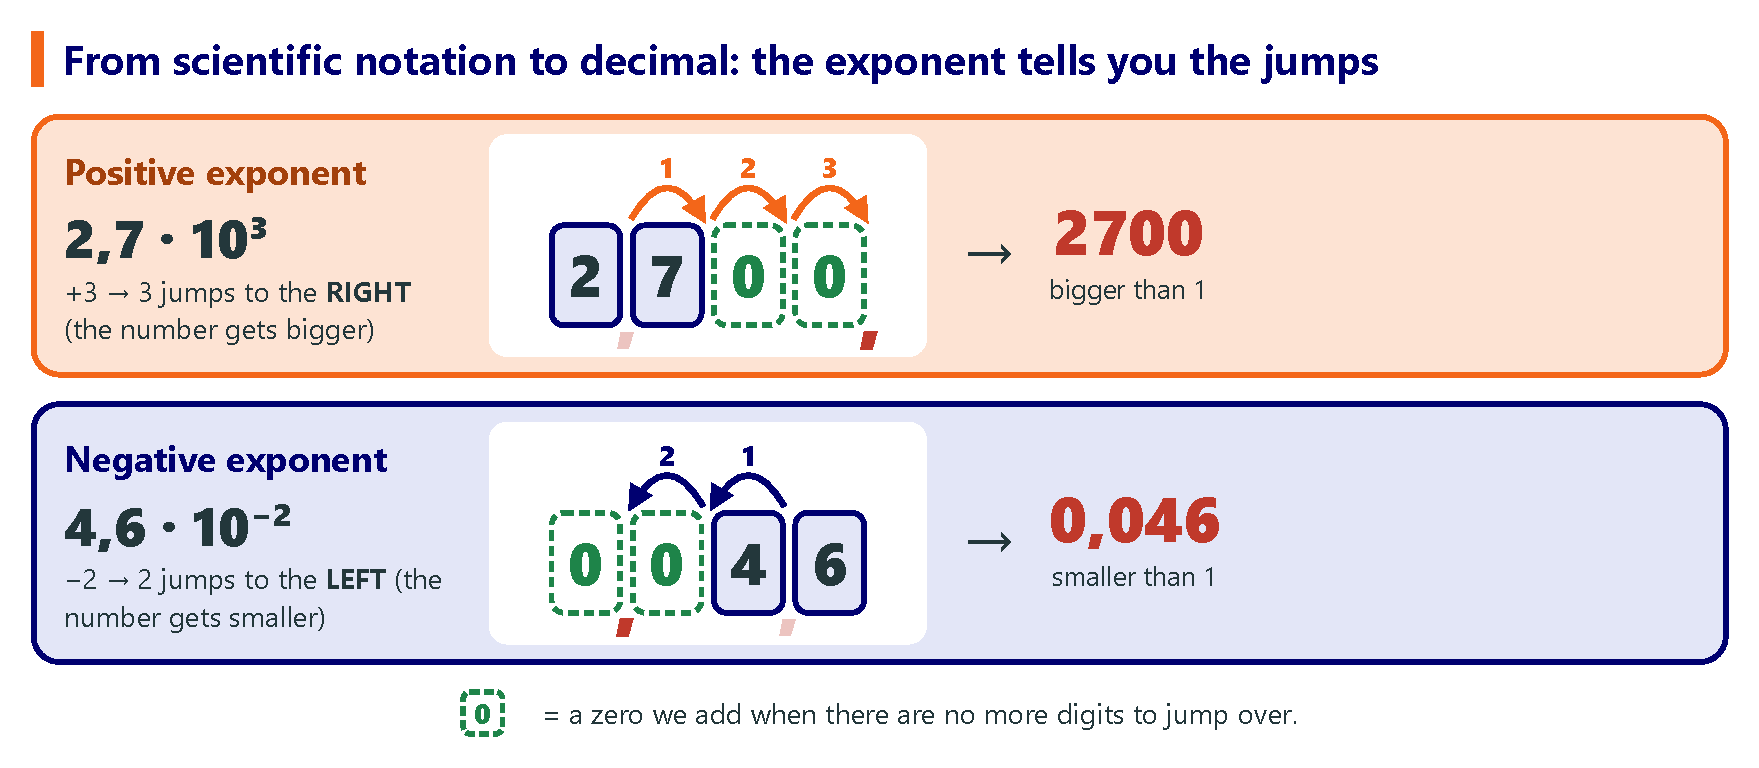
\includegraphics[width=\textwidth]{FigurasSVG/Unit_1_Matter_Measurement/pdf/sci_notation_back.pdf}
    \caption{From scientific notation to decimal: positive exponent, the comma jumps to the right; negative exponent, the comma jumps to the left.}
    \label{fig:u1_sci_notation_back}
\end{figure}

\negsubro{Method, step by step}:
\begin{enumerate}[label=\numberballmDarkTeal]
    \item Look at the \textbf{sign of the exponent}:
    \begin{itemize}
        \item \textbf{Positive} \(\to\) the comma jumps to the \textbf{right} (the number gets \textbf{bigger}).
        \item \textbf{Negative} \(\to\) the comma jumps to the \textbf{left} (the number gets \textbf{smaller}).
    \end{itemize}
    \item Move the comma as many places as the exponent says.
    \item If there are no more digits to jump over, \textbf{add zeros}.
    \item If the comma ends up at the very front, write a \textbf{0} before it: \(\redcomma 046 \to 0{,}046\).
\end{enumerate}

\begin{example}
    \textbf{Positive exponent: write \num{2.7e3} as a decimal number.}
    \begin{enumerate}[label=\numberballmDarkTeal]
        \item Exponent \(+3\): 3 jumps to the \textbf{right}.
        \item \(2\redcomma 7 \to 27\redcomma \to 270\redcomma \to 2700\redcomma\) (we have added two zeros).
        \item \(\textcolor{red}{\num{2.7e3} = \num{2700}}\)
    \end{enumerate}
    More examples: \(\num{5e2} = 500\); \quad \(\num{1.25e3} = 1250\); \quad \(\num{3.06e4} = \num{30600}\).
\end{example}

\begin{example}
    \textbf{Negative exponent: write \num{4.6e-2} as a decimal number.}
    \begin{enumerate}[label=\numberballmDarkTeal]
        \item Exponent \(-2\): 2 jumps to the \textbf{left}.
        \item \(4\redcomma 6 \to \redcomma 46 \to \redcomma 046\) (we have added one zero).
        \item We write a 0 in front of the comma: \(\textcolor{red}{\num{4.6e-2} = \num{0.046}}\)
    \end{enumerate}
    More examples: \(\num{8e-3} = \num{0.008}\); \quad \(\num{1.5e-1} = \num{0.15}\); \quad \(\num{9.2e-4} = \num{0.00092}\).
\end{example}

\begin{marker}
    \textbf{Quick check}: if the exponent is positive, your decimal number must be \textbf{greater than 1}; if it is negative, it must start with \textbf{0,\ldots}. If not, you moved the comma in the wrong direction!
\end{marker}

\begin{exercise}
    Write these numbers in scientific notation:
    \begin{enumerate}[label=\letraminuscula]
        \item \num{3400}
        \item \num{52000}
        \item \num{700000}
        \item \num{186}
        \item \num{0.045}
        \item \num{0.0007}
        \item \num{0.00128}
        \item \num{0.5}
    \end{enumerate}
    \begin{solu}
        \begin{enumerate}[label=\alph*)]
            \item 3 jumps to the left: \(\num{3.4e3}\)
            \item 4 jumps to the left: \(\num{5.2e4}\)
            \item 5 jumps to the left: \(\num{7e5}\)
            \item 2 jumps to the left: \(\num{1.86e2}\)
            \item 2 jumps to the right: \(\num{4.5e-2}\)
            \item 4 jumps to the right: \(\num{7e-4}\)
            \item 3 jumps to the right: \(\num{1.28e-3}\)
            \item 1 jump to the right: \(\num{5e-1}\)
        \end{enumerate}
    \end{solu}
\end{exercise}

\begin{exercise}
    Write these numbers as decimal numbers:
    \begin{enumerate}[label=\letraminuscula]
        \item \num{3.1e2}
        \item \num{6e4}
        \item \num{1.25e3}
        \item \num{9e-1}
        \item \num{2.4e-3}
        \item \num{7.05e-2}
    \end{enumerate}
    \begin{solu}
        \begin{enumerate}[label=\alph*)]
            \item 2 jumps to the right: \num{310}
            \item 4 jumps to the right: \num{60000}
            \item 3 jumps to the right: \num{1250}
            \item 1 jump to the left: \num{0.9}
            \item 3 jumps to the left: \num{0.0024}
            \item 2 jumps to the left: \num{0.0705}
        \end{enumerate}
    \end{solu}
\end{exercise}

\begin{exercise}
    These numbers are \textbf{not} correctly written in scientific notation. Explain the mistake and write them correctly: \num{23e4}, \num{0.8e3}, \num{15e-3}.
    \begin{solu}
        \begin{itemize}
            \item \(\num{23e4}\): two digits before the comma. \(\num{23e4} = \num{230000} = \num{2.3e5}\).
            \item \(\num{0.8e3}\): the digit before the comma is a zero. \(\num{0.8e3} = \num{800} = \num{8e2}\).
            \item \(\num{15e-3}\): two digits before the comma. \(\num{15e-3} = \num{0.015} = \num{1.5e-2}\).
        \end{itemize}
    \end{solu}
\end{exercise}

\begin{exercise}
    Write the numbers in these sentences in scientific notation:
    \begin{enumerate}[label=\letraminuscula]
        \item Sound travels through air at \qty{340}{\m\per\s}.
        \item A human hair is about \qty{0.00008}{\m} thick.
        \item The Moon is about \qty{384000}{\km} away from the Earth.
        \item A grain of sand has a mass of about \qty{0.0006}{\g}.
    \end{enumerate}
    \begin{solu}
        \begin{enumerate}[label=\alph*)]
            \item \(\qty{3.4e2}{\m\per\s}\)
            \item \(\qty{8e-5}{\m}\)
            \item \(\qty{3.84e5}{\km}\)
            \item \(\qty{6e-4}{\g}\)
        \end{enumerate}
    \end{solu}
\end{exercise}

\begin{exercise}
    Write these numbers in scientific notation. Be careful: the last four already have a power of 10, but they are \textbf{not} correctly written yet.
    \begin{enumerate}[label=\letraminuscula]
        \item \num{4569201}
        \item \num{0.0026}
        \item \num{235.78}
        \item \num{500000}
        \item \num{4055e4}
        \item \num{5687e-8}
        \item \num{253e8}
        \item \num{0.0254e-2}
    \end{enumerate}
    \begin{solu}
        \begin{enumerate}[label=\alph*)]
            \item 6 jumps to the left: \(\num{4.569201e6}\)
            \item 3 jumps to the right: \(\num{2.6e-3}\)
            \item 2 jumps to the left: \(\num{2.3578e2}\)
            \item 5 jumps to the left: \(\num{5e5}\)
            \item \(4055 = \num{4.055e3}\), so \(\num{4055e4} = \num{4.055e3} \cdot 10^{4} = \num{4.055e7}\)
            \item \(5687 = \num{5.687e3}\), so \(\num{5687e-8} = \num{5.687e3} \cdot 10^{-8} = \num{5.687e-5}\)
            \item \(253 = \num{2.53e2}\), so \(\num{253e8} = \num{2.53e2} \cdot 10^{8} = \num{2.53e10}\)
            \item \(0{,}0254 = \num{2.54e-2}\), so \(\num{0.0254e-2} = \num{2.54e-2} \cdot 10^{-2} = \num{2.54e-4}\)
        \end{enumerate}
    \end{solu}
\end{exercise}

%------------------------------------------------

\subsubsection{Scientific notation on the calculator}

Every scientific calculator has a special key to write a power of 10. Depending on how old the calculator is, it is called \textbf{EXP} or \(\boldsymbol{\times 10^{x}}\), but it does exactly the same: it means ``\(\times\,10\) to the power of''. Look for your calculator in the figure and follow the keys.

\begin{figure}[H]
    \centering
    % [FIGURA ORIGINAL] \includegraphics[width=\textwidth]{Unit_1/calculators_sci}
    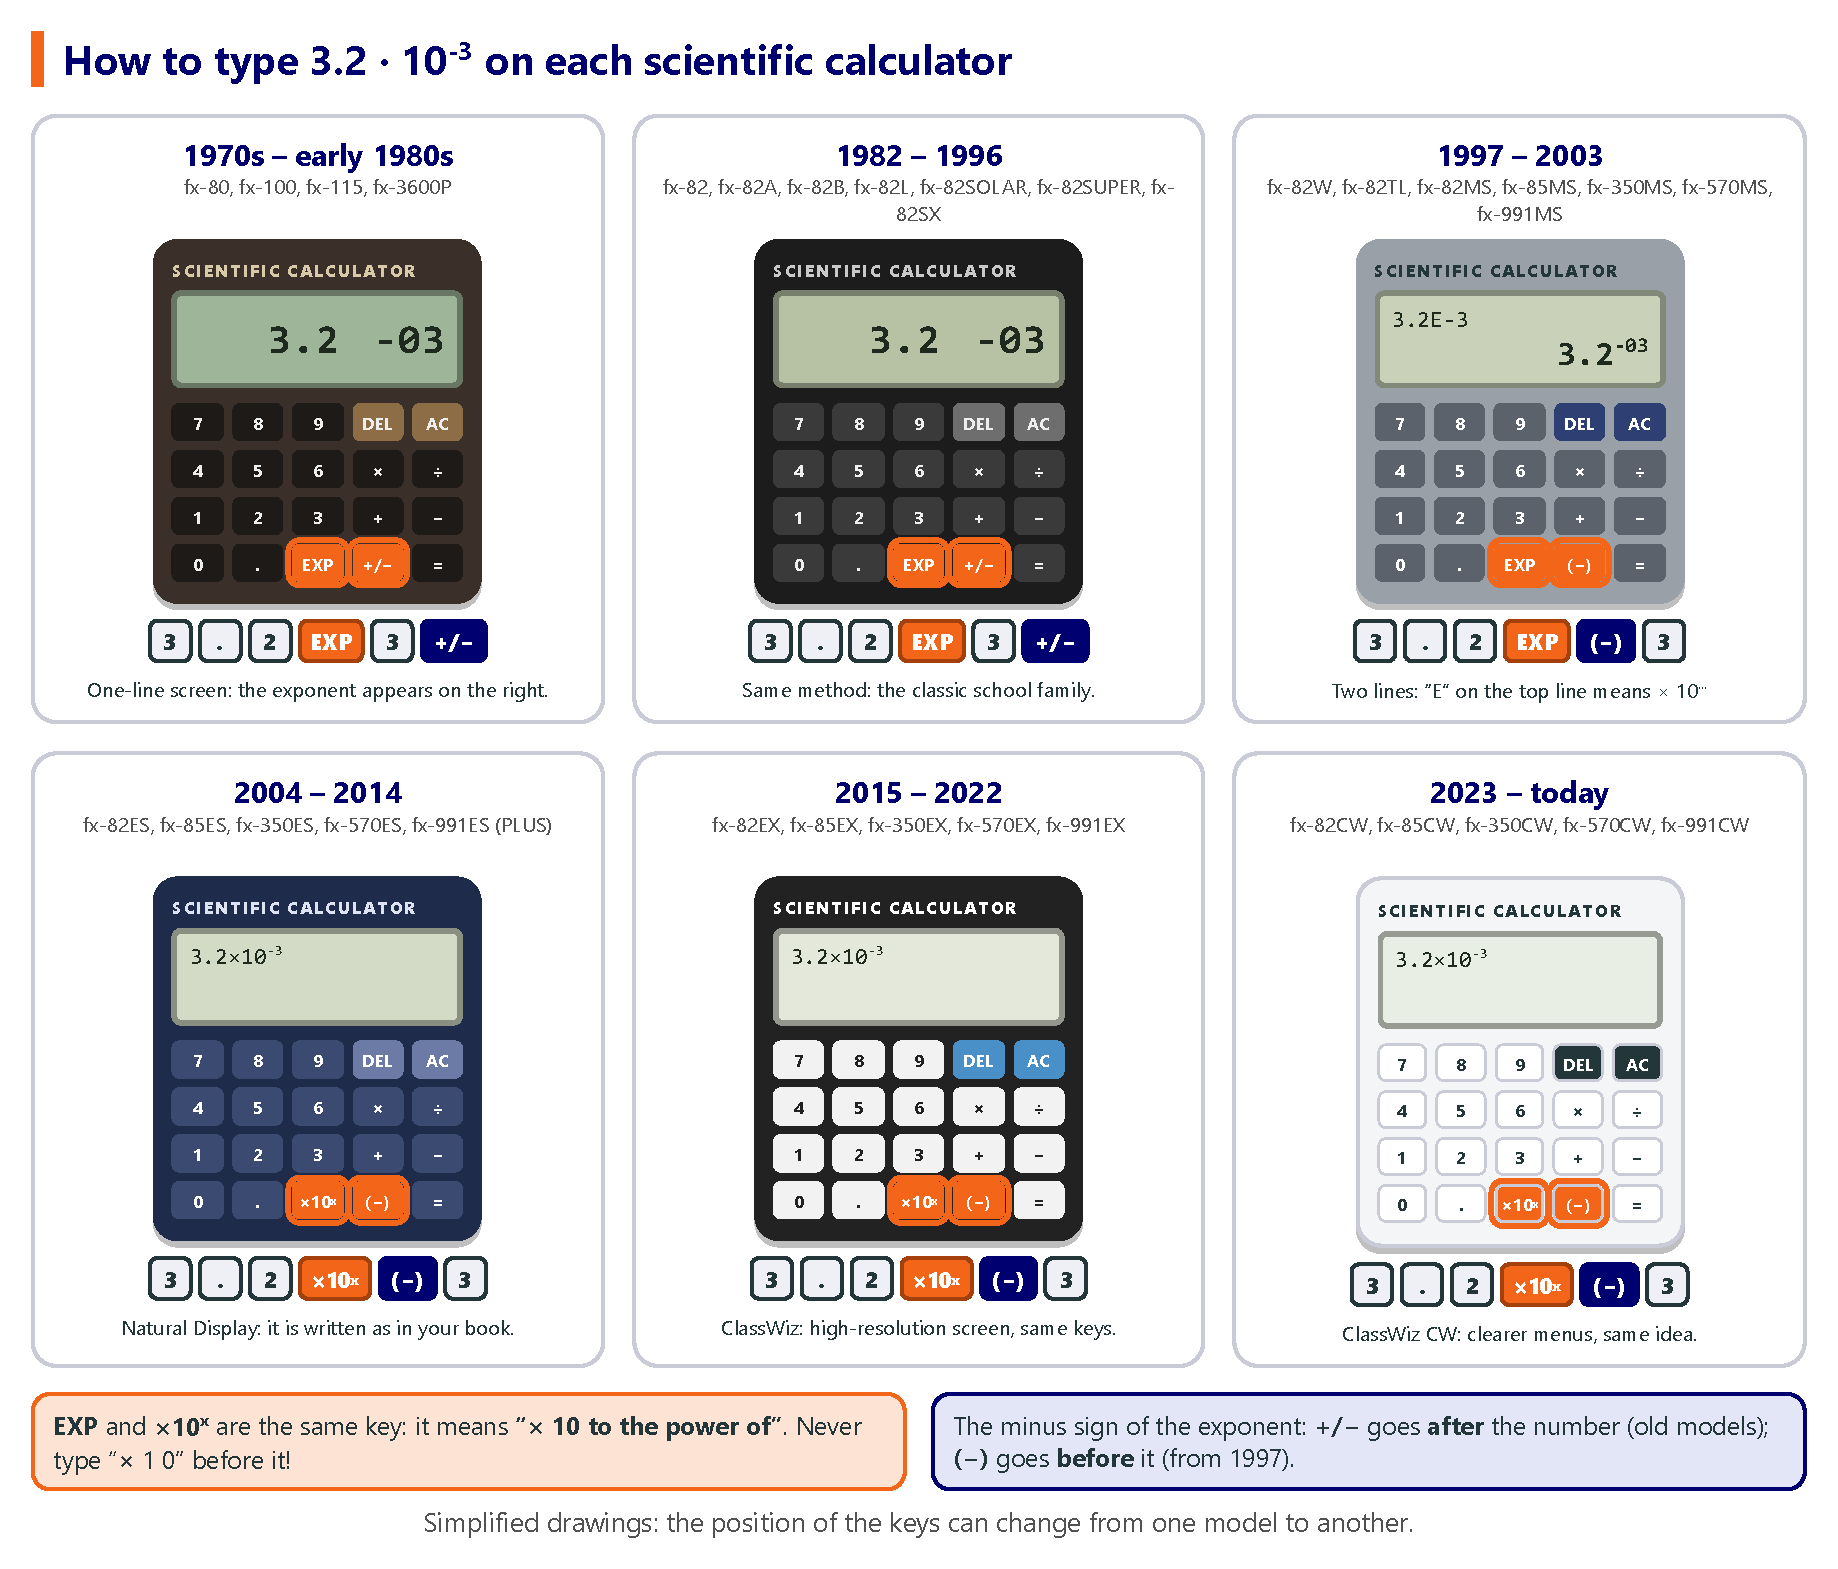
\includegraphics[width=\textwidth]{FigurasSVG/Unit_1_Matter_Measurement/pdf/calculators_sci.pdf}
    \caption{How to type \(\num{3.2e-3}\) on the scientific calculators used in schools over the years (simplified drawings).}
    \label{fig:u1_calculators_sci}
\end{figure}

\begin{table}[H]
    \centering
    \small
    \renewcommand{\arraystretch}{1.35}
    \begin{tabular}{p{1.9cm}p{4.0cm}p{2.9cm}p{3.7cm}}
        \toprule
        \textbf{Years} & \textbf{Most common models} & \textbf{Keys} & \textbf{To type \(\num{3.2e-3}\)} \\
        \midrule
        1970s--early 1980s & fx-80, fx-100, fx-115, fx-3600P & \calckey{EXP} and \calckey{+/\(-\)} & \keys{3 . 2 EXP 3 +/-} \\
        1982--1996 & fx-82, fx-82A, fx-82B, fx-82L, fx-82SOLAR, fx-82SUPER, fx-82SX & \calckey{EXP} and \calckey{+/\(-\)} & \keys{3 . 2 EXP 3 +/-} \\
        1997--2003 & fx-82W, fx-82TL, fx-82MS, fx-85W, fx-85MS, fx-115W, fx-115MS, fx-350MS, fx-570MS, fx-991MS & \calckey{EXP} and \calckey{(\(-\))} & \keys{3 . 2 EXP (-) 3} \\
        2004--2014 & fx-82ES, fx-85ES, fx-350ES, fx-570ES, fx-991ES, fx-82ES PLUS, fx-991ES PLUS & \calckey{\(\times10^{x}\)} and \calckey{(\(-\))} & \keys{3 . 2 \(\times10^{x}\) (-) 3} \\
        2015--2022 & fx-82EX, fx-85EX, fx-350EX, fx-570EX, fx-991EX (and 2nd edition) & \calckey{\(\times10^{x}\)} and \calckey{(\(-\))} & \keys{3 . 2 \(\times10^{x}\) (-) 3} \\
        2023--today & fx-82CW, fx-85CW, fx-350CW, fx-570CW, fx-991CW & \calckey{\(\times10^{x}\)} and \calckey{(\(-\))} & \keys{3 . 2 \(\times10^{x}\) (-) 3} \\
        \bottomrule
    \end{tabular}
    \caption{The scientific-notation key on the most common school calculators.}
    \label{tab:u1_calculators}
\end{table}

\begin{example}
    \textbf{Type \(\num{6.02e23}\)} (positive exponent, so no minus sign is needed):
    \begin{itemize}
        \item Calculators up to 2003: \keys{6 . 0 2 EXP 2 3}. On the screen you will see \texttt{6.02E23} or \(6.02^{23}\).
        \item Calculators from 2004 on: \keys{6 . 0 2 \(\times10^{x}\) 2 3}. On the screen you will see \(6.02 \times 10^{23}\).
    \end{itemize}
\end{example}

\begin{marker}
    \textbf{Typical mistake}: do \textbf{not} press \keys{\(\times\) 1 0} before the EXP or \(\times 10^{x}\) key, because the key already includes the ``\(\times\,10\)''. If you type \keys{3 . 2 \(\times\) 1 0 EXP (-) 3}, the calculator understands \(3{,}2 \cdot 10 \cdot 10^{-3}\), which is 10 times bigger! In the same way, to type \(10^{5}\) alone, press \keys{1 EXP 5}, not \keys{1 0 EXP 5}.
\end{marker}

\begin{exercise}
    Write the keys you would press on \textbf{your own} calculator to type these numbers, and check them on the screen: \textbf{a)} \(\num{5.4e6}\); \textbf{b)} \(\num{7.1e-4}\); \textbf{c)} \(\num{1.6e-19}\); \textbf{d)} \(\num{3e8}\).
    \begin{solu}
        With a calculator from 2004 on (with older ones, use EXP instead of \(\times 10^{x}\); before 1997, press \(+/-\) after the exponent instead of \((-)\) before it):
        a) \keys{5 . 4 \(\times10^{x}\) 6}; b) \keys{7 . 1 \(\times10^{x}\) (-) 4}; c) \keys{1 . 6 \(\times10^{x}\) (-) 1 9}; d) \keys{3 \(\times10^{x}\) 8}.
    \end{solu}
\end{exercise}


\section{Density and floating}


\begin{definition}[Density]
    The mass contained in each unit of volume of a substance:
    \begin{equation*}
        d = \dfrac{m}{V}
    \end{equation*}
\end{definition}

\begin{figure}[H]
    \centering
    % [FIGURA ORIGINAL] \includegraphics[width=\textwidth]{Unit_1/density_cubes}
    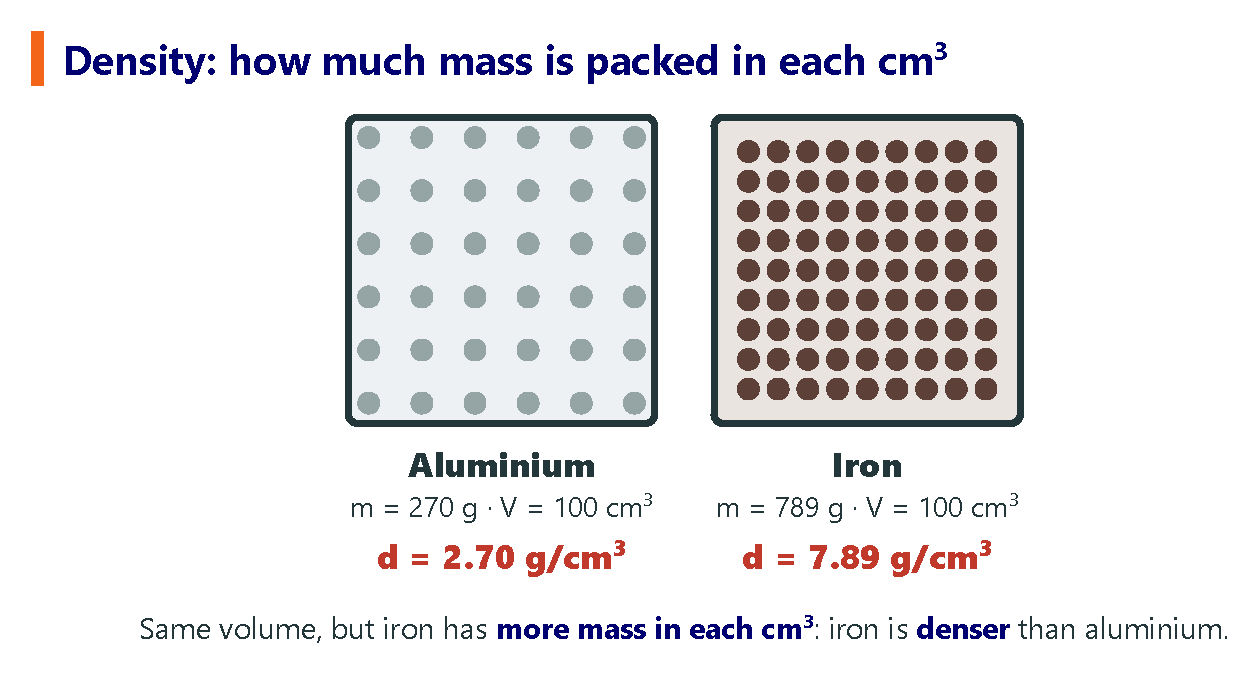
\includegraphics[width=\textwidth]{FigurasSVG/Unit_1_Matter_Measurement/pdf/density_cubes.pdf}
    \caption{Two cubes with the same volume but different mass have different densities.}
    \label{fig:u1_density_cubes}
\end{figure}

\negsubro{How to isolate a quantity in the density formula}

The formula \(d = \dfrac{m}{V}\) links three quantities. If we know \textbf{two} of them, we can always calculate the \textbf{third} one. But first we must leave the quantity we want to calculate \textbf{alone} on one side of the equals sign. This is called \textbf{isolating} (or rearranging) a quantity.

The key idea is that an equation is like a \textbf{balanced scale}: whatever we do to one side, we must also do to the other side, so that both sides stay equal.

\begin{figure}[H]
    \centering
    % [FIGURA ORIGINAL] \includegraphics[width=\textwidth]{Unit_1/density_isolate}
    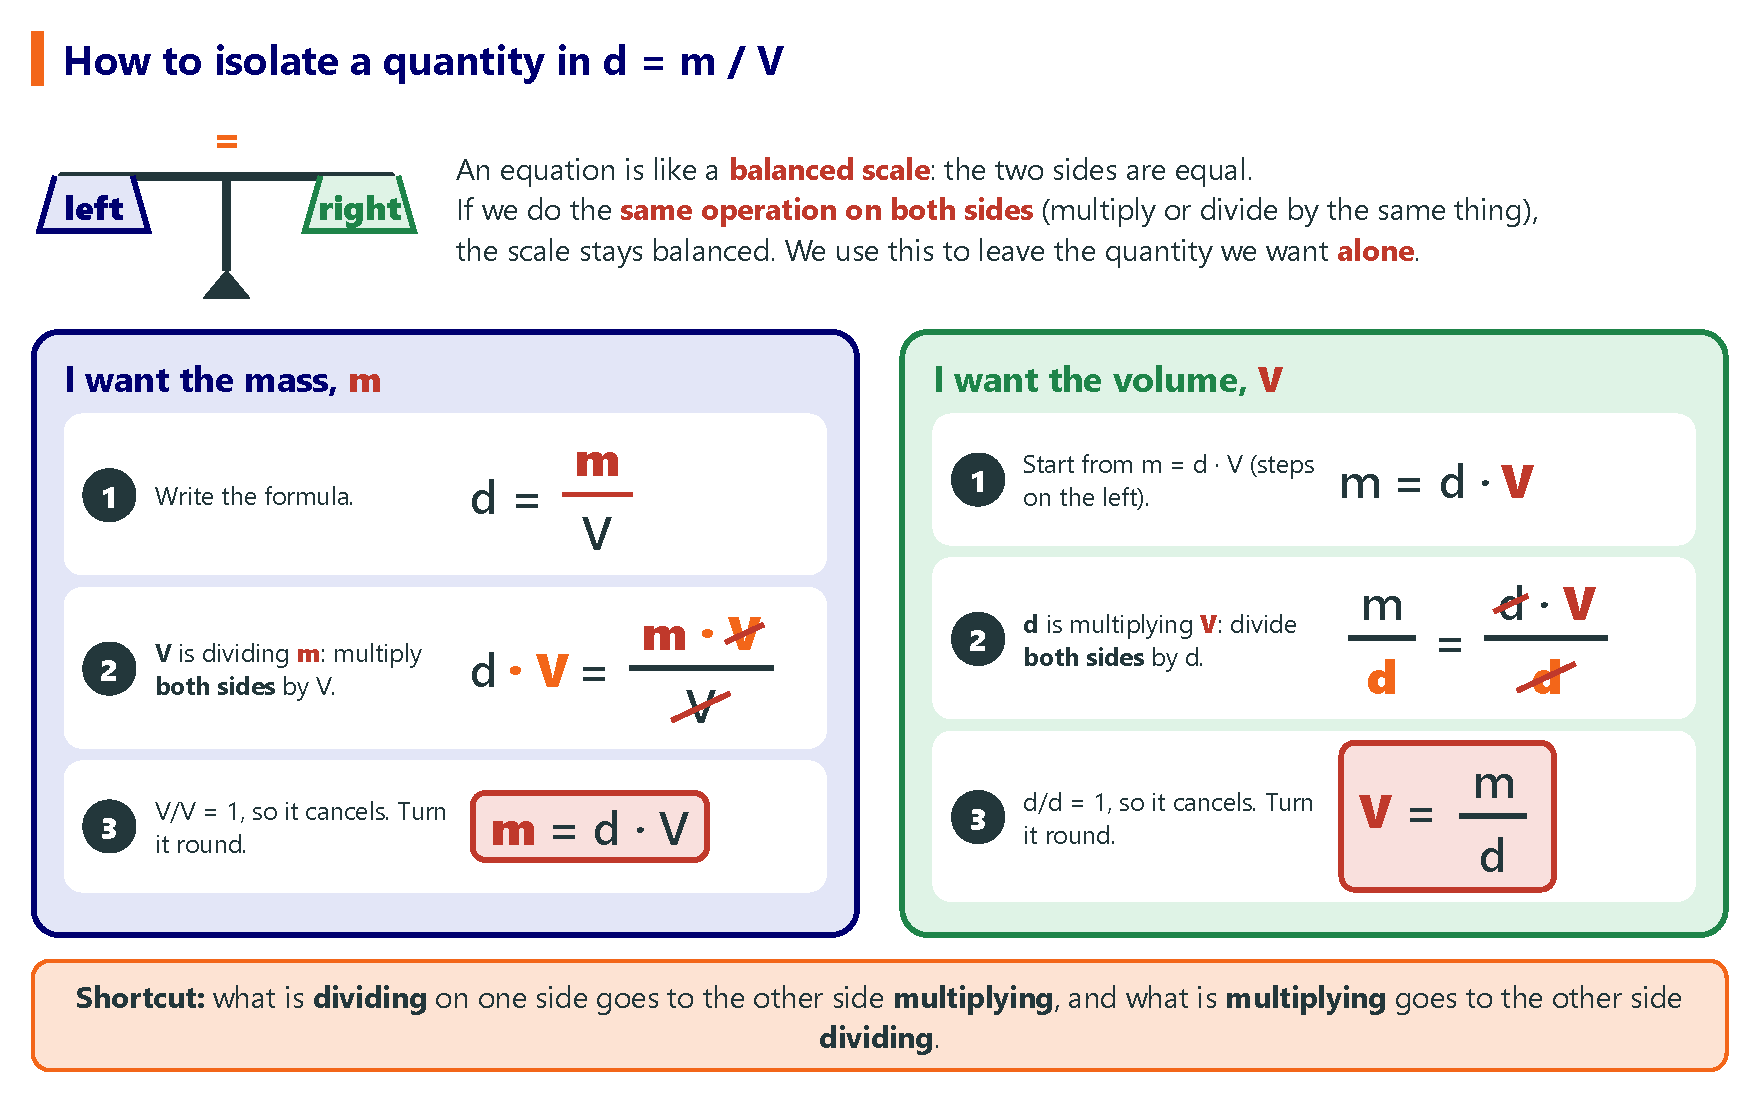
\includegraphics[width=\textwidth]{FigurasSVG/Unit_1_Matter_Measurement/pdf/density_isolate.pdf}
    \caption{Isolating the mass and the volume in the density formula, step by step.}
    \label{fig:u1_density_isolate}
\end{figure}

\negsubro{Method, step by step}:
\begin{enumerate}[label=\numberballmDarkTeal]
    \item Read the exercise and write the \textbf{data} with their units. Underline the quantity that the exercise asks for (the \textbf{unknown}).
    \item Write the formula \(d = \dfrac{m}{V}\).
    \item Look at what is \textbf{next to} the unknown and do the \textbf{opposite operation on both sides}:
    \begin{itemize}
        \item If the unknown is being \textbf{divided} by something, \textbf{multiply} both sides by it.
        \item If the unknown is being \textbf{multiplied} by something, \textbf{divide} both sides by it.
    \end{itemize}
    \item Cancel what is repeated above and below (it is worth 1) and write the unknown on the left: \(m = d \cdot V\) or \(V = \dfrac{m}{d}\).
    \item Substitute the numbers \textbf{with their units}, calculate and check that the unit of the result makes sense.
\end{enumerate}

\begin{impt}
    The three versions of the same formula:
    \begin{equation*}
        d = \dfrac{m}{V} \qquad\qquad m = d \cdot V \qquad\qquad V = \dfrac{m}{d}
    \end{equation*}
    \textbf{Shortcut}: what is \textbf{dividing} on one side goes to the other side \textbf{multiplying}, and what is \textbf{multiplying} goes to the other side \textbf{dividing}.
\end{impt}

\begin{example}
    \textbf{Calculating a mass.} A gold ring has a volume of \qty{0.8}{\cubic\cm}. The density of gold is \qty{19.3}{\g\per\cubic\cm}. What is the mass of the ring?
    \begin{enumerate}[label=\numberballmDarkTeal]
        \item Data: \(V = \qty{0.8}{\cubic\cm}\), \(d = \qty{19.3}{\g\per\cubic\cm}\). Unknown: \(\underline{m}\).
        \item Formula: \(d = \dfrac{m}{V}\).
        \item \(m\) is being divided by \(V\), so we multiply both sides by \(V\):
        \(\;d \cdot V = \dfrac{m \cdot \cancelred{V}}{\cancelred{V}}\)
        \item \(m = d \cdot V\)
        \item \(m = \qty{19.3}{\g\per\cubic\cm} \cdot \qty{0.8}{\cubic\cm} = \textcolor{red}{\qty{15.44}{\g}}\)
    \end{enumerate}
\end{example}

\begin{example}
    \textbf{Calculating a volume.} We want to pour \qty{500}{\g} of olive oil into a jug. The density of olive oil is \qty{0.92}{\g\per\mL}. What volume of oil is that?
    \begin{enumerate}[label=\numberballmDarkTeal]
        \item Data: \(m = \qty{500}{\g}\), \(d = \qty{0.92}{\g\per\mL}\). Unknown: \(\underline{V}\).
        \item Formula: \(d = \dfrac{m}{V}\). First we take \(V\) up (it is dividing, so it goes to the other side multiplying): \(m = d \cdot V\).
        \item \(V\) is being multiplied by \(d\), so we divide both sides by \(d\):
        \(\;\dfrac{m}{d} = \dfrac{\cancelred{d} \cdot V}{\cancelred{d}}\)
        \item \(V = \dfrac{m}{d}\)
        \item \(V = \dfrac{\qty{500}{\g}}{\qty{0.92}{\g\per\mL}} \approx \textcolor{red}{\qty{543}{\mL}}\)
    \end{enumerate}
\end{example}

\begin{exercise}
    Isolate the unknown and calculate:
    \begin{enumerate}[label=\letraminuscula]
        \item The mass of \qty{250}{\mL} of milk (\(d = \qty{1.03}{\g\per\mL}\)).
        \item The volume of \qty{100}{\g} of mercury (\(d = \qty{13.6}{\g\per\mL}\)).
        \item The mass of an ice cube of \qty{30}{\cubic\cm} (\(d = \qty{0.92}{\g\per\cubic\cm}\)).
        \item The volume of an aluminium piece of \qty{54}{\g} (\(d = \qty{2.70}{\g\per\cubic\cm}\)).
    \end{enumerate}
    \begin{solu}
        \begin{enumerate}[label=\alph*)]
            \item \(m = d \cdot V = \qty{1.03}{\g\per\mL} \cdot \qty{250}{\mL} = \qty{257.5}{\g}\)
            \item \(V = \dfrac{m}{d} = \dfrac{\qty{100}{\g}}{\qty{13.6}{\g\per\mL}} \approx \qty{7.35}{\mL}\)
            \item \(m = d \cdot V = \qty{0.92}{\g\per\cubic\cm} \cdot \qty{30}{\cubic\cm} = \qty{27.6}{\g}\)
            \item \(V = \dfrac{m}{d} = \dfrac{\qty{54}{\g}}{\qty{2.70}{\g\per\cubic\cm}} = \qty{20}{\cubic\cm}\)
        \end{enumerate}
    \end{solu}
\end{exercise}

\begin{exercise}
    The same method works with any formula of the type \(a = \dfrac{b}{c}\). The speed of a cyclist is \(v = \dfrac{s}{t}\), where \(s\) is the distance and \(t\) the time.
    \begin{enumerate}[label=\letraminuscula]
        \item Isolate \(s\) and \(t\), explaining the operation you do in each step.
        \item A cyclist rides at \qty{5}{\m\per\s} for \qty{120}{\s}. What distance does she cover?
        \item How long does it take her to cover \qty{1500}{\m} at the same speed?
    \end{enumerate}
    \begin{solu}
        \begin{enumerate}[label=\alph*)]
            \item \(s\) is divided by \(t\): we multiply both sides by \(t\) \(\to\) \(s = v \cdot t\). Then \(t\) is multiplied by \(v\): we divide both sides by \(v\) \(\to\) \(t = \dfrac{s}{v}\).
            \item \(s = v \cdot t = \qty{5}{\m\per\s} \cdot \qty{120}{\s} = \qty{600}{\m}\)
            \item \(t = \dfrac{s}{v} = \dfrac{\qty{1500}{\m}}{\qty{5}{\m\per\s}} = \qty{300}{\s}\)
        \end{enumerate}
    \end{solu}
\end{exercise}

\begin{exercise}
    A glass contains \qty{50}{\cmcubicos} of oil and \qty{120}{\cmcubicos} of water at \qty{20}{\celsius}. Oil is yellow, does not dissolve in water and floats because its density (\qty{0.9}{\g\per\mL}) is lower than that of water (\qty{1.0}{\g\per\mL}).
    \begin{enumerate}[label=\letraminuscula]
        \item List all the properties of matter mentioned in the text.
        \item Classify each property as quantitative/qualitative and as extensive/intensive.
    \end{enumerate}
    \begin{solu}
        \begin{enumerate}[label=\alph*)]
            \item Volume of oil, volume of water, colour of oil, solubility of oil in water, density of oil, density of water, temperature.
            \item Volumes: \textbf{quantitative, extensive}. Temperature: \textbf{quantitative, intensive}. Colour: \textbf{qualitative, intensive}. Solubility and density: \textbf{quantitative, intensive} (characteristic properties).
        \end{enumerate}
    \end{solu}
\end{exercise}

\begin{exercise}
    Match each object with the property most commonly used to choose it: copper wire, steel saucepan, cork stopper, cocoa powder, antifreeze liquid \(\;\to\;\) electrical conductivity, melting point, density, solubility in milk, thermal conductivity.
    \begin{solu}
        Copper wire \(\to\) electrical conductivity. \\
        Steel saucepan \(\to\) thermal conductivity. \\
        Cork stopper \(\to\) density. \\
        Cocoa powder \(\to\) solubility in milk. \\
        Antifreeze liquid \(\to\) melting point.
    \end{solu}
\end{exercise}

\begin{exercise}
    Classify each property as \textbf{general} or \textbf{characteristic}, and explain your reasoning: mass, boiling point, volume, hardness, temperature, density.
    \begin{solu}
        \textbf{General}: mass, volume, temperature (any type of matter can have any value, so they do not identify a substance). \\
        \textbf{Characteristic}: boiling point, hardness, density (each substance has its own value, so they can be used to identify it).
    \end{solu}
\end{exercise}

\begin{exercise}
    Two identical-looking metal cubes have masses of \qty{270}{\g} and \qty{789}{\g}, but both have a volume of \qty{100}{\cubic\cm}.
    \begin{enumerate}[label=\letraminuscula]
        \item Are mass and volume enough to tell us if the two cubes are made of the same metal? Explain.
        \item Calculate the density of each cube. Are they the same metal?
    \end{enumerate}
    \begin{solu}
        \begin{enumerate}[label=\alph*)]
            \item No, because mass and volume are \textbf{general (extensive)} properties: two different substances can have the same mass or the same volume.
            \item \(d_1 = \dfrac{\qty{270}{\g}}{\qty{100}{\mL}} = \qty{2.70}{\g\per\mL}\) (aluminium); \(d_2 = \dfrac{\qty{789}{\g}}{\qty{100}{\mL}} = \qty{7.89}{\g\per\mL}\) (iron). The densities are different, so \textbf{they are not the same metal}.
        \end{enumerate}
    \end{solu}
\end{exercise}

\begin{exercise}
    Write the data, isolate the unknown and calculate:
    \begin{enumerate}[label=\letraminuscula]
        \item A marble has a mass of \qty{5}{\g} and a volume of \qty{2}{\cubic\cm}. Calculate the density of the marble, in \unit{\g\per\cubic\cm}.
        \item A block of wood has a density of \qty{0.75}{\g\per\cubic\cm} and a volume of \qty{120}{\cubic\cm}. Calculate the mass of the block of wood, in grams.
        \item A brick has a density of \qty{500}{\kg\per\cubic\m} and a mass of \qty{10.5}{\kg}. Calculate the volume of the brick, in \unit{\cubic\m}.
        \item A metal rod has a mass of \qty{150}{\g} and a volume of \qty{25}{\cubic\cm}. Calculate the density of the rod, in \unit{\g\per\cubic\cm}.
        \item A piece of aluminium has a density of \qty{2.6}{\g\per\cubic\cm} and a volume of \qty{15}{\cubic\cm}. Calculate the mass of the aluminium, in grams.
        \item A piece of carbon has a density of \qty{2.2}{\g\per\cubic\cm} and a volume of \qty{70}{\cubic\cm}. Calculate the mass of the piece of carbon, in grams.
        \item A cube has a side length of \qty{8}{\cm} and a mass of \qty{960}{\g}. Calculate the density of the cube, in \unit{\g\per\cubic\cm}.
    \end{enumerate}
    \begin{solu}
        \begin{enumerate}[label=\alph*)]
            \item \(d = \dfrac{m}{V} = \dfrac{\qty{5}{\g}}{\qty{2}{\cubic\cm}} = \qty{2.5}{\g\per\cubic\cm}\)
            \item \(m = d \cdot V = \qty{0.75}{\g\per\cubic\cm} \cdot \qty{120}{\cubic\cm} = \qty{90}{\g}\)
            \item \(V = \dfrac{m}{d} = \dfrac{\qty{10.5}{\kg}}{\qty{500}{\kg\per\cubic\m}} = \qty{0.021}{\cubic\m} = \qty{2.1e-2}{\cubic\m}\)
            \item \(d = \dfrac{m}{V} = \dfrac{\qty{150}{\g}}{\qty{25}{\cubic\cm}} = \qty{6}{\g\per\cubic\cm}\)
            \item \(m = d \cdot V = \qty{2.6}{\g\per\cubic\cm} \cdot \qty{15}{\cubic\cm} = \qty{39}{\g}\)
            \item \(m = d \cdot V = \qty{2.2}{\g\per\cubic\cm} \cdot \qty{70}{\cubic\cm} = \qty{154}{\g}\)
            \item First the volume of the cube: \(V = \qty{8}{\cm} \cdot \qty{8}{\cm} \cdot \qty{8}{\cm} = \qty{512}{\cubic\cm}\). \\
            \(d = \dfrac{m}{V} = \dfrac{\qty{960}{\g}}{\qty{512}{\cubic\cm}} \approx \qty{1.88}{\g\per\cubic\cm}\)
        \end{enumerate}
    \end{solu}
\end{exercise}



\begin{figure}[H]
    \centering
    % [FIGURA ORIGINAL] \includegraphics[width=0.95\textwidth]{Unit_1/density_column}
    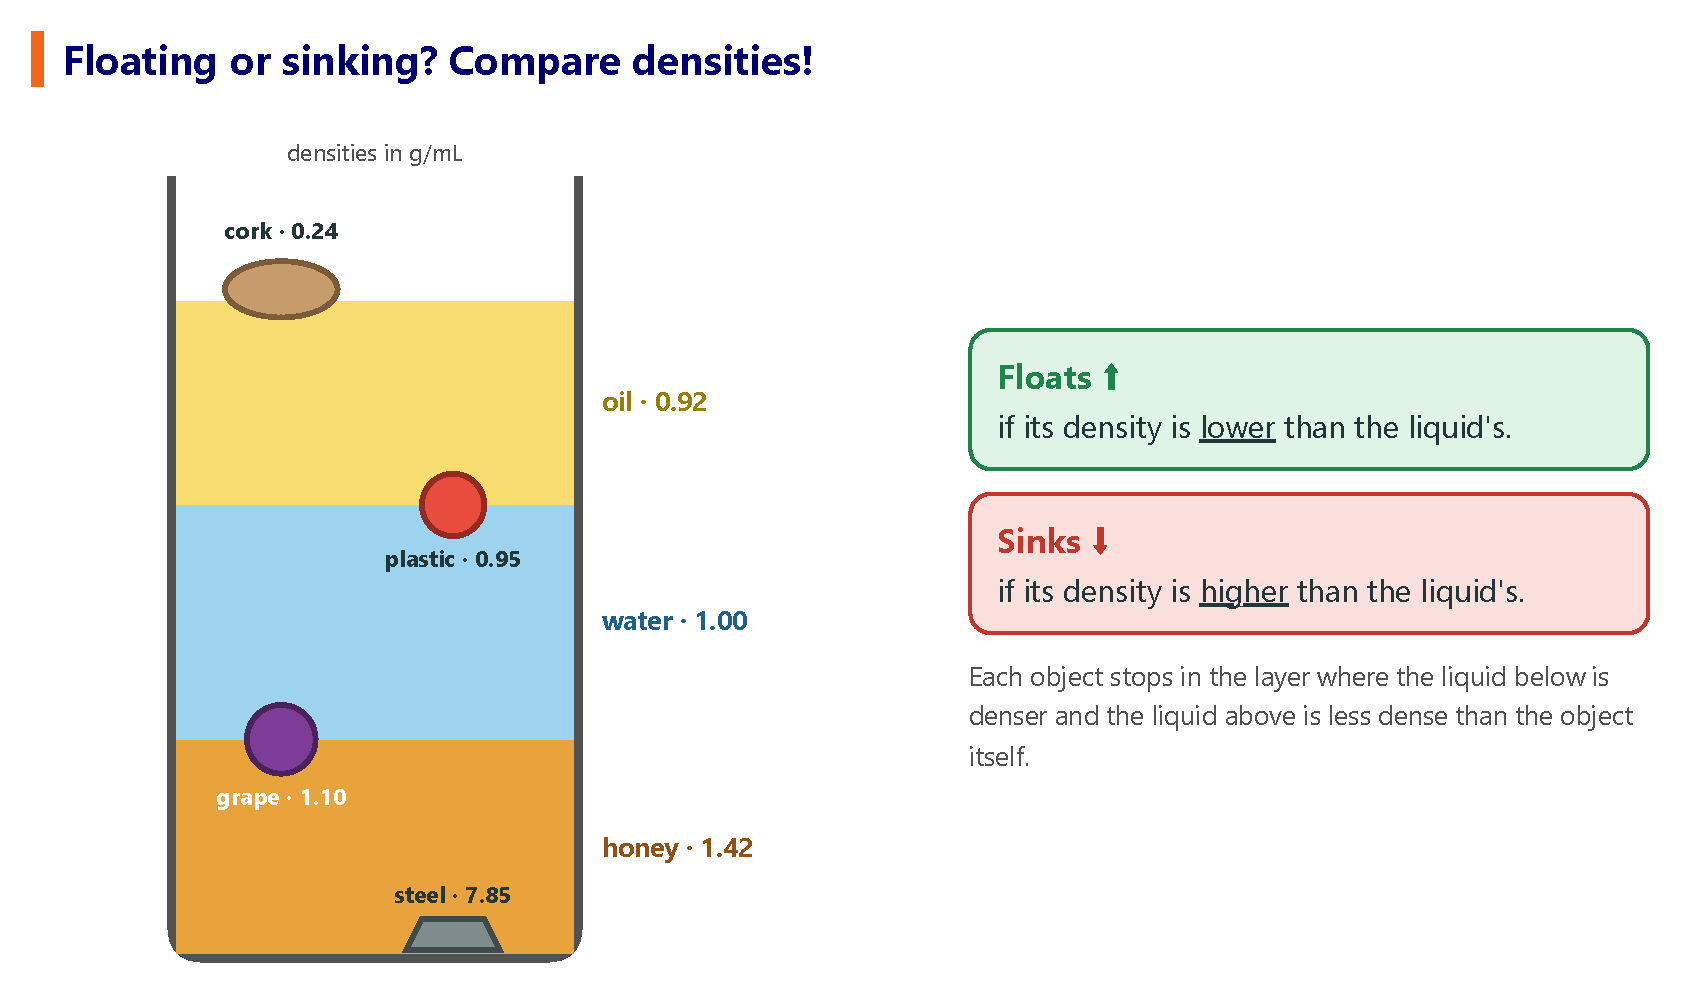
\includegraphics[width=0.95\textwidth]{FigurasSVG/Unit_1_Matter_Measurement/pdf/density_column.pdf}
    \caption{A density column: each object floats or sinks depending on its density.}
    \label{fig:u1_density_column}
\end{figure}

\begin{impt}
    In water (\(d = \qty{1.00}{\g\per\mL}\)):
    \begin{itemize}
        \item \(d_{\text{object}} < \qty{1.00}{\g\per\mL}\) \(\to\) it \textbf{floats}.
        \item \(d_{\text{object}} > \qty{1.00}{\g\per\mL}\) \(\to\) it \textbf{sinks}.
    \end{itemize}
\end{impt}

\begin{didyouknow}
    Ice (\qty{0.92}{\g\per\mL}) is less dense than liquid water, so icebergs float\ldots{} but about \textbf{90\,\%} of an iceberg is hidden under the surface. That is where the expression ``the tip of the iceberg'' comes from!
\end{didyouknow}

\begin{exercise}
    The densities of cork, aluminium and glycerin are \qty{0.24}{\g\per\mL}, \qty{2.70}{\g\per\mL} and \qty{1.26}{\g\per\mL}, respectively.
    \begin{enumerate}[label=\letraminuscula]
        \item Which of them float in water (\(d = \qty{1.00}{\g\per\mL}\))?
        \item Mercury has a density of \qty{13.6}{\g\per\mL}. Which of the three materials would float on mercury?
    \end{enumerate}
    \begin{solu}
        \begin{enumerate}[label=\alph*)]
            \item Cork floats in water (\(0.24 < 1.00\)). Aluminium and glycerin sink (\(2.70 > 1.00\) and \(1.26 > 1.00\)).
            \item All three have a density lower than mercury's, so \textbf{cork, aluminium and glycerin would all float on mercury}.
        \end{enumerate}
    \end{solu}
\end{exercise}

\begin{exercise}
    A wooden block has a mass of \qty{45}{\g} and a volume of \qty{60}{\cubic\cm}.
    \begin{enumerate}[label=\letraminuscula]
        \item Calculate its density.
        \item Will it float or sink in water? Justify your answer.
    \end{enumerate}
    \begin{solu}
        \begin{enumerate}[label=\alph*)]
            \item \(d = \dfrac{m}{V} = \dfrac{\qty{45}{\g}}{\qty{60}{\cubic\cm}} = \qty{0.75}{\g\per\cubic\cm}\).
            \item Since \(\qty{0.75}{\g\per\mL} < \qty{1.00}{\g\per\mL}\) (water), the block \textbf{floats}.
        \end{enumerate}
    \end{solu}
\end{exercise}

\begin{exercise}
    A ship is made of steel, which has a density of about \qty{7.85}{\g\per\mL}, much higher than water's. Explain, using the idea of density, why a solid steel block sinks but a steel ship floats.
    \begin{solu}
        A ship is mostly hollow (full of air), so its total volume is much larger than that of a solid steel block of the same mass. This makes the \textbf{average density of the whole ship} lower than that of water, so it floats, even though steel itself is denser than water.
    \end{solu}
\end{exercise}


%----------------------------------------------------------------------------------------

\section{Measuring instruments}

\subsection{Measuring mass}

\begin{figure}[H]
    \centering
    % [FIGURA ORIGINAL] \includegraphics[width=\textwidth]{Unit_1/balances}
    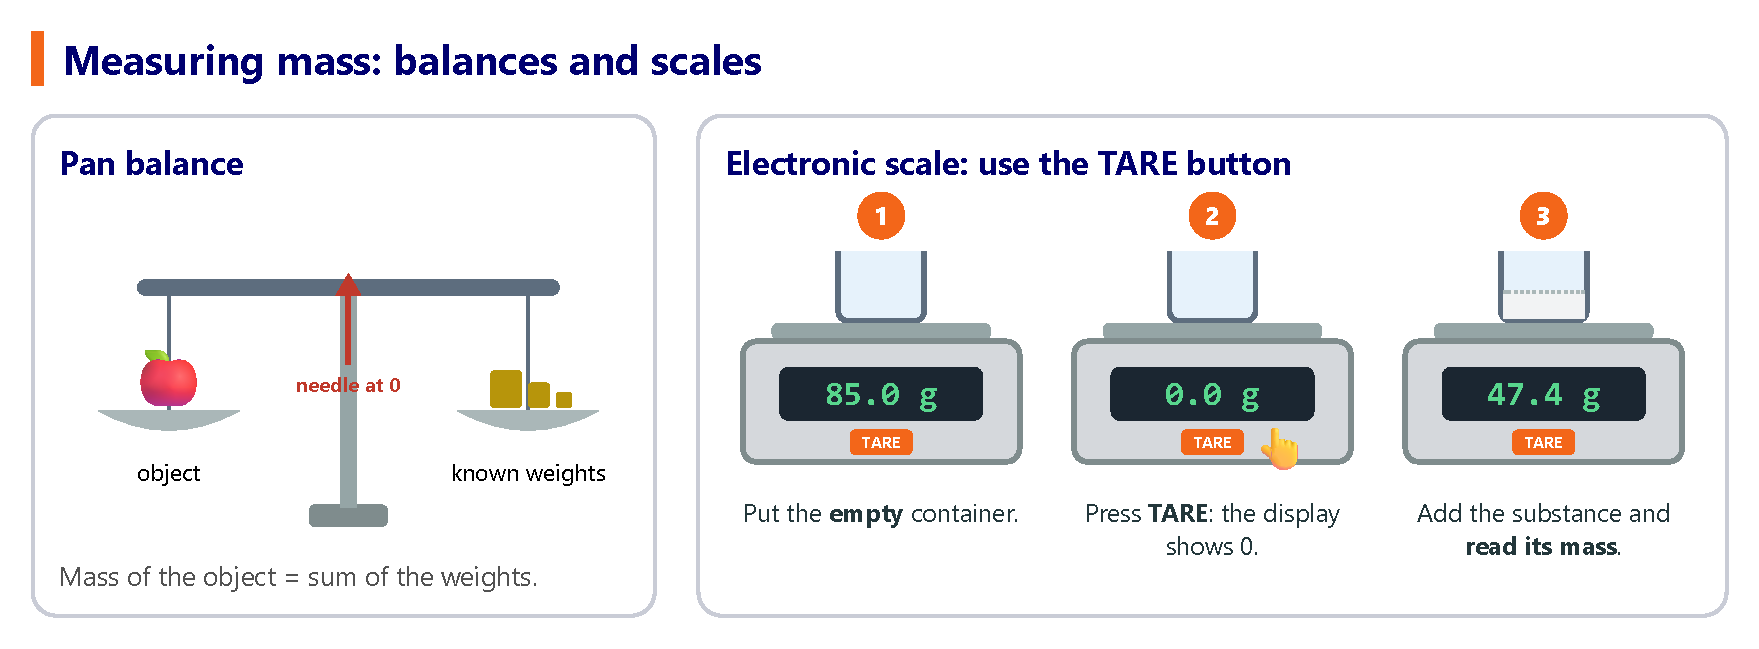
\includegraphics[width=\textwidth]{FigurasSVG/Unit_1_Matter_Measurement/pdf/balances.pdf}
    \caption{A pan balance and an electronic scale with its TARE button.}
    \label{fig:u1_balances}
\end{figure}

\begin{itemize}
    \item \negsubro{Pan balance}: put the object on one pan and add known weights to the other until the needle points to 0. Mass of the object = sum of the weights.
    \item \negsubro{Electronic scale}: put the empty container, press \textbf{TARE} (the display shows 0) and add the substance. The display shows only the mass of the substance.
\end{itemize}

\begin{impt}
    \negsubro{Mass is not weight}. \textbf{Mass} is the amount of matter (\unit{\kg}) and it is the same everywhere. \textbf{Weight} is the force with which a planet pulls a body (\unit{\N}): on the Moon you would weigh six times less, but your mass would not change.
\end{impt}

\begin{exercise}
    Explain why we press ``tare'' before adding a substance to an electronic scale, instead of simply weighing the container with the substance inside and subtracting by hand.
    \begin{solu}
        Pressing ``tare'' resets the display to zero with the empty container already on the scale, so the mass shown afterwards is directly the mass of the substance alone. This saves time and prevents calculation mistakes.
    \end{solu}
\end{exercise}

\begin{exercise}
    A student places an empty beaker on an electronic scale without pressing tare: it reads \qty{85.0}{\g}. They then add some salt, and the scale now reads \qty{132.4}{\g}.
    \begin{enumerate}[label=\letraminuscula]
        \item Calculate the mass of the salt.
        \item Explain how using ``tare'' would have made this measurement more direct.
    \end{enumerate}
    \begin{solu}
        \begin{enumerate}[label=\alph*)]
            \item Mass of salt \(= \qty{132.4}{\g} - \qty{85.0}{\g} = \qty{47.4}{\g}\).
            \item With tare, the scale would have read \qty{0}{\g} with the empty beaker, so the final reading would have been directly \qty{47.4}{\g}.
        \end{enumerate}
    \end{solu}
\end{exercise}

\subsection{Measuring volume}

\begin{itemize}
    \item \negsubro{Regular bodies} (cube, prism, cylinder, sphere\ldots): we measure their lengths and use a formula.
    \item \negsubro{Liquids and irregular bodies}: we use a \textbf{graduated cylinder}, a \textbf{burette} or a \textbf{pipette}.
\end{itemize}

\begin{definition}[Meniscus]
    The curved surface of a liquid inside a narrow tube. We read the volume at the \textbf{bottom} of the meniscus, with our eyes at the same height as the liquid.
\end{definition}

\begin{figure}[H]
    \centering
    % [FIGURA ORIGINAL] \includegraphics[width=\textwidth]{Unit_1/meniscus}
    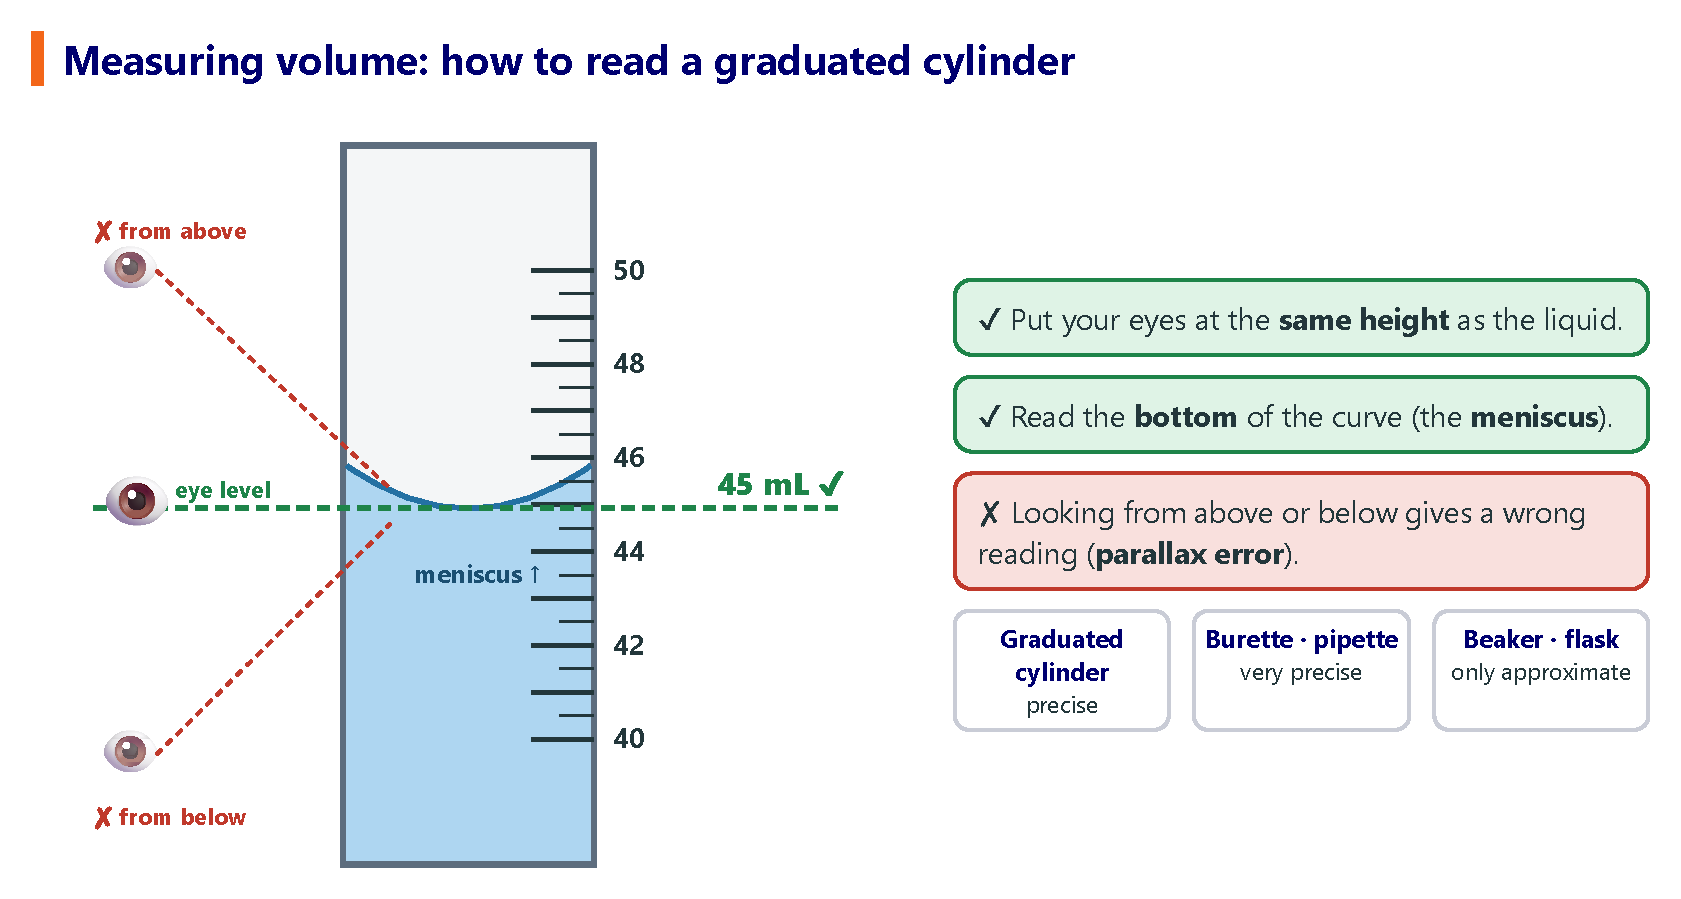
\includegraphics[width=\textwidth]{FigurasSVG/Unit_1_Matter_Measurement/pdf/meniscus.pdf}
    \caption{The correct way to read a graduated cylinder.}
    \label{fig:u1_meniscus}
\end{figure}

\begin{exercise}
    A \qty{25}{\mL} graduated cylinder allows \qty{0.5}{\mL} to be measured, and a \qty{250}{\mL} one allows \qty{5}{\mL} to be measured. Which of the two gives a more precise measurement? Why would you choose the smaller one to measure \qty{18}{\mL} of a liquid?
    \begin{solu}
        The \qty{25}{\mL} cylinder is more precise, because its smallest division (\qty{0.5}{\mL}) is smaller. \\
        For \qty{18}{\mL}, the \qty{25}{\mL} cylinder is the right choice: the liquid fills most of the cylinder and the reading is more precise.
    \end{solu}
\end{exercise}

\begin{exercise}
    Say which instrument (regular-body formula, graduated cylinder, or Erlenmeyer flask) you would use to measure the volume of each of the following, and explain why:
    \begin{enumerate}[label=\letraminuscula]
        \item A wooden cube of \qty{4}{\cm} side.
        \item \qty{35}{\mL} of vinegar for a recipe.
        \item A small, irregularly shaped stone.
        \item Roughly how much water is left in a bottle.
    \end{enumerate}
    \begin{solu}
        \begin{enumerate}[label=\alph*)]
            \item A regular body: measure the side with a ruler and use \(V = \text{side}^3\).
            \item A graduated cylinder, because it gives a precise reading of a liquid's volume.
            \item A graduated cylinder, using the rise in the water level, since the stone is irregular.
            \item An Erlenmeyer flask or beaker, since only an approximate volume is needed.
        \end{enumerate}
    \end{solu}
\end{exercise}

\begin{exercise}
    When reading the volume of water in a graduated cylinder, why must we place our eyes at the same height as the liquid's surface, and why do we read the \textbf{bottom} of the meniscus and not the top?
    \begin{solu}
        If we look from above or below, the reading is too high or too low (\textbf{parallax error}). Looking at eye level avoids this error. \\
        We read the bottom of the meniscus because water sticks to the glass walls and rises slightly at the edges; the bottom of the curve is the point that truly corresponds to the volume of liquid.
    \end{solu}
\end{exercise}

%\subsection{Precision of an instrument}
%
%\begin{definition}[Sensitivity (or appreciation) of an instrument]
%    The smallest amount that an instrument can measure: the value of its \textbf{smallest division}.
%\end{definition}
%
%\begin{figure}[H]
%    \centering
%    \includegraphics[width=\textwidth]{Unit_1/sensitivity_rulers}
%    \caption{The smaller the sensitivity, the more precise the measurement.}
%    \label{fig:u1_sensitivity_rulers}
%\end{figure}
%
%\begin{definition}[Precision and accuracy]
%    A measurement is \textbf{precise} when repeating it gives very similar values, and \textbf{accurate} when it is close to the real value. A badly calibrated instrument can be precise but not accurate.
%\end{definition}
%
%\begin{figure}[H]
%    \centering
%    \includegraphics[width=\textwidth]{Unit_1/precision_accuracy}
%    \caption{Precision and accuracy explained with a target.}
%    \label{fig:u1_precision_accuracy}
%\end{figure}
%
%\begin{exercise}
%    Three electronic scales show these masses for the same coin: scale A gives \qty{2.5}{\g}, scale B gives \qty{2.52}{\g} and scale C gives \qty{2.524}{\g}.
%    \begin{enumerate}[label=\letraminuscula]
%        \item Order the three scales from least to most precise.
%        \item If the coin's real mass is known to be \qty{2.50}{\g}, which of the three measurements is the most accurate?
%    \end{enumerate}
%    \begin{solu}
%        \begin{enumerate}[label=\alph*)]
%            \item From least to most precise: A (sensitivity \qty{0.1}{\g}) \(<\) B (\qty{0.01}{\g}) \(<\) C (\qty{0.001}{\g}).
%            \item Scale A's reading (\qty{2.5}{\g}) is exactly the real value, so it is the most \textbf{accurate}, even though it is the least precise.
%        \end{enumerate}
%    \end{solu}
%\end{exercise}
%
%\begin{exercise}
%    A ruler has millimetre divisions, and a tape measure used in a workshop has only centimetre divisions.
%    \begin{enumerate}[label=\letraminuscula]
%        \item What is the sensitivity of each instrument?
%        \item Which one would you use to measure the length of a pencil as precisely as possible? Explain.
%    \end{enumerate}
%    \begin{solu}
%        \begin{enumerate}[label=\alph*)]
%            \item Ruler: \qty{1}{\mm}. Tape measure: \qty{1}{\cm}.
%            \item The \textbf{ruler}, because its sensitivity is smaller (\(\qty{1}{\mm} < \qty{1}{\cm}\)), so it allows a more precise reading.
%        \end{enumerate}
%    \end{solu}
%\end{exercise}
%
%\begin{exercise}
%    Four archers shoot four arrows each at a target. Archer 1's arrows all land close together, but far from the bullseye. Archer 2's arrows land scattered all around the target. Archer 3's arrows all land close together, right on the bullseye. Archer 4's arrows land scattered but roughly centred on the bullseye.
%    \begin{enumerate}[label=\letraminuscula]
%        \item Which archer represents ``precise but not accurate''?
%        \item Which archer represents ``precise and accurate''?
%    \end{enumerate}
%    \begin{solu}
%        \begin{enumerate}[label=\alph*)]
%            \item Archer 1: the arrows are close together (precise) but far from the bullseye (not accurate).
%            \item Archer 3: the arrows are close together (precise) and on the bullseye (accurate).
%        \end{enumerate}
%    \end{solu}
%\end{exercise}

%----------------------------------------------------------------------------------------

\section{Indirect measurements}

\begin{definition}[Indirect measurement]
    A measurement that we \textbf{calculate} from other quantities that we have measured directly.
\end{definition}

Mass and length can be read directly on an instrument, but surface area, density or very small thicknesses usually have to be \textbf{calculated}.

%\subsection{Measuring surface area indirectly}
%
%\begin{figure}[H]
%    \centering
%    \includegraphics[width=\textwidth]{Unit_1/indirect_area}
%    \caption{The surface of an irregular shape is proportional to its mass if the material is the same.}
%    \label{fig:u1_indirect_area}
%\end{figure}
%
%\vspace{2.5\baselineskip}
%% centered by hand: with fleqn an equation* goes to the left margin and the left labels fall off the page
%\begin{center}
%    \(\displaystyle
%        \eqnmarkbox[ochre]{u1sf}{S_F} =
%        \eqnmarkbox[signBlue]{u1sm}{S_M} \cdot
%        \dfrac{\eqnmarkbox[indigo2]{u1mf}{M_F}}{\eqnmarkbox[firebrick]{u1mm}{M_M}}
%    \)
%\end{center}
%\annotate[yshift=1.2em]{above,left}{u1sf}{Surface of the irregular figure}
%\annotate[yshift=-1.2em]{below,left}{u1sm}{Surface of the measured square}
%\annotate[yshift=1.2em]{above,right}{u1mf}{Mass of the cut-out figure}
%\annotate[yshift=-1.2em]{below,right}{u1mm}{Mass of the measured square}
%\vspace{2.5\baselineskip}
%
%\begin{exercise}
%    To find the surface area of an irregularly shaped leaf, a student cuts a square of paper of \(S_M = \qty{1}{\square\dm}\) from the same type of paper and weighs it: \(M_M = \qty{15.0}{\g}\). She then traces the leaf's outline on the same paper, cuts it out and weighs it: \(M_F = \qty{3.0}{\g}\).
%    \begin{enumerate}[label=\letraminuscula]
%        \item Calculate the surface area of the leaf.
%        \item Explain why the measured square and the leaf cut-out must be made of exactly the same paper.
%    \end{enumerate}
%    \begin{solu}
%        \begin{enumerate}[label=\alph*)]
%            \item \(S_F = S_M \cdot \dfrac{M_F}{M_M} = \qty{1}{\square\dm} \cdot \dfrac{\qty{3.0}{\g}}{\qty{15.0}{\g}} = \qty{0.20}{\square\dm}\).
%            \item The method only works if mass is proportional to surface area, which is true only if the paper has the same thickness and density everywhere.
%        \end{enumerate}
%    \end{solu}
%\end{exercise}
%
%\begin{exercise}
%    A measured square of cardboard with \(S_M = \qty{1}{\square\dm}\) has a mass of \(M_M = \qty{40}{\g}\). An irregular piece of the same cardboard has a surface area of \qty{0.65}{\square\dm}. What mass should this irregular piece have?
%    \begin{solu}
%        \(M_F = M_M \cdot \dfrac{S_F}{S_M} = \qty{40}{\g} \cdot \dfrac{\qty{0.65}{\square\dm}}{\qty{1}{\square\dm}} = \qty{26}{\g}\).
%    \end{solu}
%\end{exercise}

\subsection{Measuring density}

\begin{itemize}
    \item \negsubro{Liquid}: tare a graduated cylinder on the scale, pour in the liquid, read its volume \(V\) and its mass \(m\), and calculate \(d = m/V\).
    \item \negsubro{Solid that does not dissolve in water}: weigh it, and find its volume by \textbf{water displacement}, as shown in the figure.
\end{itemize}

\begin{figure}[H]
    \centering
    % [FIGURA ORIGINAL] \includegraphics[width=\textwidth]{Unit_1/density_lab}
    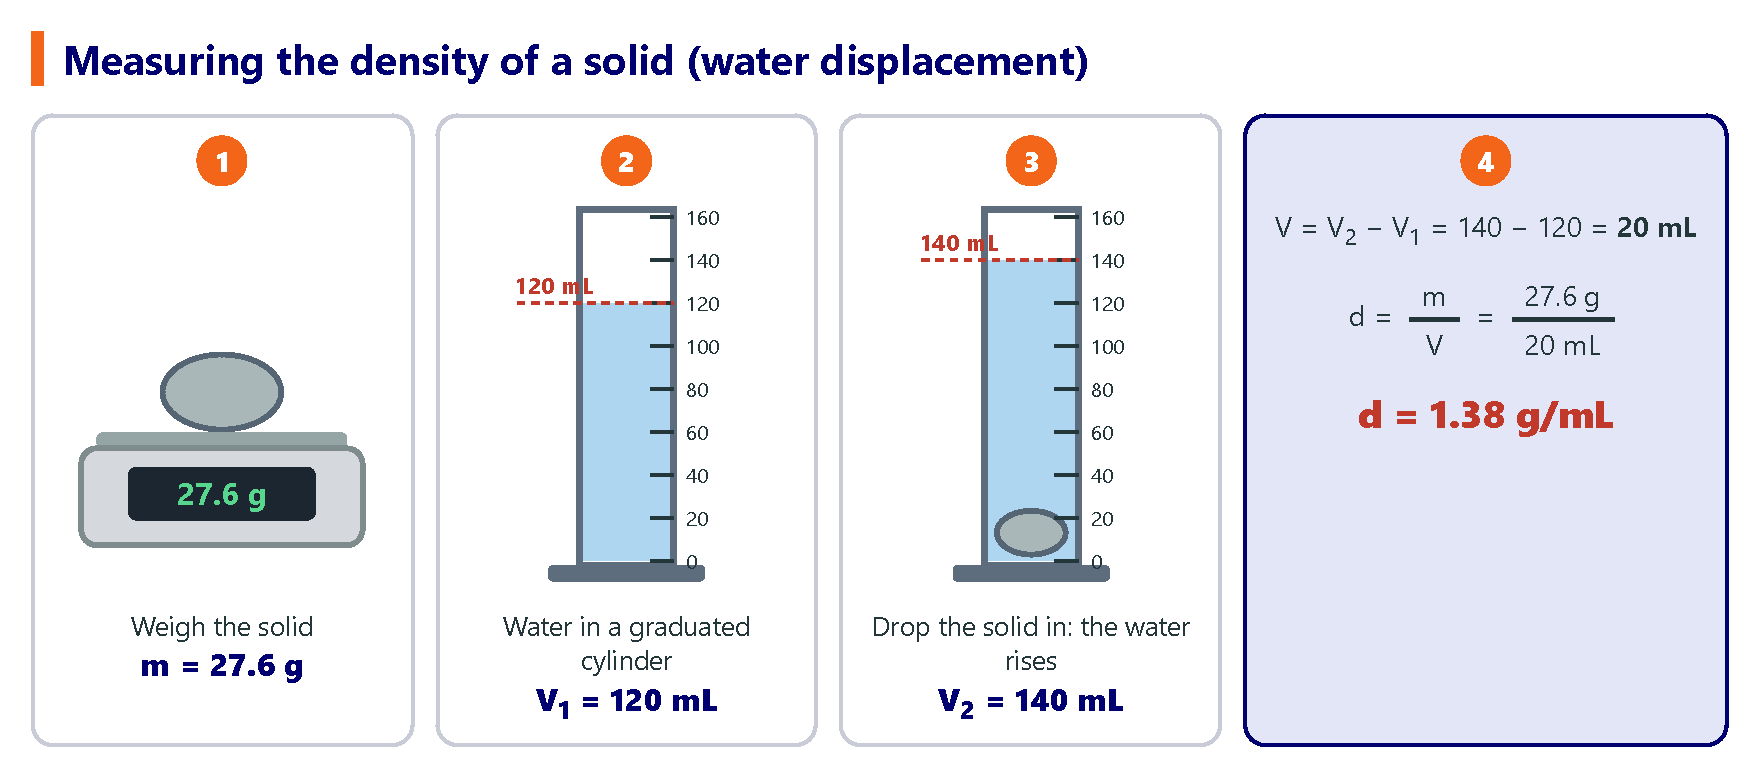
\includegraphics[width=\textwidth]{FigurasSVG/Unit_1_Matter_Measurement/pdf/density_lab.pdf}
    \caption{Measuring the density of a solid: the volume of the solid is the rise in the water level.}
    \label{fig:u1_density_lab}
\end{figure}

\begin{didyouknow}
    According to legend, Archimedes discovered this method in his bath: when he got in, the water level rose. He realised he could use it to measure the volume of the king's crown and check whether it was made of pure gold. He was so excited that he ran into the street shouting ``Eureka!'' (``I have found it!'').
\end{didyouknow}

\begin{exercise}
    A block of modelling clay has a mass of \qty{27.6}{\g}. When we put it into a graduated cylinder with \qty{120}{\mL} of water, the level rises to \qty{140}{\mL}.
    \begin{enumerate}[label=\letraminuscula]
        \item Calculate the density of the modelling clay.
        \item If a second block, made of the same clay, had half the volume, what would its mass and density be?
    \end{enumerate}
    \begin{solu}
        \begin{enumerate}[label=\alph*)]
            \item \(V = \qty{140}{\mL} - \qty{120}{\mL} = \qty{20}{\mL}\); \(d = \dfrac{\qty{27.6}{\g}}{\qty{20}{\mL}} = \qty{1.38}{\g\per\mL}\).
            \item Half the volume (\qty{10}{\mL}) means half the mass (\qty{13.8}{\g}). The \textbf{density does not change} (\qty{1.38}{\g\per\mL}), because it is a characteristic property.
        \end{enumerate}
    \end{solu}
\end{exercise}

\begin{exercise}
    To measure the density of sugar: mass of the empty graduated cylinder = \qty{130}{\g}; mass of the graduated cylinder containing the sugar = \qty{198.5}{\g}; when the sugar is poured into a cylinder with \qty{100}{\mL} of a liquid in which it does not dissolve, the level rises to \qty{130}{\mL}. What is the density of the sugar?
    \begin{solu}
        Mass of sugar \(= \qty{198.5}{\g} - \qty{130}{\g} = \qty{68.5}{\g}\). \\
        Volume of sugar \(= \qty{130}{\mL} - \qty{100}{\mL} = \qty{30}{\mL}\). \\
        Density: \(d = \dfrac{\qty{68.5}{\g}}{\qty{30}{\mL}} \approx \qty{2.28}{\g\per\mL}\).
    \end{solu}
\end{exercise}

\begin{exercise}
    The densities of milk, water and oil are \qty{1.04}{\g\per\mL}, \qty{1.00}{\g\per\mL} and \qty{0.92}{\g\per\mL}, respectively. Calculate the mass of \qty{1}{\litre} of each one.
    \begin{solu}
        Using \(m = d \cdot V\) with \(V = \qty{1000}{\mL}\): \\
        Milk: \(m = \qty{1.04}{\g\per\mL} \cdot \qty{1000}{\mL} = \qty{1040}{\g}\). \\
        Water: \(m = \qty{1000}{\g}\). \\
        Oil: \(m = \qty{920}{\g}\).
    \end{solu}
\end{exercise}

%\subsection{Measuring very small thicknesses indirectly}
%
%Some lengths are too small for a ruler, such as the thickness of a sheet of paper. The trick: measure \textbf{many} of them together and divide.
%
%\begin{figure}[H]
%    \centering
%    \includegraphics[width=\textwidth]{Unit_1/stack_thickness}
%    \caption{The thickness of one sheet is the thickness of the pile divided by the number of sheets.}
%    \label{fig:u1_stack_thickness}
%\end{figure}
%
%\begin{exercise}
%    A pile of 40 identical CD cases is \qty{36}{\cm} tall. Calculate the thickness of a single CD case, in mm.
%    \begin{solu}
%        \(e = \dfrac{\qty{36}{\cm}}{40} = \qty{0.9}{\cm} = \qty{9}{\mm}\).
%    \end{solu}
%\end{exercise}
%
%\begin{exercise}
%    A ream of 500 sheets of paper is \qty{5.5}{\cm} thick.
%    \begin{enumerate}[label=\letraminuscula]
%        \item Calculate the thickness of one sheet, in mm.
%        \item How many sheets would you need to stack to get a pile exactly \qty{1}{\cm} tall?
%    \end{enumerate}
%    \begin{solu}
%        \begin{enumerate}[label=\alph*)]
%            \item \(e = \dfrac{\qty{5.5}{\cm}}{500} = \qty{0.011}{\cm} = \qty{0.11}{\mm}\).
%            \item Number of sheets \(= \dfrac{\qty{1}{\cm}}{\qty{0.011}{\cm}} \approx 91\) sheets.
%        \end{enumerate}
%    \end{solu}
%\end{exercise}
%
%\begin{exercise}
%    Explain why we cannot measure the thickness of a single coin directly and precisely with a ruler that has millimetre divisions, and describe briefly how the indirect method solves this problem.
%    \begin{solu}
%        A coin's thickness (1--2 mm) is very close to the ruler's sensitivity (\qty{1}{\mm}), so a direct reading would have a very large error. \\
%        Stacking many coins gives a much longer length, where the error of the ruler is small in comparison. Dividing by the number of coins gives a much more precise value for one coin.
%    \end{solu}
%\end{exercise}

%----------------------------------------------------------------------------------------

\section{Laboratory equipment and safety rules}

The laboratory is where we do experiments. It is great fun\ldots{} but only if we know the material and follow the safety rules.

\subsection{Common laboratory equipment}

\begin{figure}[H]
    \centering
    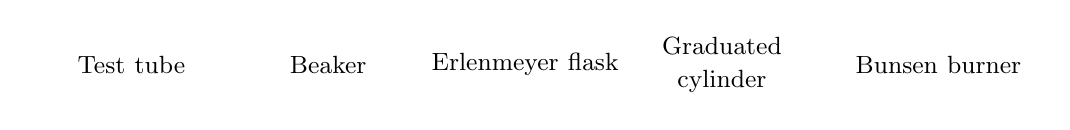
\begin{tikzpicture}[scale=0.5]
        \begin{scope}
            \tkzTestTube[glassType=tube,liquidLevel1=40]
            \node[align=center, text width=2.4cm] at (0,-1) {\small Test tube};
        \end{scope}
        \begin{scope}[xshift=5cm]
            \tkzTestTube[glassType=beaker,liquidLevel1=40]
            \node[align=center, text width=2.4cm] at (0,-1) {\small Beaker};
        \end{scope}
        \begin{scope}[xshift=10cm]
            \tkzTestTube[glassType=erlenmeyer,liquidLevel1=30]
            \node[align=center, text width=2.4cm] at (0,-1) {\small Erlenmeyer flask};
        \end{scope}
        \begin{scope}[xshift=15cm]
            \tkzGraduatedCylinder[liquidLevel1=60]
            \node[align=center, text width=2.4cm] at (0,-1) {\small Graduated cylinder};
        \end{scope}
        \begin{scope}[xshift=20.5cm]
            \tkzBunsenBurner
            \node[align=center, text width=2.4cm] at (0,-1) {\small Bunsen burner};
        \end{scope}
    \end{tikzpicture}
    \caption{Common laboratory glassware and a Bunsen burner, drawn with the \texttt{tikz-chemlab} package.}
    \label{fig:glassware}
\end{figure}

\begin{table}[H]
    \centering
    \small
    \renewcommand{\arraystretch}{1.35}
    \begin{tabular}{p{3.3cm}p{9.5cm}}
        \toprule
        \textbf{Material} & \textbf{What we use it for} \\
        \midrule
        Test tube & hold, heat or mix \textbf{small} amounts of substances \\
        Beaker & mix or heat liquids; measure \textbf{approximate} volumes \\
        Erlenmeyer flask & mix or heat liquids without spilling them (narrow neck) \\
        Graduated cylinder & measure the volume of a liquid \textbf{precisely} \\
        Bunsen burner & heat source (gas flame) \\
        \bottomrule
    \end{tabular}
    \caption{Basic laboratory material and its uses.}
    \label{tab:u1_lab_material}
\end{table}

\subsection{Safety in the laboratory}

\begin{figure}[H]
    \centering
    % [FIGURA ORIGINAL] \includegraphics[width=\textwidth]{Unit_1/lab_safety}
    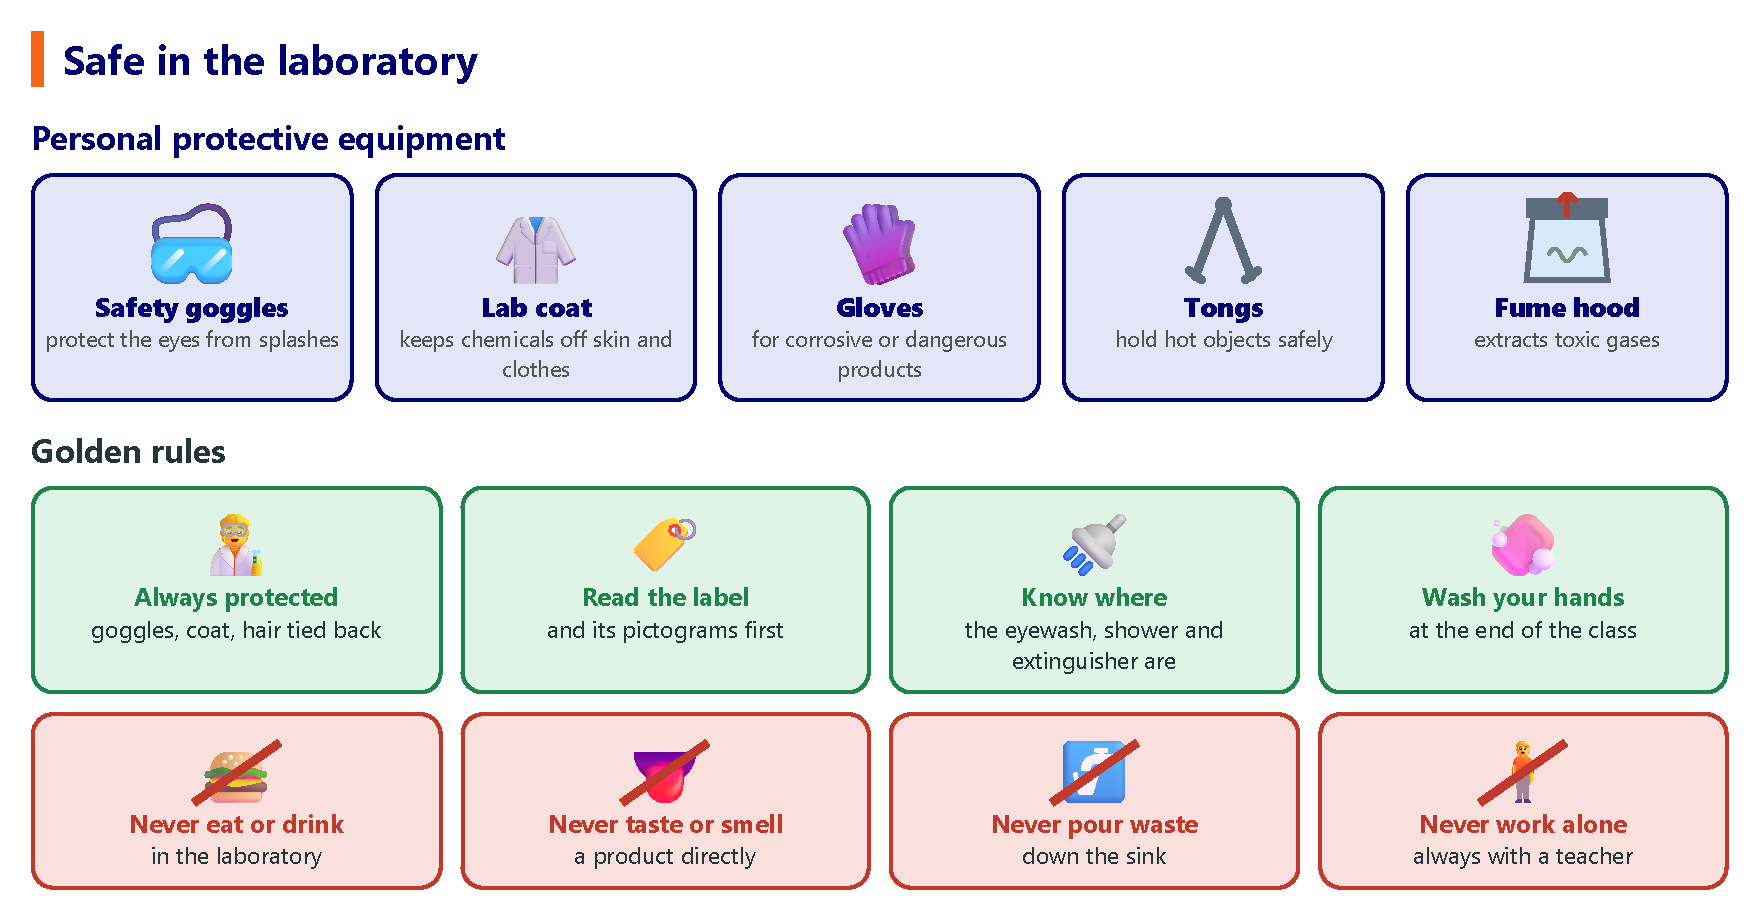
\includegraphics[width=\textwidth]{FigurasSVG/Unit_1_Matter_Measurement/pdf/lab_safety.pdf}
    \caption{Personal protective equipment and golden rules of the laboratory.}
    \label{fig:u1_lab_safety}
\end{figure}

Two more rules that are easy to forget:
\begin{enumerate}[label=\numberballmDarkTeal]
    \item Point a test tube that is being heated \textbf{away} from yourself and from other people.
    \item Keep your bench tidy, and use only the material and amounts that your teacher tells you.
\end{enumerate}

\subsection{Hazard pictograms (GHS)}

\begin{definition}[Hazard pictogram]
    A standardised symbol, black on a white background inside a red diamond, printed on the label of a chemical product to warn us, at a glance, about the type of danger it presents. The current set is fixed by the \negsubro{Globally Harmonized System (GHS)}, used all around the world.
\end{definition}

\begin{figure}[H]
    \centering
    \begin{tabular}{@{}p{5.0cm}p{5.0cm}p{5.0cm}@{}}
        \begin{minipage}{5.0cm}
            \centering
            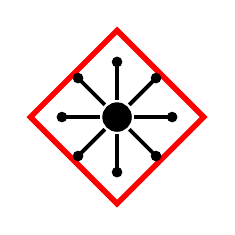
\begin{tikzpicture}
                \draw[draw=red, line width=2pt, fill=white] (0,-1.1) -- (1.1,0) -- (0,1.1) -- (-1.1,0) -- cycle;
                \filldraw[black] (0,0) circle (0.18);
                \foreach \a in {0,45,90,135,180,225,270,315}{
                    \draw[line width=1.4pt] (\a:0.22) -- (\a:0.65);
                    \filldraw[black] (\a:0.7) circle (0.06);
                }
            \end{tikzpicture}\\[2pt]
            \textbf{Explosive}\\[2pt]
            {\small Can explode with heat, shock or friction. Example: fireworks.}
        \end{minipage}
        &
        \begin{minipage}{5.0cm}
            \centering
            
\begin{tikzpicture}
                \draw[draw=red, line width=2pt, fill=white] (0,-1.1) -- (1.1,0) -- (0,1.1) -- (-1.1,0) -- cycle;
                \fill[black] plot [smooth cycle] coordinates {(0,-0.75) (0.32,-0.35) (0.22,0.05) (0.42,0.35) (0.12,0.75) (-0.15,0.35) (-0.32,0.0) (-0.18,-0.35)};
                \fill[white] plot [smooth cycle] coordinates {(0,-0.4) (0.14,-0.1) (0.05,0.15) (0.14,0.35) (0,0.55) (-0.1,0.3) (-0.14,0.0) (-0.05,-0.2)};
            \end{tikzpicture}\\[2pt]
            \textbf{Flammable}\\[2pt]
            {\small Catches fire easily. Example: alcohol, petrol.}
        \end{minipage}
        &
        \begin{minipage}{5.0cm}
            \centering
            
\begin{tikzpicture}
                \draw[draw=red, line width=2pt, fill=white] (0,-1.1) -- (1.1,0) -- (0,1.1) -- (-1.1,0) -- cycle;
                \draw[line width=1.6pt] (0,-0.85) circle (0.2);
                \begin{scope}[yshift=0.15cm]
                    \fill[black] plot [smooth cycle] coordinates {(0,-0.75) (0.32,-0.35) (0.22,0.05) (0.42,0.35) (0.12,0.75) (-0.15,0.35) (-0.32,0.0) (-0.18,-0.35)};
                \end{scope}
            \end{tikzpicture}\\[2pt]
            \textbf{Oxidizing}\\[2pt]
            {\small Feeds a fire, making it burn more strongly. Example: bleach, oxygen bottles.}
        \end{minipage}
        \\[9mm]
        \begin{minipage}{5.0cm}
            \centering
            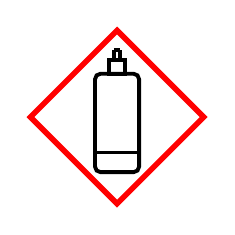
\begin{tikzpicture}
                \draw[draw=red, line width=2pt, fill=white] (0,-1.1) -- (1.1,0) -- (0,1.1) -- (-1.1,0) -- cycle;
                \draw[line width=1.4pt, rounded corners=2pt] (-0.28,-0.7) rectangle (0.28,0.55);
                \draw[line width=1.4pt] (-0.1,0.55) rectangle (0.1,0.72);
                \draw[line width=1.4pt] (-0.04,0.72) -- (-0.04,0.85);
                \draw[line width=1.4pt] (0.04,0.72) -- (0.04,0.85);
                \draw[line width=1.4pt] (-0.04,0.85) -- (0.04,0.85);
                \draw[line width=1pt] (-0.28,-0.45) -- (0.28,-0.45);
            \end{tikzpicture}\\[2pt]
            \textbf{Compressed gas}\\[2pt]
            {\small Gas stored under pressure, may explode when heated. Example: gas cylinders.}
        \end{minipage}
        &
        \begin{minipage}{5.0cm}
            \centering
            
\begin{tikzpicture}
                \draw[draw=red, line width=2pt, fill=white] (0,-1.1) -- (1.1,0) -- (0,1.1) -- (-1.1,0) -- cycle;
                \begin{scope}[rotate=20, shift={(-0.35,0.55)}]
                    \draw[line width=1.2pt] (-0.1,-0.35) -- (-0.1,0.35) arc (180:0:0.1) -- (0.1,-0.35) -- cycle;
                \end{scope}
                \begin{scope}[rotate=-20, shift={(0.35,0.55)}]
                    \draw[line width=1.2pt] (-0.1,-0.35) -- (-0.1,0.35) arc (180:0:0.1) -- (0.1,-0.35) -- cycle;
                \end{scope}
                \draw[line width=1pt] (-0.15,0.15) -- (-0.05,-0.05);
                \draw[line width=1pt] (0.15,0.15) -- (0.05,-0.05);
                \fill[black] (-0.45,-0.15) -- (0.45,-0.15) -- (0.4,-0.3) -- (0.3,-0.18) -- (0.2,-0.32) -- (0.1,-0.16) -- (0,-0.3) -- (-0.1,-0.16) -- (-0.2,-0.3) -- (-0.3,-0.16) -- (-0.4,-0.28) -- cycle;
                \draw[line width=1.2pt] (-0.4,-0.55) .. controls (-0.2,-0.75) and (0.2,-0.75) .. (0.4,-0.55) -- (0.4,-0.85) -- (-0.4,-0.85) -- cycle;
                \draw[line width=0.8pt] (-0.05,-0.6) -- (-0.02,-0.75);
                \draw[line width=0.8pt] (0.1,-0.62) -- (0.13,-0.78);
            \end{tikzpicture}\\[2pt]
            \textbf{Corrosive}\\[2pt]
            {\small Burns skin and eyes, and can destroy metals. Example: bleach, drain cleaner.}
        \end{minipage}
        &
        \begin{minipage}{5.0cm}
            \centering
            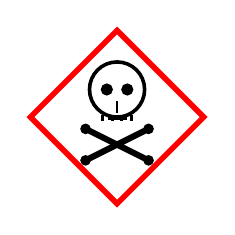
\begin{tikzpicture}
                \draw[draw=red, line width=2pt, fill=white] (0,-1.1) -- (1.1,0) -- (0,1.1) -- (-1.1,0) -- cycle;
                \draw[line width=1.3pt] (0,0.35) circle (0.35);
                \filldraw[black] (-0.13,0.35) circle (0.07);
                \filldraw[black] (0.13,0.35) circle (0.07);
                \draw[line width=1pt] (0,0.2) -- (0,0.05);
                \draw[line width=1pt] (-0.12,-0.02) -- (0.12,-0.02);
                \draw[line width=1pt] (-0.18,-0.05) -- (-0.18,0.02);
                \draw[line width=1pt] (-0.06,-0.05) -- (-0.06,0.02);
                \draw[line width=1pt] (0.06,-0.05) -- (0.06,0.02);
                \draw[line width=1pt] (0.18,-0.05) -- (0.18,0.02);
                \draw[line width=2.2pt] (-0.4,-0.55) -- (0.4,-0.15);
                \draw[line width=2.2pt] (-0.4,-0.15) -- (0.4,-0.55);
                \filldraw[black] (-0.4,-0.55) circle (0.06);
                \filldraw[black] (0.4,-0.15) circle (0.06);
                \filldraw[black] (-0.4,-0.15) circle (0.06);
                \filldraw[black] (0.4,-0.55) circle (0.06);
            \end{tikzpicture}\\[2pt]
            \textbf{Toxic}\\[2pt]
            {\small Can kill or seriously harm you, even in small amounts. Example: some pesticides.}
        \end{minipage}
        \\[9mm]
        \begin{minipage}{5.0cm}
            \centering
            
\begin{tikzpicture}
                \draw[draw=red, line width=2pt, fill=white] (0,-1.1) -- (1.1,0) -- (0,1.1) -- (-1.1,0) -- cycle;
                \draw[line width=5pt, line cap=round] (0,-0.05) -- (0,0.65);
                \filldraw[black] (0,-0.45) circle (0.1);
            \end{tikzpicture}\\[2pt]
            \textbf{Harmful / Irritant}\\[2pt]
            {\small Irritates skin or eyes, or is harmful if swallowed. Example: some detergents.}
        \end{minipage}
        &
        \begin{minipage}{5.0cm}
            \centering
            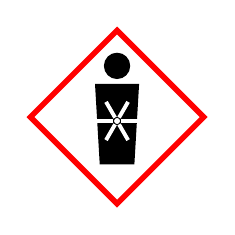
\begin{tikzpicture}
                \draw[draw=red, line width=2pt, fill=white] (0,-1.1) -- (1.1,0) -- (0,1.1) -- (-1.1,0) -- cycle;
                \filldraw[black] (0,0.65) circle (0.16);
                \fill[black] (-0.28,0.42) -- (0.28,0.42) -- (0.22,-0.6) -- (-0.22,-0.6) -- cycle;
                \begin{scope}[shift={(0,-0.05)}]
                    \foreach \a in {0,60,120,180,240,300}{
                        \draw[white, line width=1.4pt] (\a:0.05) -- (\a:0.28);
                    }
                \end{scope}
                \filldraw[white] (0,-0.05) circle (0.03);
            \end{tikzpicture}\\[2pt]
            \textbf{Health hazard}\\[2pt]
            {\small Can cause serious long-term damage (e.g.\ to the lungs). Example: tobacco smoke, asbestos.}
        \end{minipage}
        &
        \begin{minipage}{5.0cm}
            \centering
            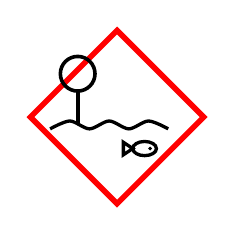
\begin{tikzpicture}
                \draw[draw=red, line width=2pt, fill=white] (0,-1.1) -- (1.1,0) -- (0,1.1) -- (-1.1,0) -- cycle;
                \draw[line width=1.4pt] (-0.5,-0.1) -- (-0.5,0.35);
                \draw[line width=1.3pt] (-0.5,0.55) circle (0.22);
                \draw[line width=1.2pt] plot[smooth] coordinates {(-0.85,-0.15) (-0.6,-0.05) (-0.35,-0.15) (-0.1,-0.05) (0.15,-0.15) (0.4,-0.05) (0.65,-0.15)};
                \draw[line width=1.2pt] (0.35,-0.4) ellipse (0.15 and 0.09);
                \draw[line width=1.2pt] (0.2,-0.4) -- (0.08,-0.32) -- (0.08,-0.48) -- cycle;
                \filldraw[black] (0.42,-0.4) circle (0.015);
            \end{tikzpicture}\\[2pt]
            \textbf{Environmental hazard}\\[2pt]
            {\small Poisonous to plants, fish or other wildlife. Example: some pesticides and solvents.}
        \end{minipage}
    \end{tabular}
    \caption{The nine GHS hazard pictograms: a black symbol on a white background, inside a red diamond.}
\end{figure}

\begin{impt}
    A single product can carry more than one pictogram at the same time (for example, a drain cleaner can be both corrosive and toxic). Always read \textbf{all} the pictograms on a label before using a product.
\end{impt}

\begin{exercise}
    A bottle of concentrated hydrochloric acid shows the \negsubro{corrosive} pictogram, and a bottle of ethanol shows the \negsubro{flammable} pictogram. Explain, in your own words, what danger each pictogram warns about, and say one safety measure you should take with each product.
    \begin{solu}
        The \textbf{corrosive} pictogram warns that the acid can burn the skin and eyes and damage materials on contact, so we should wear gloves and goggles and avoid any contact with skin. \\
        The \textbf{flammable} pictogram warns that ethanol catches fire easily, so we should keep it away from flames and heat sources, such as a lit Bunsen burner.
    \end{solu}
\end{exercise}

\begin{exercise}
    A student is going to heat a test tube containing a liquid with a Bunsen burner and then measure its volume once it has cooled down.
    \begin{enumerate}[label=\letraminuscula]
        \item List the equipment and safety items this student should use for the whole activity.
        \item Explain why the test tube must be pointed away from people while it is being heated.
    \end{enumerate}
    \begin{solu}
        \begin{enumerate}[label=\alph*)]
            \item Safety goggles, lab coat, tongs or a test-tube holder to handle the hot test tube, a Bunsen burner, a test tube, and a graduated cylinder to measure the volume of the liquid once it has cooled.
            \item Heated liquids can splash or the tube's contents can be suddenly expelled (bumping); pointing it away from people prevents anyone from being burnt if this happens.
        \end{enumerate}
    \end{solu}
\end{exercise}

\begin{exercise}
    In a laboratory session, a student eats a sandwich while waiting for an experiment to finish, does not tie back her long hair before lighting the Bunsen burner, and pours the leftover chemical down the sink at the end of the class.
    \begin{enumerate}[label=\letraminuscula]
        \item Identify the three safety violations described.
        \item For each one, explain briefly what should have been done instead.
    \end{enumerate}
    \begin{solu}
        \begin{enumerate}[label=\alph*)]
            \item Eating in the laboratory; working with a flame with loose long hair; disposing of chemical waste down the sink.
            \item Food and drink must never be brought into the laboratory; long hair must always be tied back before using a flame, to avoid it catching fire; chemical waste must be poured into the correct labelled waste container, never down the sink.
        \end{enumerate}
    \end{solu}
\end{exercise}

%----------------------------------------------------------------------------------------

\section*{Summary}

\begin{itemize}
    \item \textbf{Scientific method}: observation, hypothesis, experimentation, analysis of results and conclusions; scientists communicate results using scientific language, based on the SI.
    \item \textbf{Matter}: everything that has mass and occupies space. It forms \textbf{bodies} (defined boundaries) or \textbf{material systems} (no defined boundaries).
    \item \textbf{Properties}: quantitative/qualitative, extensive/intensive, general/characteristic (density, melting and boiling points, solubility, conductivity, hardness).
    \item \textbf{Density and floating}: a substance floats in a liquid if its density is lower than the liquid's, and sinks if it is higher.
    \item \textbf{Isolating a quantity}: do the same operation on both sides of the equation: \(d = m/V\), \(m = d \cdot V\), \(V = m/d\).
    \item \textbf{Quantity, unit, measure}: a quantity is measured by comparing it with a unit; the SI fixes the units, multiples and submultiples for each quantity.
    \item \textbf{Fundamental and derived quantities}: the SI has seven fundamental quantities (length, mass, time, temperature, amount of substance, electric current and luminous intensity); all the others (surface area, volume, density, speed, pressure, energy\ldots) are derived from them.
    \item \textbf{Multiples and submultiples}: prefixes (giga, mega, kilo, hecto, deca, deci, centi, milli, micro, nano) worth a power of 10, used to write measurements with simple numbers.
    \item \textbf{Conversion factor}: a fraction of equal amounts in different units, worth 1, used to change the unit of a quantity without changing its value. The 1 always goes with the bigger unit, and we use powers of 10.
    \item \textbf{Length, mass \& capacity}: steps of \(10\); \textbf{surface area}: square the factor of length (steps of \(10^{2}\)); \textbf{volume}: cube the factor of length (steps of \(10^{3}\)).
    \item \textbf{Volume--capacity}: \(\qty{1}{\cubic\metre} = \qty{1}{\kilo\litre}\); \(\qty{1}{\cubic\dm} = \qty{1}{\litre}\); \(\qty{1}{\cubic\cm} = \qty{1}{\mL}\).
    \item \textbf{Time}: \(\qty{1}{\minute} = \qty{60}{\s}\), \(\qty{1}{\hour} = \qty{3600}{\s}\), \(\qty{1}{\day} = \qty{24}{\hour}\), 1 week = 7 days, 1 year = 365 days. \textbf{Speed} and \textbf{density} need two conversion factors.
    \item \textbf{Scientific notation}: \(a \cdot 10^{n}\), with one non-zero digit before the comma. Big numbers \(\to\) the comma jumps left, positive exponent; small numbers \(\to\) the comma jumps right, negative exponent.
    \item \textbf{Pressure and energy}: \(\qty{1}{\atmospher} = \qty{760}{\mmhg} = \qty{101325}{\Pa}\); \(\qty{1}{\calorie} = \qty{4.18}{\J}\).
    \item \textbf{Instruments}: scales for mass; graduated cylinders, burettes and pipettes for volume (reading at the bottom of the meniscus).
    \item \textbf{Sensitivity, precision and accuracy}: the sensitivity of an instrument is its smallest division; a precise measurement gives many stable decimal places, while an accurate one is close to the real value.
    \item \textbf{Indirect measurement}: a quantity calculated from other, directly measured, quantities (surface area, density, small thicknesses\ldots).
    \item \textbf{Laboratory equipment}: test tubes, beakers, Erlenmeyer flasks, graduated cylinders and Bunsen burners, used together with safety goggles, a lab coat and a fume hood.
    \item \textbf{Safety rules}: always wear protective equipment, never eat or work alone, know where the eyewash station and fire extinguisher are, and dispose of waste correctly.
    \item \textbf{Hazard pictograms (GHS)}: nine standardised symbols, black on white inside a red diamond, that warn about the dangers of a chemical product (explosive, flammable, oxidizing, compressed gas, corrosive, toxic, harmful/irritant, health hazard, environmental hazard).
\end{itemize}

\section{Vocabulary}

\begin{vocabulary}[Scientific method]
    An organised set of steps (observation, hypothesis, experimentation, analysis and conclusions) used to answer questions about nature. \newline
    \textbf{Translation to Spanish}: Método científico
\end{vocabulary}

\begin{vocabulary}[Hypothesis]
    A possible, testable explanation for an observed fact. \newline
    \textbf{Translation to Spanish}: Hipótesis
\end{vocabulary}

\begin{vocabulary}[Matter]
    Everything that occupies space and has mass. \newline
    \textbf{Translation to Spanish}: Materia
\end{vocabulary}

\begin{vocabulary}[Body]
    Matter with defined boundaries. \newline
    \textbf{Translation to Spanish}: Cuerpo
\end{vocabulary}

\begin{vocabulary}[Material system]
    Matter with no defined boundaries. \newline
    \textbf{Translation to Spanish}: Sistema material
\end{vocabulary}

\begin{vocabulary}[Property]
    An aspect of matter that can be evaluated. \newline
    \textbf{Translation to Spanish}: Propiedad
\end{vocabulary}

\begin{vocabulary}[Quantity]
    A property of matter that can be measured. \newline
    \textbf{Translation to Spanish}: Magnitud
\end{vocabulary}

\begin{vocabulary}[Fundamental quantity]
    A quantity defined by itself, without using other quantities (length, mass, time\ldots). \newline
    \textbf{Translation to Spanish}: Magnitud fundamental
\end{vocabulary}

\begin{vocabulary}[Derived quantity]
    A quantity obtained by combining fundamental quantities (surface area, volume, speed\ldots). \newline
    \textbf{Translation to Spanish}: Magnitud derivada
\end{vocabulary}

\begin{vocabulary}[Prefix]
    A word or symbol placed before a unit to form a multiple or a submultiple of it (kilo-, centi-\ldots). \newline
    \textbf{Translation to Spanish}: Prefijo
\end{vocabulary}

\begin{vocabulary}[Multiple / Submultiple]
    A unit bigger / smaller than the base unit by a power of 10. \newline
    \textbf{Translation to Spanish}: Múltiplo / Submúltiplo
\end{vocabulary}

\begin{vocabulary}[Unit]
    A known amount of a quantity used as a reference for measuring. \newline
    \textbf{Translation to Spanish}: Unidad
\end{vocabulary}

\begin{vocabulary}[Density]
    Mass per unit of volume. \newline
    \textbf{Translation to Spanish}: Densidad
\end{vocabulary}

\begin{vocabulary}[Solubility]
    Maximum amount of a solute that can dissolve in \qty{100}{\g} of solvent. \newline
    \textbf{Translation to Spanish}: Solubilidad
\end{vocabulary}

\begin{vocabulary}[Floating]
    Situation in which a substance placed in a liquid stays on the surface because its density is lower than that of the liquid. \newline
    \textbf{Translation to Spanish}: Flotar / Flotación
\end{vocabulary}

\begin{vocabulary}[Sensitivity]
    The smallest amount that an instrument can measure. \newline
    \textbf{Translation to Spanish}: Sensibilidad (apreciación)
\end{vocabulary}

\begin{vocabulary}[Precision]
    How many stable decimal places, or how small a variation, an instrument or measurement can distinguish. \newline
    \textbf{Translation to Spanish}: Precisión
\end{vocabulary}

\begin{vocabulary}[Accuracy]
    How close a measurement is to the real value of the quantity. \newline
    \textbf{Translation to Spanish}: Exactitud
\end{vocabulary}

\begin{vocabulary}[Meniscus]
    Curve formed by the surface of a liquid inside a narrow tube. \newline
    \textbf{Translation to Spanish}: Menisco
\end{vocabulary}

\begin{vocabulary}[Indirect measurement]
    A measurement obtained through calculations from other, direct, measurements. \newline
    \textbf{Translation to Spanish}: Medida indirecta
\end{vocabulary}

\begin{vocabulary}[Conversion factor]
    A fraction of equal amounts expressed in different units, used to change units. \newline
    \textbf{Translation to Spanish}: Factor de conversión
\end{vocabulary}

\begin{vocabulary}[Scientific notation]
    A way of writing a number as a coefficient (from 1 to 9,99\ldots) multiplied by a power of 10. \newline
    \textbf{Translation to Spanish}: Notación científica
\end{vocabulary}

\begin{vocabulary}[Exponent]
    The small number written at the top right of a power; it tells us how many times we multiply (or divide) by 10. \newline
    \textbf{Translation to Spanish}: Exponente
\end{vocabulary}

\begin{vocabulary}[To isolate (a quantity)]
    To leave a quantity alone on one side of an equation, doing the same operation on both sides. \newline
    \textbf{Translation to Spanish}: Despejar (una magnitud)
\end{vocabulary}

\begin{vocabulary}[Hazard pictogram]
    A standardised symbol on a chemical product's label that warns about the type of danger it presents. \newline
    \textbf{Translation to Spanish}: Pictograma de peligrosidad
\end{vocabulary}

\begin{vocabulary}[Corrosive]
    Able to burn the skin and eyes and destroy materials on contact. \newline
    \textbf{Translation to Spanish}: Corrosivo
\end{vocabulary}

\begin{vocabulary}[Flammable]
    Able to catch fire easily. \newline
    \textbf{Translation to Spanish}: Inflamable
\end{vocabulary}

\begin{vocabulary}[Fume hood]
    A ventilated cabinet that extracts dangerous gases or vapours from the laboratory. \newline
    \textbf{Translation to Spanish}: Vitrina de gases / Campana extractora
\end{vocabulary}

\begin{vocabulary}[Safety goggles]
    Glasses that protect the eyes from splashes, dust and vapours. \newline
    \textbf{Translation to Spanish}: Gafas de seguridad
\end{vocabulary}

\begin{vocabulary}[Bunsen burner]
    A gas burner used as a heat source in the laboratory. \newline
    \textbf{Translation to Spanish}: Mechero Bunsen
\end{vocabulary}
